\documentclass[journal, onecolumn, 12pt]{IEEEtran}
\usepackage{cite}
\usepackage[pdftex]{graphicx}
\usepackage{amsmath}
\usepackage{array}

%\usepackage[caption=false,font=footnotesize]{subfig}
\usepackage{stfloats}

\usepackage{url}
\usepackage{color,soul}

\usepackage[utf8]{inputenc}
\usepackage{flushend}
\usepackage{multirow}
\usepackage{multicol}
\usepackage{amssymb}

\usepackage{siunitx}
\usepackage{color}
\usepackage{cite}
\usepackage{colortbl}
\usepackage[table]{xcolor}
\usepackage{booktabs}
\usepackage{datetime}
\usepackage{pdflscape}
\usepackage{hyperref}
\usepackage{url}
\usepackage{pdflscape}
\usepackage{longtable}
\usepackage{float}
\usepackage{tablefootnote}
\usepackage{listings}

%\usepackage{caption}
\usepackage[font=footnotesize]{subcaption}
%\usepackage[left=2.0cm, right=2.0cm, top=2.0cm, bottom=2.0cm]{geometry}

\usepackage[color=green	!20, textsize=scriptsize, textwidth=2.2cm]{todonotes}

\usepackage{tikz}

\hyphenation{op-tical net-works semi-conduc-tor}

% A popular package from the American Mathematical Society that provides
% many useful and powerful commands for dealing with mathematics.
%
% Note that the amsmath package sets \interdisplaylinepenalty to 10000
% thus preventing page breaks from occurring within multiline equations. Use:
\interdisplaylinepenalty=2500
% after loading amsmath to restore such page breaks as IEEEtran.cls normally
% does. amsmath.sty is already installed on most LaTeX systems. The latest
% version and documentation can be obtained at:
% http://www.ctan.org/pkg/amsmath



% declare the path(s) where your graphic files are
\graphicspath{{./figs/}}
% and their extensions so you won't have to specify these with
% every instance of \includegraphics
\DeclareGraphicsExtensions{.pdf,.jpeg,.png}

\definecolor{BlueMunsell}{rgb}{0.0, 0.5, 0.69}


\colorlet{tableheadcolor}{gray!25} % Table header colour = 25% gray
\newcommand{\headcol}{\rowcolor{tableheadcolor}} %
\colorlet{tablerowcolor}{gray!10} % Table row separator colour = 10% gray
\newcommand{\rowcol}{\rowcolor{tablerowcolor}} %
\colorlet{hlrow}{gray!10}
\newcommand{\hlrow}{\rowcolor{hlrow}}
\colorlet{crowcol}{gray!5}
\newcommand{\crowcol}{\rowcolor{crowcol}}
\newcommand{\cellcol}{\cellcolor{white}}
% Command \topline consists of a (slightly modified) \toprule followed by a \heavyrule rule of colour tableheadcolor (hence, 2 separate rules)
\newcommand{\topline}{\arrayrulecolor{black}\specialrule{0.1em}{\abovetopsep}{0pt}%
    \arrayrulecolor{tableheadcolor}\specialrule{\belowrulesep}{0pt}{0pt}%
    \arrayrulecolor{black}}

% Command \midline consists of 3 rules (top colour tableheadcolor, middle colour black, bottom colour white)
\newcommand{\midline}{\arrayrulecolor{tableheadcolor}\specialrule{\aboverulesep}{0pt}{0pt}%
    \arrayrulecolor{black}\specialrule{\lightrulewidth}{0pt}{0pt}%
    \arrayrulecolor{white}\specialrule{\belowrulesep}{0pt}{0pt}%
    \arrayrulecolor{black}\hline}

% Command \rowmidlinecw consists of 3 rules (top colour tablerowcolor, middle colour black, bottom colour white)
\newcommand{\rowmidlinecw}{\arrayrulecolor{tablerowcolor}\specialrule{\aboverulesep}{0pt}{0pt}%
    \arrayrulecolor{black}\specialrule{\lightrulewidth}{0pt}{0pt}%
    \arrayrulecolor{white}\specialrule{\belowrulesep}{0pt}{0pt}%
    \arrayrulecolor{black}}

% Command \rowmidlinewc consists of 3 rules (top colour white, middle colour black, bottom colour tablerowcolor)
\newcommand{\rowmidlinewc}{\arrayrulecolor{white}\specialrule{\aboverulesep}{0pt}{0pt}%
    \arrayrulecolor{black}\specialrule{\lightrulewidth}{0pt}{0pt}%
    \arrayrulecolor{tablerowcolor}\specialrule{\belowrulesep}{0pt}{0pt}%
    \arrayrulecolor{black}}

% Command \rowmidlinew consists of 1 white rule
\newcommand{\rowmidlinew}{\arrayrulecolor{white}\specialrule{\aboverulesep}{0pt}{0pt}%
    \arrayrulecolor{black}}

% Command \rowmidlinec consists of 1 tablerowcolor rule
\newcommand{\rowmidlinec}{\arrayrulecolor{tablerowcolor}\specialrule{\aboverulesep}{0pt}{0pt}%
    \arrayrulecolor{black}}

% Command \bottomline consists of 2 rules (top colour
\newcommand{\bottomline}{\arrayrulecolor{white}\specialrule{\aboverulesep}{0pt}{0pt}%
    \arrayrulecolor{black}\specialrule{\heavyrulewidth}{0pt}{\belowbottomsep}}%
\newcommand{\bottomlinec}{\arrayrulecolor{tablerowcolor}\specialrule{\aboverulesep}{0pt}{0pt}%
    \arrayrulecolor{black}\specialrule{\heavyrulewidth}{0pt}{\belowbottomsep}}%
\newcommand{\bottomlinehc}{\arrayrulecolor{tableheadcolor}\specialrule{\aboverulesep}{0pt}{0pt}%
    \arrayrulecolor{black}\specialrule{\heavyrulewidth}{0pt}{\belowbottomsep}}%

%\newcommand{\etal}[1]{#1~\textit{et~al.}}
\newcommand{\etal}[1]{#1~et~al.}
\newcommand{\TODO}[1]{\textcolor{blue}{\textbf{TODO:} \textbf{#1}}}

\setlength{\heavyrulewidth}{0.1em}
\newcommand {\otoprule}{\midrule[\heavyrulewidth]}
\renewcommand{\arraystretch}{1.1}

\providecommand{\redmark}[1]{{\protect\color{red}{#1}}}
\providecommand{\bluemark}[1]{{\protect\color{blue}{#1}}}

\let\mcol\multicolumn
\let\ml\multirow

\renewcommand{\vec}[1]{\mathbf{#1}}

\newcommand{\todox}[2][1=]{\todo[size=\tiny,#1]{#2}}
\newcommand{\unsure}[2][1=]{\todo[linecolor=red,backgroundcolor=red!25,bordercolor=red,size=\tiny,#1]{#2}}
\newcommand{\change}[2][1=]{\todo[linecolor=blue,backgroundcolor=blue!25,bordercolor=blue,size=\tiny,#1]{#2}}

\newcommand{\review}[1]{\textcolor{red}{#1}}


% Definitions of handy macros can go here

\newcommand{\dataset}{{\cal D}}
\newcommand{\fracpartial}[2]{\frac{\partial #1}{\partial  #2}}
\newcommand{\expnumber}[2]{{#1}\times10^{#2}}
\newcommand{\highlight}[1]{\tikz[baseline]{\node[rounded corners,fill=green!25, anchor=base]{$\mathbf{#1}$}}}



 
\definecolor{codegreen}{rgb}{0,0.6,0}
\definecolor{codegray}{rgb}{0.5,0.5,0.5}
\definecolor{codepurple}{rgb}{0.58,0,0.82}
\definecolor{backcolour}{rgb}{0.95,0.95,0.92}

\lstdefinestyle{fancyterminal}{
    backgroundcolor=\color{backcolour},   
    commentstyle=\color{codegreen},
    keywordstyle=\color{magenta},
    numberstyle=\tiny\color{codegray},
    stringstyle=\color{codepurple},
    basicstyle=\scriptsize\ttfamily,
    breakatwhitespace=false,         
    breaklines=true,                 
    captionpos=b,                    
    keepspaces=true,
%    numbers=left,                    
    numbersep=5pt,                  
    showspaces=false,                
    showstringspaces=false,
    showtabs=false,                  
    tabsize=2
}

\lstdefinestyle{terminal}
{
    backgroundcolor=\color{black},
    basicstyle=\scriptsize\color{white}\ttfamily
    commentstyle=\color{codegreen},
    keywordstyle=\color{magenta},
    numberstyle=\tiny\color{codegray},
    stringstyle=\color{codepurple},
    breakatwhitespace=false,         
    breaklines=true,                 
    captionpos=b,                    
    keepspaces=true,
%    numbers=left,                    
    numbersep=5pt,                  
    showspaces=false,                
    showstringspaces=false,
    showtabs=false,                  
    tabsize=2
}

%\lstset{style=mystyle}


% Set the space between lines
\linespread{1.5}

\begin{document}
    %
    % paper title
    % Titles are generally capitalized except for words such as a, an, and, as,
    % at, but, by, for, in, nor, of, on, or, the, to and up, which are usually
    % not capitalized unless they are the first or last word of the title.
    % Linebreaks \\ can be used within to get better formatting as desired.
    % Do not put math or special symbols in the title.
    \title{Technical Report (Deliverable E4)}
    %
    %
    % author names and IEEE memberships
    % note positions of commas and nonbreaking spaces ( ~ ) LaTeX will not break
    % a structure at a ~ so this keeps an author's name from being broken across
    % two lines.
    % use \thanks{} to gain access to the first footnote area
    % a separate \thanks must be used for each paragraph as LaTeX2e's \thanks
    % was not built to handle multiple paragraphs
    %
    
    \author{
        Ricardo da S. Torres,
        Allan~Pinto,
        Manuel C\'{o}rdova Neira,\\
        Jose Luis Flores Campana,
        Luis G. L. Decker, \\
        Andreza Santos, and
        Jhonatas S. Concei\c{c}\~{a}o

        \thanks{All authors are with the Institute of Computing, University of Campinas (Unicamp), Av. Albert Einstein, 1251, Campinas, SP, Brazil, 13083-852. E-mail: rtorres@ic.unicamp.br.}% <-this % stops a space

%        \thanks{Manuscript received ...; revised ....}
        }
    
    % note the % following the last \IEEEmembership and also \thanks - 
    % these prevent an unwanted space from occurring between the last author name
    % and the end of the author line. i.e., if you had this:
    % 
    % \author{....lastname \thanks{...} \thanks{...} }
    %                     ^------------^------------^----Do not want these spaces!
    %
    % a space would be appended to the last name and could cause every name on that
    % line to be shifted left slightly. This is one of those "LaTeX things". For
    % instance, "\textbf{A} \textbf{B}" will typeset as "A B" not "AB". To get
    % "AB" then you have to do: "\textbf{A}\textbf{B}"
    % \thanks is no different in this regard, so shield the last } of each \thanks
    % that ends a line with a % and do not let a space in before the next \thanks.
    % Spaces after \IEEEmembership other than the last one are OK (and needed) as
    % you are supposed to have spaces between the names. For what it is worth,
    % this is a minor point as most people would not even notice if the said evil
    % space somehow managed to creep in.
    
    
    
    % The paper headers
%    \markboth{IEEE XXX,~Vol.~XX, No.~X, August~XXXX}
%    {Shell \MakeLowercase{\textit{et al.}}: Bare Demo of IEEEtran.cls for IEEE Journals}

    % The only time the second header will appear is for the odd numbered pages
    % after the title page when using the twoside option.
    % 
    % *** Note that you probably will NOT want to include the author's ***
    % *** name in the headers of peer review papers.                   ***
    % You can use \ifCLASSOPTIONpeerreview for conditional compilation here if
    % you desire.
    
    
    
    
    % If you want to put a publisher's ID mark on the page you can do it like
    % this:
    %\IEEEpubid{0000--0000/00\$00.00~\copyright~2015 IEEE}
    % Remember, if you use this you must call \IEEEpubidadjcol in the second
    % column for its text to clear the IEEEpubid mark.
        
    % use for special paper notices
    %\IEEEspecialpapernotice{(Invited Paper)}
    
    % make the title area
    \maketitle
    
    % Entregável 4 (E4) em 12/2018: primeiro protótipo relacionado à implementação de técnicas de reconhecimento de texto. Este protótipo contemplará soluções encontradas em bibliotecas públicas, validadas no contexto de dispositivos com restrição de processamento.

\begin{abstract}

In this technical report, we present a prototype that encompasses traditional and recent methods proposed for text spotting and recognition problems, considering both non-deep and deep-learning-based approaches. We also present architectural and functional overviews of the prototype, as well as describe deployment procedures and possible usage scenarios. This report is related to the ongoing project named Multi-Lingual Text Spotting and Recognition (MLTSR), which is being developed in the context of the collaboration between Samsung R\&D Institute Brazil (SRBR) and University of Campinas (Unicamp), and it refers to the fourth deliverable (E4) planned for this project.

\end{abstract}

% Note that keywords are not normally used for peerreview papers.
\begin{IEEEkeywords}
    Text Spotting, Text Recognition, End-to-end Solutions, Scene Text Detection, Feature Engineering, Supervised Feature Learning, Convolutional Neural Networks, Recurrent Neural Network, Deep Learning, Prototype
\end{IEEEkeywords}

    \section{Introduction}
\label{sec:introduction}
% Entregável 4 (E4) em 12/2018: primeiro protótipo relacionado à implementação de técnicas de reconhecimento de texto. Este protótipo contemplará soluções encontradas em bibliotecas públicas, validadas no contexto de dispositivos com restrição de processamento.

This technical report is related to the ongoing project named Multi-Lingual Text Spotting and Recognition (MLTSR), which is being developed in the context of the collaboration between Samsung R\&D Institute Brazil (SRBR) and University of Campinas (Unicamp). This document refers to the fourth deliverable (E4) planned for this project. Deliverable E4 concerns with the development of a prototype, which encompasses end-to-end text recognition methods. In this document, we present an overview of the developed prototype, as well as instructions of how to use it in order to reproduce the results reported in deliverable E3.

The developed docker-based prototype is composed of three modules: \textit{text spotting}, \textit{post-processing}, and \textit{text recognition} modules. Fig.~\ref{fig:prototype-overview-simple} provides a conceptual overview of the prototype and its components. The text spotting applications refer to methods used for detecting candidate regions in a scene, while the post-processing methods are used to refine detection results. The module dedicated to text recognition applications includes a set of methods that focus on the recognition of texts, given a detected text region image. We provide a command-line interface that enables the creation of all docker images utilized in this prototype, as well as supports the execution of combinations of the components provided in the three modules. In such a way, text spotting and end-to-end recognition applications may be created and executed independently, depending on the users' needs.
%
\begin{figure}
    \centering
    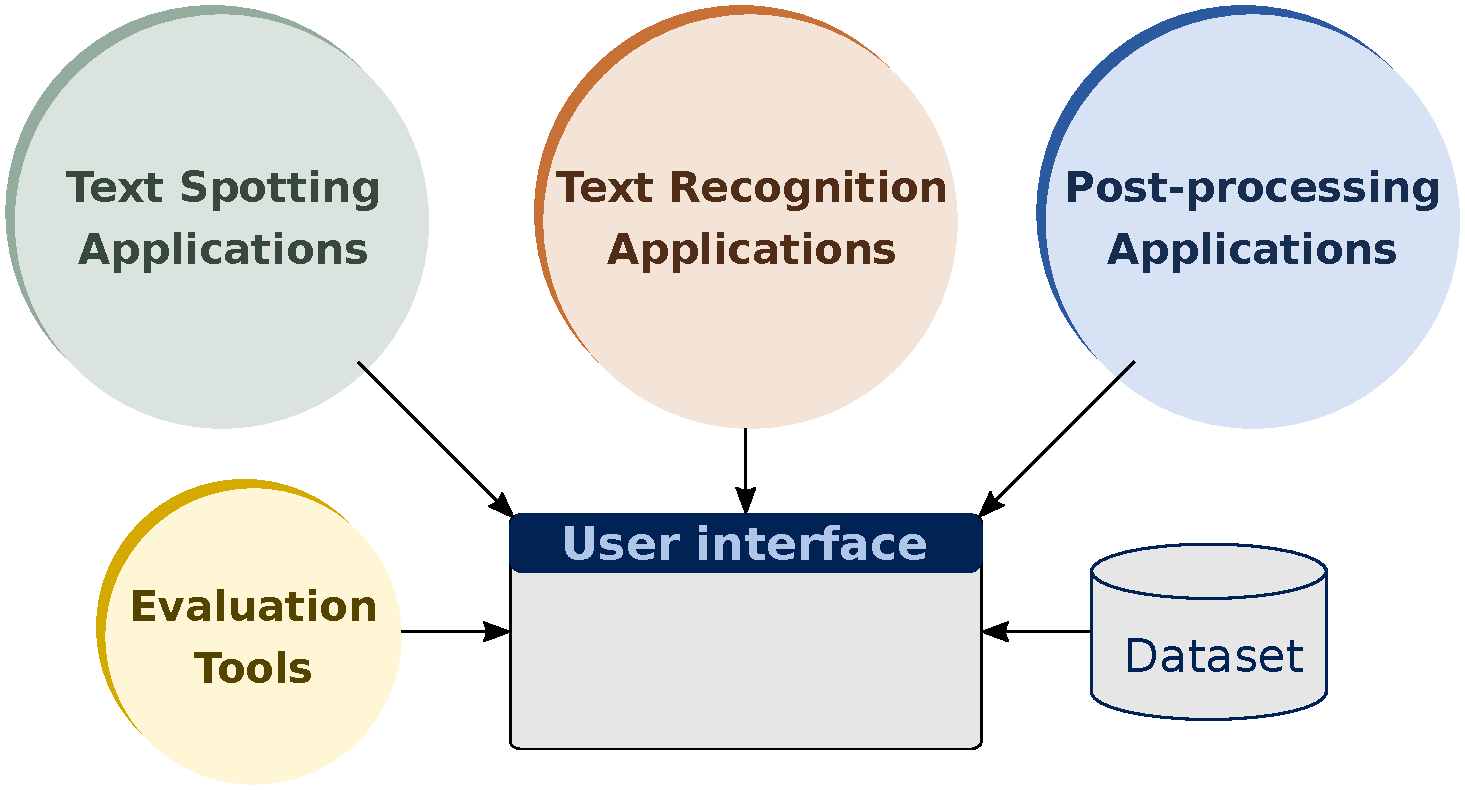
\includegraphics[width=0.6\textwidth]{figs/prototype-overview-simple.pdf}
    \caption{Overview of the main components of the prototype. The text spotting applications refer to methods used for detecting candidate regions in a scene, while the post-processing applications are used to refine detection results. The text recognition applications provide the components responsible for recognizing texts found within detected regions.}
    \label{fig:prototype-overview-simple}
\end{figure}

We organized the remainder of this document as follows: Section~\ref{sec:overview} provides an overview of the prototype; Section~\ref{sec:usage-scenario} presents a comprehensive usage scenario of the prototype, concerning the execution of different end-to-end recognition methods; finally, Section~\ref{sec:conclusions} presents our final remarks and directions for future investigations.
    
\section{The Prototype}
\label{sec:overview}

This section presents the developed prototype, discussing its architecture (Section~\ref{sec:architecture}), implementation issues (Section~\ref{sec:implementation}), deployment procedures (Section~\ref{sec:instalation}), and usage examples (Section~\ref{sec:using}).

\subsection{Architectural Overview}
\label{sec:architecture}

Fig.~\ref{fig:prototype-overview-simple} provides a conceptual overview of the prototype and its main components.
The text recognition applications provide the components responsible for recognizing the text found within detected regions. The text spotting module includes container applications that encapsulate the text spotting methods related to deliverables E2 and E3. The post-processing module comprises two containers: the post-processing method developed by the Samsung Research (SRBR) team, and an improved version developed at Unicamp. Similarly, the text recognition module provides three containers that encapsulate the three recognition methods presented in deliverable E3: Tesseract, Long Short-Term Memory (LSTM), and Convolutional Recurrence Neural Network (CRNN) recognition methods.

Table~\ref{tab:methods-available} summarizes the text detection and recognition methods handled in the prototype. As we can observe, we consider non-deep and deep-learning-based solutions.\footnote{Readers may refer to Deliverables E1 and E3 to find descriptions of such methods.}
%
\begin{table}[H]
    \centering
    \caption{Method for text detection and recognition available in the prototype.}
    \label{tab:methods-available}
    \begin{tabular}{ll|p{5.5cm}}
        \hline
        \topline
        \headcol
        \textbf{Type}   & \textbf{Methods for Text Detection}       & \textbf{Methods for Text Recognition} \\ \midline
        & - SnooperText                             	& - Tesseract v.3                         \\
        & - Canny Text Detection                    & - Tesseract with Post-processing provided \\
        & - MSER-SWT Text Detection                 &   by Samsung Team   \\
        & - Multi-Lingual Text Detection            & - Tesseract with Improved Post-processing \\
        & - FASText                                 &                                       \\
        
        \ml{-6}{*}{Non-Deep Methods}
        & - Scene Text Recognition (pretrained models) &                                       \\ \hline \hline
        & - SSTD                                       & - LSTM (Tesseract v.4)                  \\
        & - TextBoxes                                  & - CRNN                                  \\
        & - TextBoxes++                                &                                       \\
        & - SSD-MobilenetV2                            &                                       \\
        & - YOLOv3                                     &                                       \\
        
        \ml{-6}{*}{Deep Learning-Based 
            Methods}        & - SqueezeDet                                 &                                       \\
        \bottomlinec
    \end{tabular}
\end{table}
\footnotesize{$^{\star}$Some components are not fully integrated to the prototype as a docker application. We will provide a Dockerfile for all these components soon.}


\subsection{Implementation Overview}
\label{sec:implementation}


The prototype developed in this deliverable contains several applications with different software dependencies, including libraries, programming tools, and the base operating system. The integration of all these pieces of software into a single prototype is very challenging and we opted to package all applications that compose the prototype using the Docker\footnote{\url{https://www.docker.com/} (As of Dec. 2018).} technology. Docker is an open source platform (Apache License 2.0) for operating-system-level virtualization. Docker provides a standardized unit software for packaging the source code and all its dependencies, including system tools, system libraries, and settings.

In this prototype, we implement \textit{Dockerfiles} that automatically package the source code, install its dependencies, install and compile source codes, and finally builds a docker image able to run the application as a command line, in a proper software platform. Fig.~\ref{fig:overview-prototype} illustrates an overview of the architecture of the prototype. We built two base docker images, which contain some common libraries required for running non-deep- and deep-learning-based methods. These base docker images are used to build the docker images for the applications.
%
\begin{figure}
    \centering
    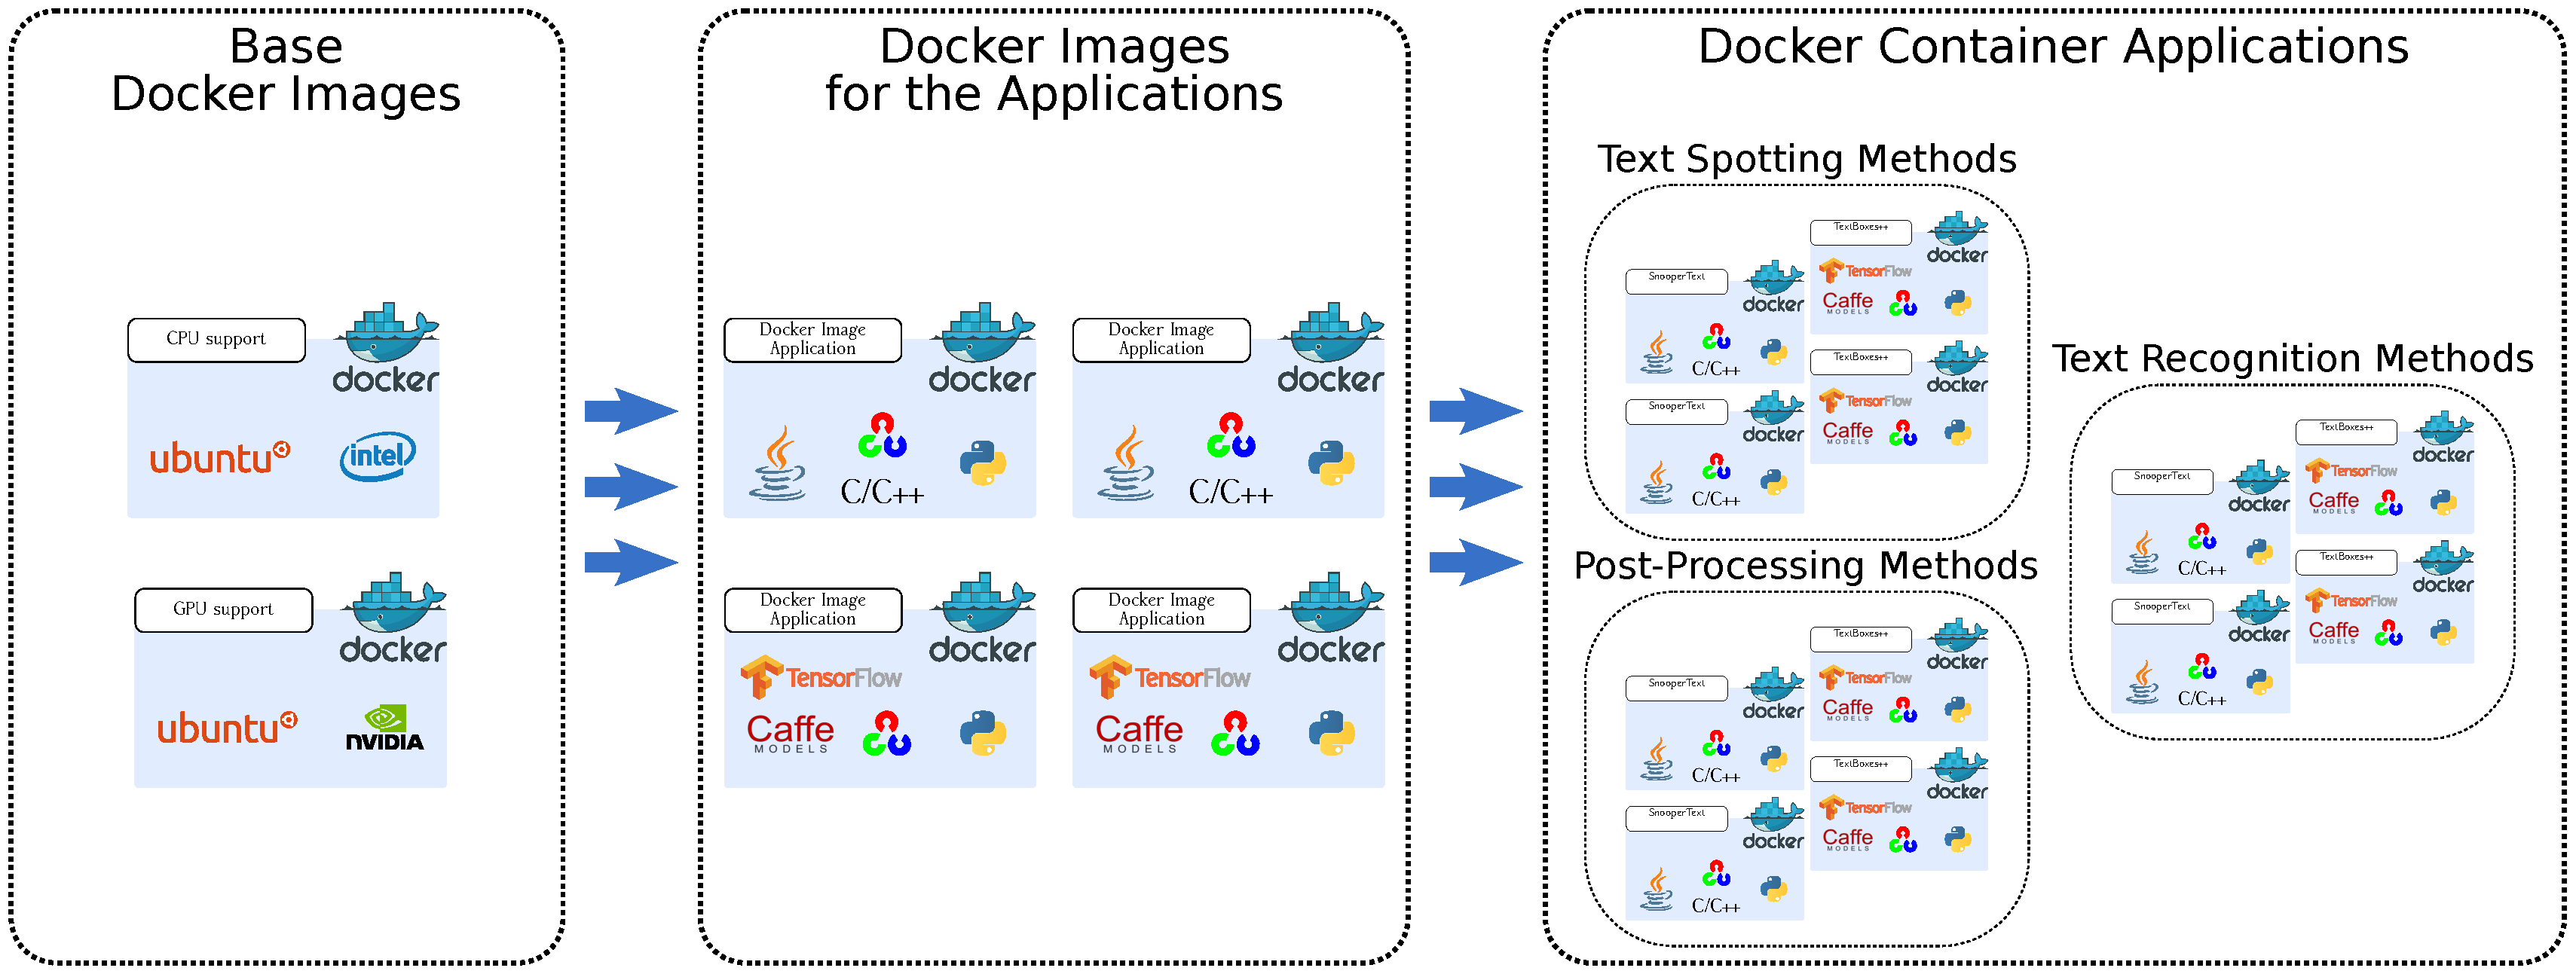
\includegraphics[width=0.98\textwidth]{figs/prototype-overview.pdf}
    \caption{Architectural overview of the prototype.}
    \label{fig:overview-prototype}
\end{figure}


\subsection{Deploying the Prototype}
\label{sec:instalation}

This section presents the procedures for deploying the prototype.

\subsubsection{How to Build the Docker Base Images}
\label{sec:build-docker-base-images}

We provide Dockerfiles for all docker containers used in this prototype. Specially, we built two Dockerfiles, which are used as base for all components of the prototype. With this, we reduce the time to generate the docker containers and we standardize some common software, tools and libraries (e.g., OpenCV, CUDA, OpenBLAS).

Suppose that the environment variable \textsc{ROOT\_DIR} points to the path where the prototype was downloaded. To build the docker base images, the following commands can be used:
%
\begin{lstlisting}[style=fancyterminal]
 $ cd $ROOT_DIR
 $ ./0-main-build-docker-base-images.sh
\end{lstlisting}

This shell script calls the scripts responsible for building the docker base images, whose Dockerfiles are located in \textsc{\$ROOT\_DIR/misc/base-dockerfiles} directory. To see if the base images were built correctly, the command \emph{\$ docker images} may be used. As result of its use, two docker images, named as \textit{unicamp-mltsr-deliverable-e4/base-cpu-support:4.0} and \textit{unicamp-mltsr-deliverable-e4/base-gpu-support:4.0}, are identified (see listing below).

\begin{lstlisting}[style=fancyterminal]
 REPOSITORY                                        TAG                     IMAGE ID    
 unicamp-mltsr-deliverable-e4/base-cpu-support     4.0                     d822492254bf
 unicamp-mltsr-deliverable-e4/base-gpu-support     4.0                     d9cad4ce0273
 ubuntu                                            16.04                   b0ef3016420a
 nvidia/cuda                                       8.0-devel-ubuntu16.04   d610c8c58845
\end{lstlisting}



\subsubsection{How to Build the Docker Image Applications}
\label{sec:build-docker-image-app}

The Docker Image Applications form the most important component in our prototype, since they contain the implementation source code (and its compiled version) of text detection and recognition methods. Those applications contain the \textsc{ENTRYPOINT} of their respective docker container. The \textsc{ENTRYPOINT} is a Dockerfile instruction used to set the image's main command in such a way that a docker container can be run by means of a command line in a Linux terminal. The Dockerfiles also contain the instruction needed to install the software requirements of the applications and also instructions to automatically compile the source code. Therefore, there is no need for the direct use of docker containers to compile libraries and source codes manually.

To build the docker images needed to run the applications, the following command in the terminal can be used:
%
\begin{lstlisting}[style=fancyterminal]
 $ ./0-main-build-docker-images-text-spotting.sh
 $ ./0-main-build-docker-images-text-recognition.sh
 $ ./0-main-build-docker-images-post-processing.sh
 $ ./0-main-build-docker-images-evaluations.sh
\end{lstlisting}

These shell scripts call the scripts responsible for building the docker images that contain the text spotting, post-processing, text recognition methods, as well as the docker containers used to evaluate the text spotting and text recognition methods. To see if the docker images were built correctly, the command \emph{\$ docker images} may be used to have access to information regarding the built docker images. We provided a demo script (\textit{demo-00-testing-build-docker-images.sh}) that builds all docker images required to use this prototype.

\subsection{Using the Prototype}
\label{sec:using}

\subsubsection{Running a Text Spotting Application}

We provide shell scripts to run a text spotting application by choosing the method to be used to detect the candidate regions and also to run all text spotting methods available in this prototype. The option to run post-processing methods on top of text spotting method's output is also available.  

To run all text spotting methods available, the following command can be used:

\begin{lstlisting}[style=fancyterminal]
 $ ./1-main-text-spotting-methods.sh \
        --dataset_path /path/to/datasets \
        --working_path /path/to/working/directory/ \
        --dataset_id icdarXX \
        --text_spotting_method_id all-methods
\end{lstlisting}

To see all options available, the following command can be used:
\begin{lstlisting}[style=fancyterminal]
 $ ./1-main-text-spotting-methods.sh --help
 Usage: ./1-main-text-spotting-methods.sh [options]
 
 options:
 -h, --help                show brief help
 --dataset_path            path to dataset directory
 --working_path            path to output directory
 --dataset_id              dataset identifier (choose from icdar11, icdar13, icdar15)
 --text_spotting_method_id text spotting method identifier (choose from options below)
       options:
           all-methods (default)
           deliverable-e2-canny
           deliverable-e2-snoopertext
           deliverable-e4-canny
           deliverable-e4-snoopertext
           deliverable-e4-mserswt
           deliverable-e4-multiligual
           deliverable-e4-scenetext
           deliverable-e4-ssd-mobilenetv2
           deliverable-e4-sstd
           deliverable-e4-squeezedet
           deliverable-e4-yolov3
\end{lstlisting}

To run the post-processing methods available on top of all text spotting methods, the following command can be used:

\begin{lstlisting}[style=fancyterminal]
 $ ./2-main-postprocessing.sh  
        --dataset_path /path/to/datasets \
        --working_path /path/to/working/directory/ \
        --dataset_id icdarXX \
        --text_spotting_method_id all-methods \
        --postprocessing_method_id all-methods
\end{lstlisting}

To see all options available, the following command can be used:
\begin{lstlisting}[style=fancyterminal]
 $ ./2-main-postprocessing.sh --help
 Usage: ./2-main-postprocessing.sh [options]
 
 options:
 -h, --help                show brief help
 --dataset_path            path to dataset directory
 --working_path            path to output directory
 --dataset_id              dataset identifier (choose from icdar11, icdar13, icdar15)
 --text_spotting_method_id text spotting method identifier (choose from options below)
       options:
           all-methods (default)
           deliverable-e2-canny
           deliverable-e2-snoopertext
           deliverable-e4-canny
           deliverable-e4-snoopertext
           deliverable-e4-mserswt
           deliverable-e4-multiligual
           deliverable-e4-scenetext
           deliverable-e4-ssd-mobilenetv2
           deliverable-e4-sstd
           deliverable-e4-squeezedet
           deliverable-e4-yolov3
 --postprocessing_method_id post-processing method identifier (choose from options below)
       options:
           all-methods (default)
           postprocessing-samsung
           postprocessing-improved
\end{lstlisting}

Finally, to evaluate the localizations obtained with text spotting methods, as well as the improvements obtained with the post-processing methods, the following command can be used:
\begin{lstlisting}[style=fancyterminal]
 $ ./4-main-spotting-evaluation.sh 
        --dataset_path /path/to/datasets \
        --working_path /path/to/working/directory/ \
        --dataset_id icdarXX \
        --text_spotting_method_id all-methods \
        --postprocessing_method_id all-methods
\end{lstlisting}

To see all options available, the following command can be used:
\begin{lstlisting}[style=fancyterminal]
 $ ./4-main-spotting-evaluation.sh --help
 Usage: ./4-main-spotting-evaluation.sh [options]
 
 options:
 -h, --help                show brief help
 --dataset_path            path to dataset directory
 --working_path            path to output directory
 --dataset_id              dataset identifier (choose from icdar11, icdar13, icdar15)
 --text_spotting_method_id text spotting method identifier (choose from options below)
       options:
           all-methods (default)
           deliverable-e2-canny
           deliverable-e2-snoopertext
           deliverable-e4-canny
           deliverable-e4-snoopertext
           deliverable-e4-mserswt
           deliverable-e4-multiligual
           deliverable-e4-scenetext
           deliverable-e4-ssd-mobilenetv2
           deliverable-e4-sstd
           deliverable-e4-squeezedet
           deliverable-e4-yolov3
 --postprocessing_method_id post-processing method identifier (choose from options below)
       options:
           all-methods (default)
           none
           postprocessing-improved
           postprocessing-samsung
\end{lstlisting}



\subsubsection{Running an End-to-End Recognition Application}

We also provide a shell script to run an end-to-end solution by choosing the text spotting methods used to detect the candidate regions, the post-processing method to improve the text detection rates, and the text recognition methods used to determine the texts found within detected candidate regions.

Assume that the execution of a text spotting application was performed as described in the previous section. To run the text recognition methods, available in this prototype, on top of the text spotting results, the following command can be used:

\begin{lstlisting}[style=fancyterminal]
 $ ./3-main-recognition.sh \
        --dataset_path /path/to/datasets \
        --working_path /path/to/working/directory/ \
        --dataset_id icdarXX \
        --text_spotting_method_id all-methods \
        --postprocessing_method_id all-methods \
        --text_recognition_method_id all-methods
\end{lstlisting}

To see all options available, the following command can be used:

\begin{lstlisting}[style=fancyterminal]
 $ ./3-main-recognition.sh --help
 Usage: ./3-main-recognition.sh [options]
 
 options:
 -h, --help                show brief help
 --dataset_path            path to dataset directory
 --working_path            path to output directory
 --dataset_id              dataset identifier (choose from icdar11, icdar13, icdar15)
 --text_spotting_method_id text spotting method identifier (choose from options below)
       options:
           all-methods (default)
           deliverable-e2-canny
           deliverable-e2-snoopertext
           deliverable-e4-canny
           deliverable-e4-snoopertext
           deliverable-e4-mserswt
           deliverable-e4-multiligual
           deliverable-e4-scenetext
           deliverable-e4-ssd-mobilenetv2
           deliverable-e4-sstd
           deliverable-e4-squeezedet
           deliverable-e4-yolov3
 --postprocessing_method_id post-processing method identifier (choose from options below)
       options:
           all-methods (default)
           none
           postprocessing-improved
           postprocessing-samsung
 --text_recognition_method_id recognition method identifier (choose from options below)
       options:
           all-methods (default)
           deliverable-e4-tesseract
           deliverable-e4-lstm
           deliverable-e4-crnn
\end{lstlisting}


Finally, to evaluate the recognition methods executed on top of all text recognition methods, as well as the improvements obtained with the post-processing methods, the following command can be used:
\begin{lstlisting}[style=fancyterminal]
 $ ./4-main-recognition-evaluation.sh 
        --dataset_path /path/to/datasets \
        --working_path /path/to/working/directory/ \
        --dataset_id icdarXX \
        --text_spotting_method_id all-methods \
        --postprocessing_method_id all-methods \
        --text_recognition_method_id all-methods
\end{lstlisting}

To see all options available, the following command can be used:
\begin{lstlisting}[style=fancyterminal]
 $ ./4-main-recognition-evaluation.sh --help
 Usage: ./4-main-recognition-evaluation.sh [options]
 
 options:
 -h, --help                show brief help
 --dataset_path            path to dataset directory
 --working_path            path to output directory
 --dataset_id              dataset identifier (choose from icdar11, icdar13, icdar15)
 --text_spotting_method_id text spotting method identifier (choose from options below)
       options:
           all-methods (default)
           deliverable-e2-canny
           deliverable-e2-snoopertext
           deliverable-e4-canny
           deliverable-e4-snoopertext
           deliverable-e4-mserswt
           deliverable-e4-multiligual
           deliverable-e4-scenetext
           deliverable-e4-ssd-mobilenetv2
           deliverable-e4-sstd
           deliverable-e4-squeezedet
           deliverable-e4-yolov3
 --postprocessing_method_id post-processing method identifier (choose from options below)
       options:
           all-methods (default)
           none
           postprocessing-improved
           postprocessing-samsung
 --text_recognition_method_id recognition method identifier (choose from options below)
       options:
           all-methods (default)
           deliverable-e4-tesseract
           deliverable-e4-lstm
           deliverable-e4-crnn

\end{lstlisting}


\section{Usage Scenarios}
\label{sec:usage-scenario}

In this section, we provide an overview of a possible usage of the prototype considering scenarios, in which a user wants to reproduce the results of a text spotting and text recognition solution, both with and without the use of post-processing methods. We also provide these and other demos along with prototype. Hereinafter, we are assuming that all images were built as described in Sections~\ref{sec:build-docker-base-images}~and~\ref{sec:build-docker-image-app}, and that dataset to be used is located in {\footnotesize \ttfamily /dataset/ICDAR11/TEXT\_LOCALIZATION/TEST/Challenge1\_Test\_Task12\_Images}.

\subsection{Running the Snooper Text Detection combined with Tesseract recognition method.}

To run the Snooper Text Detection, the following command can be used:
\begin{lstlisting}[style=fancyterminal]
 $ ./1-main-text-spotting-methods.sh \
    --dataset_path /dataset/ICDAR11/TEXT_LOCALIZATION/TEST/Challenge1_Test_Task12_Images \
    --working_path /working \
    --dataset_id icdar11 \
    --text_spotting_method_id deliverable-e2-snoopertext

\end{lstlisting}

To run the Improved post-processing provided by the Unicamp Team, the following command can be used:

\begin{lstlisting}[style=fancyterminal]
 $ ./2-main-postprocessing.sh \
    --dataset_path /dataset/ICDAR11/TEXT_LOCALIZATION/TEST/Challenge1_Test_Task12_Images \
    --working_path /working \
    --dataset_id icdar11 \
    --text_spotting_method_id deliverable-e2-snoopertext \
    --postprocessing_method_id postprocessing-improved
\end{lstlisting}

To run the Tesseract recognizer on top of the raw localizations detected by the Snooper Text Detection, the following command can be used:
\begin{lstlisting}[style=fancyterminal]
 $ ./3-main-recognition.sh \
    --dataset_path /dataset/ICDAR11/TEXT_LOCALIZATION/TEST/Challenge1_Test_Task12_Images \
    --working_path /working \
    --dataset_id icdar11 \
    --text_spotting_method_id deliverable-e2-snoopertext \
    --postprocessing_method_id none \
    --text_recognition_method_id deliverable-e4-tesseract
\end{lstlisting}

To evaluate the performance results for the text spotting task without post-processing, the following command can be used:
\begin{lstlisting}[style=fancyterminal]
 $ ./4-main-spotting-evaluation.sh \
    --dataset_path /dataset/ICDAR11/TEXT_LOCALIZATION/TEST/Challenge1_Test_Task12_Images \
    --working_path /working \
    --dataset_id icdar11 \
    --text_spotting_method_id deliverable-e4-snoopertext \
    --postprocessing_method_id none
\end{lstlisting}

To evaluate the performance results for the text spotting task with post-processing, the following command can be used:
\begin{lstlisting}[style=fancyterminal]
 $ ./4-main-spotting-evaluation.sh \
    --dataset_path /dataset/ICDAR11/TEXT_LOCALIZATION/TEST/Challenge1_Test_Task12_Images \
    --working_path /working \
    --dataset_id icdar11 \
    --text_spotting_method_id deliverable-e2-snoopertext \
    --postprocessing_method_id postprocessing-improved
\end{lstlisting}

Finally, to evaluate the performance results for the text recognition task with post-processing, the following command can be used:
\begin{lstlisting}[style=fancyterminal]
 $ ./4-main-recognition-evaluation.sh \
    --dataset_path /dataset/ICDAR11/TEXT_LOCALIZATION/TEST/Challenge1_Test_Task12_Images \
    --working_path /working \
    --dataset_id icdar11 \
    --text_spotting_method_id deliverable-e2-snoopertext \
    --postprocessing_method_id postprocessing-improved \
    --text_recognition_method_id deliverable-e4-tesseract
\end{lstlisting}

\subsection{Running the Scene Text Recognition combined with Tesseract recognition method.}

To run the Scene Text Detection, please use the following command:
\begin{lstlisting}[style=fancyterminal]
 $ ./1-main-text-spotting-methods.sh \
    --dataset_path /dataset/ICDAR11/TEXT_LOCALIZATION/TEST/Challenge1_Test_Task12_Images \
    --working_path/working \
    --dataset_id icdar11 \
    --text_spotting_method_id deliverable-e4-scenetext
\end{lstlisting}

To run the Post-processing provided by the Samsung Team with Tesseract Recognition methods, the following command can be used:
\begin{lstlisting}[style=fancyterminal]
 $ ./2-main-postprocessing.sh \
    --dataset_path /dataset/ICDAR11/TEXT_LOCALIZATION/TEST/Challenge1_Test_Task12_Images \
    --working_path/working \
    --dataset_id icdar11 \
    --text_spotting_method_id deliverable-e4-scenetext \
    --postprocessing_method_id postprocessing-samsung
\end{lstlisting}

To run the Tesseract recognizer on top of the raw localizations detected by the Scene Text Detection, the following command can be used:
\begin{lstlisting}[style=fancyterminal]
 $ ./3-main-recognition.sh \
    --dataset_path /dataset/ICDAR11/TEXT_LOCALIZATION/TEST/Challenge1_Test_Task12_Images \
    --working_path/working \
    --dataset_id icdar11 \
    --text_spotting_method_id deliverable-e4-scenetext \
    --postprocessing_method_id none \
    --text_recognition_method_id deliverable-e4-tesseract
\end{lstlisting}

To evaluate the performance results for the text spotting task without post-processing, the following command can be used:
\begin{lstlisting}[style=fancyterminal]
 $ ./4-main-spotting-evaluation.sh \
    --dataset_path /dataset/ICDAR11/TEXT_LOCALIZATION/TEST/Challenge1_Test_Task12_Images \
    --working_path/working \
    --dataset_id icdar11 \
    --text_spotting_method_id deliverable-e4-scenetext \
    --postprocessing_method_id none
\end{lstlisting}

To evaluate the performance results for the text spotting task with post-processing, the following command can be used:
\begin{lstlisting}[style=fancyterminal]
 $ ./4-main-spotting-evaluation.sh \
    --dataset_path /dataset/ICDAR11/TEXT_LOCALIZATION/TEST/Challenge1_Test_Task12_Images \
    --working_path/working \
    --dataset_id icdar11 \
    --text_spotting_method_id deliverable-e4-scenetext \
    --postprocessing_method_id postprocessing-samsung
\end{lstlisting}

Finally, to evaluate the performance results for the text recognition task with post-processing, the following command can be used:
\begin{lstlisting}[style=fancyterminal]
 $ ./4-main-recognition-evaluation.sh \
    --dataset_path /dataset/ICDAR11/TEXT_LOCALIZATION/TEST/Challenge1_Test_Task12_Images \
    --working_path /working \
    --dataset_id icdar11 \
    --text_spotting_method_id deliverable-e4-scenetext \
    --postprocessing_method_id postprocessing-samsung \
    --text_recognition_method_id deliverable-e4-tesseract
\end{lstlisting}


\subsection{Running the SSTD Text Detection combined with LSTM recognition method.}

To run the SSTD Text Detection, the following command can be used:
\begin{lstlisting}[style=fancyterminal]
 $ ./1-main-text-spotting-methods.sh \
    --dataset_path /dataset/ICDAR11/TEXT_LOCALIZATION/TEST/Challenge1_Test_Task12_Images \
    --working_path/working \
    --dataset_id icdar11 \
    --text_spotting_method_id deliverable-e4-sstd
\end{lstlisting}

To run the Post-processing provided by the Samsung Team with Tesseract Recognition methods, the following command can be used:
\begin{lstlisting}[style=fancyterminal]
 $ ./2-main-postprocessing.sh \
    --dataset_path /dataset/ICDAR11/TEXT_LOCALIZATION/TEST/Challenge1_Test_Task12_Images \
    --working_path/working \
    --dataset_id icdar11 \
    --text_spotting_method_id deliverable-e4-sstd \
    --postprocessing_method_id postprocessing-samsung
\end{lstlisting}

To run the LSTM recognizer on top of the raw regions detected by the SSTD Text Detection method, the following command can be used:
\begin{lstlisting}[style=fancyterminal]
 $ ./3-main-recognition.sh \
    --dataset_path /dataset/ICDAR11/TEXT_LOCALIZATION/TEST/Challenge1_Test_Task12_Images \ 
    --working_path /working \ 
    --dataset_id icdar11 \ 
    --text_spotting_method_id deliverable-e4-sstd \
    --postprocessing_method_id none
    --text_recognition_method_id deliverable-e4-lstm
\end{lstlisting}

Otherwise, use the \textit{--postprocessing\_method\_id} parameter to enable the recognition from the text detection results improved by the post-processing method:

\begin{lstlisting}[style=fancyterminal]
 $ ./3-main-recognition.sh \
    --dataset_path /dataset/ICDAR11/TEXT_LOCALIZATION/TEST/Challenge1_Test_Task12_Images \ 
    --working_path /working \ 
    --dataset_id icdar11 \ 
    --text_spotting_method_id deliverable-e4-sstd \ 
    --postprocessing_method_id postprocessing-samsung \ 
    --text_recognition_method_id deliverable-e4-lstm
\end{lstlisting}

To evaluate the performance results for the text spotting task without post-processing, the following command can be used:
\begin{lstlisting}[style=fancyterminal]
 $ ./4-main-spotting-evaluation.sh \
    --dataset_path /dataset/ICDAR11/TEXT_LOCALIZATION/TEST/Challenge1_Test_Task12_Images \
    --working_path/working \
    --dataset_id icdar11 \
    --text_spotting_method_id deliverable-e4-sstd \
    --postprocessing_method_id none
\end{lstlisting}

To evaluate the performance results for the text spotting task with post-processing, the following command can be used:
\begin{lstlisting}[style=fancyterminal]
 $ ./4-main-spotting-evaluation.sh \
    --dataset_path /dataset/ICDAR11/TEXT_LOCALIZATION/TEST/Challenge1_Test_Task12_Images \
    --working_path/working \
    --dataset_id icdar11 \
    --text_spotting_method_id deliverable-e4-sstd \
    --postprocessing_method_id postprocessing-samsung
\end{lstlisting}

Finally, to evaluate the performance results for the text recognition task with post-processing, the following command can be used:
\begin{lstlisting}[style=fancyterminal]
 $ ./4-main-recognition-evaluation.sh \
    --dataset_path /dataset/ICDAR11/TEXT_LOCALIZATION/TEST/Challenge1_Test_Task12_Images \
    --working_path /working \
    --dataset_id icdar11 \
    --text_spotting_method_id deliverable-e4-sstd \
    --postprocessing_method_id postprocessing-samsung \
    --text_recognition_method_id deliverable-e4-lstm
\end{lstlisting}


\section{Conclusions}
\label{sec:conclusions}

This report refers to the fourth deliverable related to the project Multi-Lingual Text Spotting and Recognition (MLTSR). The report describes the developed prototype which supports both text detection and end-to-end recognition tasks. Two types of approaches were considered in the implementation of text detection and recognition approaches: methods that do not rely on deep learning strategies; and methods that take advantage of deep-learning-based architectures. The prototype also includes post-processing components, which may be used to improve text detection results. 

The implementation of the prototype considered a docker-based infrastructure, which integrates programming tools, source codes, and even the base operating system. We believe that the adopted prototype organization, therefore, provides an unified infrastructure for the development, implementation, evaluation, and usage of text detection and recognition methods.

The construction of the prototype provided insights about traditional and recently proposed approaches for the text detection and recognition problems, opening promising research directions for the MSTSR project.
Some possible future work may encompass:

\begin{enumerate}

    \item Extend the prototype to encapsulate different evaluation protocols, including, among others, datasets, and performance evaluation metrics. One starting point might be the datasets and benchmarks listed in the survey provided as Deliverable E1.
    
    \item Extend the prototype to simulate scenarios commonly found when handling restrictive computing devices. This infrastructure may contribute, for example, to speed up the development of new text localization and recognition methods customized for specific constrained hardware configurations.
    
    \item Extend the prototype to include a graphical user interface, which would support the selection of text detection and recognition methods. This kind of interface may be useful in the visual assessment of the effectiveness of different implemented methods.
    
    \item Extend the prototype to support the creation of new applications based on implemented methods. One starting point would be the creation of an application that exploits contextual information provided by text recognition methods (as foreseen for Deliverable E5, for example.).
    
    \item Extend the prototype to support fusion strategies of the different methods for text spotting and recognition available in this prototype. This component might be useful for the creation of highly effective text detection and recognition approaches that take advantage of possible successful components employed in existing methods.
    
    \item Extend the prototype by adding other components that may be useful for one or more method for text spotting such as tracking strategy by hysteresis as described in Deliverable E3.
    
    \item Extend the prototype to support the interchange of classification models among the data driven models. For instance, it would be useful to have a component able to convert the models among the different deep learning framework (e.g., caffe, darknet, tensorflow, and tensorflow light). 
    
\end{enumerate}
%











%    



%    \section{Results}
\label{chap:results}

This section presents and discusses our achieved results, considering the described metrics and experimental protocol. The results of our proposal are compared to state-of-the-art methods. Results regarding the developed mobile application are presented alongside visual examples.

\subsection{Comparisons with Baselines}

This section presents the experimental results of the proposed method (MobText) and a comparison with the state-of-the-art methods for text localization. Table~\ref{tab:comparison-efficacy-deep-learning-methods-icdar11} shows the results for the evaluated methods considering the ICDAR'11 dataset. In this case, the MobText method achieved the best results with Precision, Recall, and F-measure values of $97.40\%$, $94.81\%$, and $96.09\%$, respectively. On the other hand, the SqueezeDet network presented the lowest Precision and F-measure among the evaluated methods ($56.36\%$ and $66.01\%$, respectively). In turn, the TextBoxes achieved the lowest results of Recall ($71.93\%$).
%
\begin{table}[!h]
    \centering
    \caption{Comparison of effectiveness among the evaluated deep learning-based methods for the ICDAR'11 dataset.}
    \label{tab:comparison-efficacy-deep-learning-methods-icdar11}
    \resizebox{0.9\columnwidth}{!}{ 
    \begin{tabular}{lrrr}
        \topline
        \headcol
        \textbf{Methods}       & \textbf{Precision (\%)} &  \textbf{Recall (\%)} &  \textbf{F-measure (\%)} \\ 
        \midline
        MobText        & \highlight{97.40} & \highlight{94.81} & \highlight{96.09} \\ \hline
         SSTD                   & $89.28$           & $78.53$           & $83.56$           \\ \hline
         TextBoxes              & $92.15$           & $71.93$           & $80.80$           \\ \hline
         TextBoxes++            & $95.76$           & $90.51$           & $93.06$           \\ \hline
         YOLOv3                 & $94.27$           & $89.21$           & $91.67$           \\ \hline
         SqueezeDet             & $56.36$           & $79.66$           & $66.01$           \\
       \bottomlinec
    \end{tabular}}
\end{table}

With regard to ICDAR'13 dataset, the SSTD methods presented the highest Recall ($82.19\%$), and F-measure ($86.33\%$), while the YOLOv3 reached the best results in terms of Precision (Table~\ref{tab:comparison-efficacy-deep-learning-methods-icdar13}). Note, however, that the MobText yields very competitive results for this dataset as well, in terms of Precision. 
%In contrast, the SqueezeDet presented the lowest Precision, Recall, and F-measure, with values about $29.41\%$, $62.47\%$, and $39.99\%$, respectively.
%
\begin{table}[!h]
    \centering
    \caption{Comparison of effectiveness among the evaluated deep learning-based methods for the ICDAR'13 dataset.}
    \label{tab:comparison-efficacy-deep-learning-methods-icdar13}
    \resizebox{0.9\columnwidth}{!}{ 
    \begin{tabular}{lrrr}
        \topline
        \headcol
        \textbf{Methods}       & \textbf{Precision (\%)} &  \textbf{Recall (\%)} &  \textbf{F-measure (\%)} \\ 
        \midline
        MobText        & $88.04$           & $63.20$           & $73.58$           \\ \hline
        TextBoxes++            & $90.49$           & $80.82$           & $85.38$           \\ \hline
         SSTD                   & {90.91} & \highlight{82.19} & \highlight{86.33} \\ \hline
         TextBoxes              & $88.84$           & $74.16$           & $80.83$           \\ \hline
         YOLOv3                 & \highlight{92.01}           & $75.71$           & $83.07$           \\ \hline
         SqueezeDet             & $29.41$           & $62.47$           & $39.99$           \\ 
       \bottomlinec
    \end{tabular}}
\end{table}
%
\begin{figure}[!h]
    \centering
    % 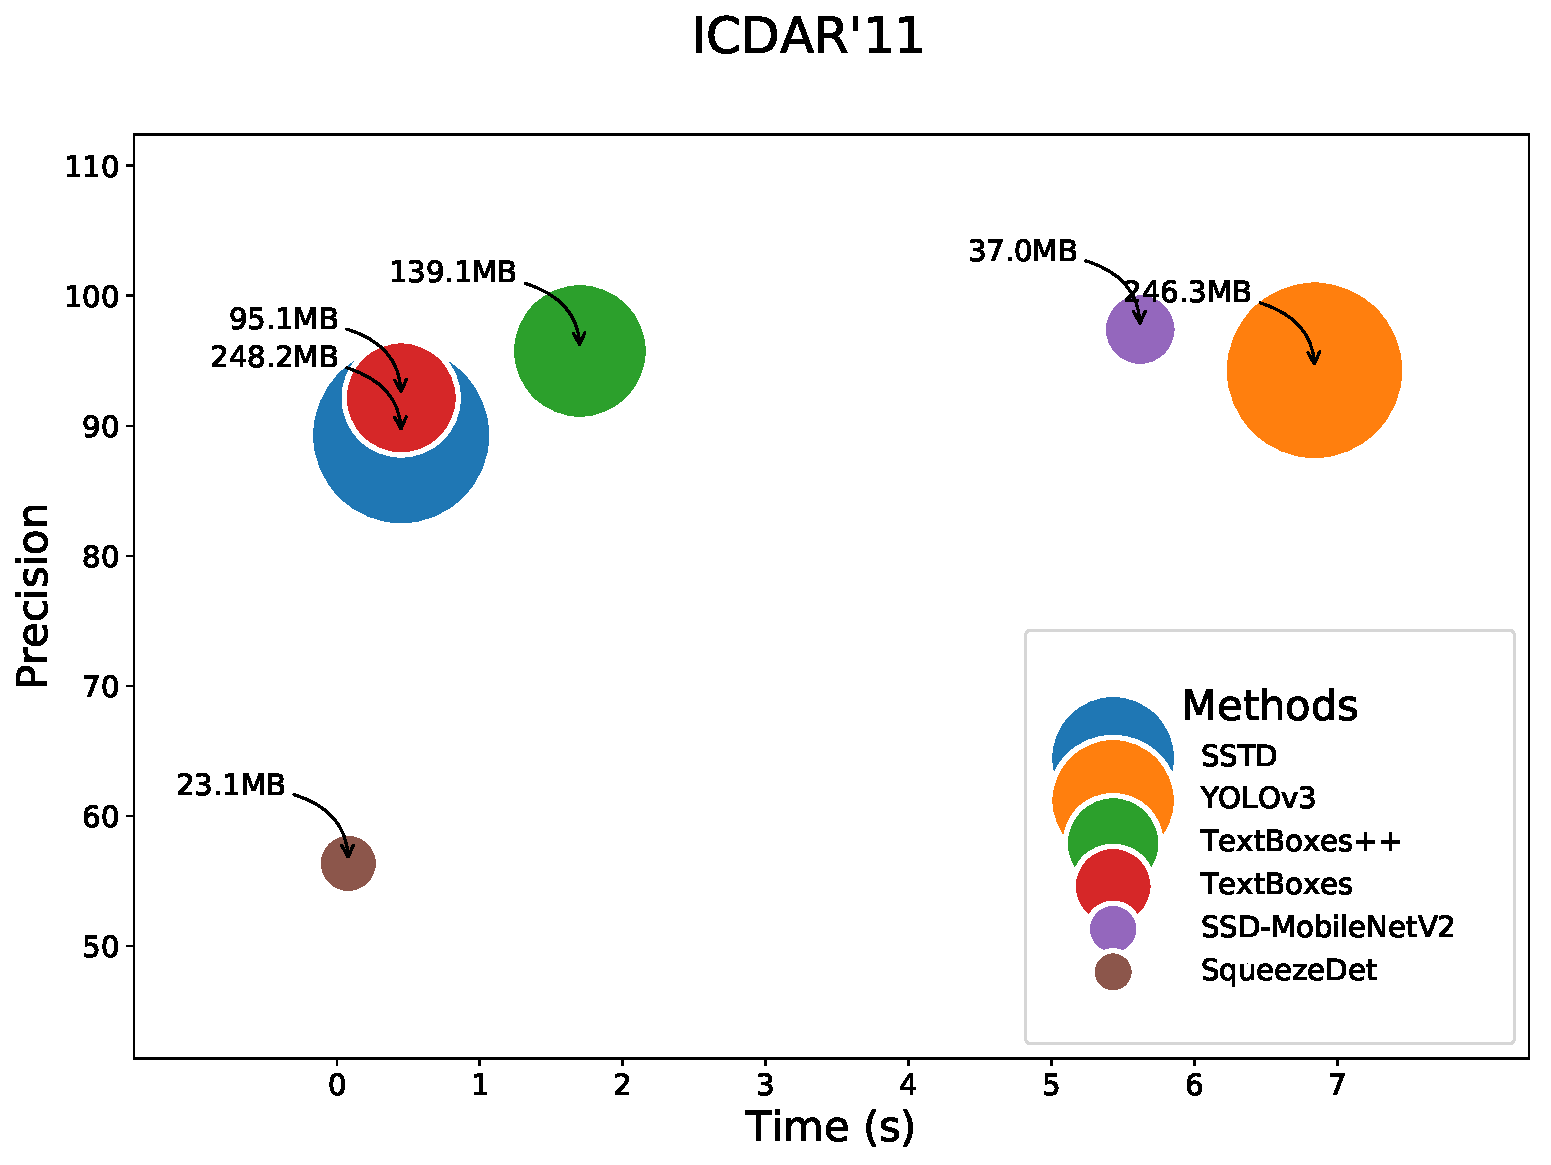
\includegraphics[height=0.25\textheight]{VISAPP/figs/efficacy-and-efficiency/deep-methods-icdar11-precision.pdf}
    % 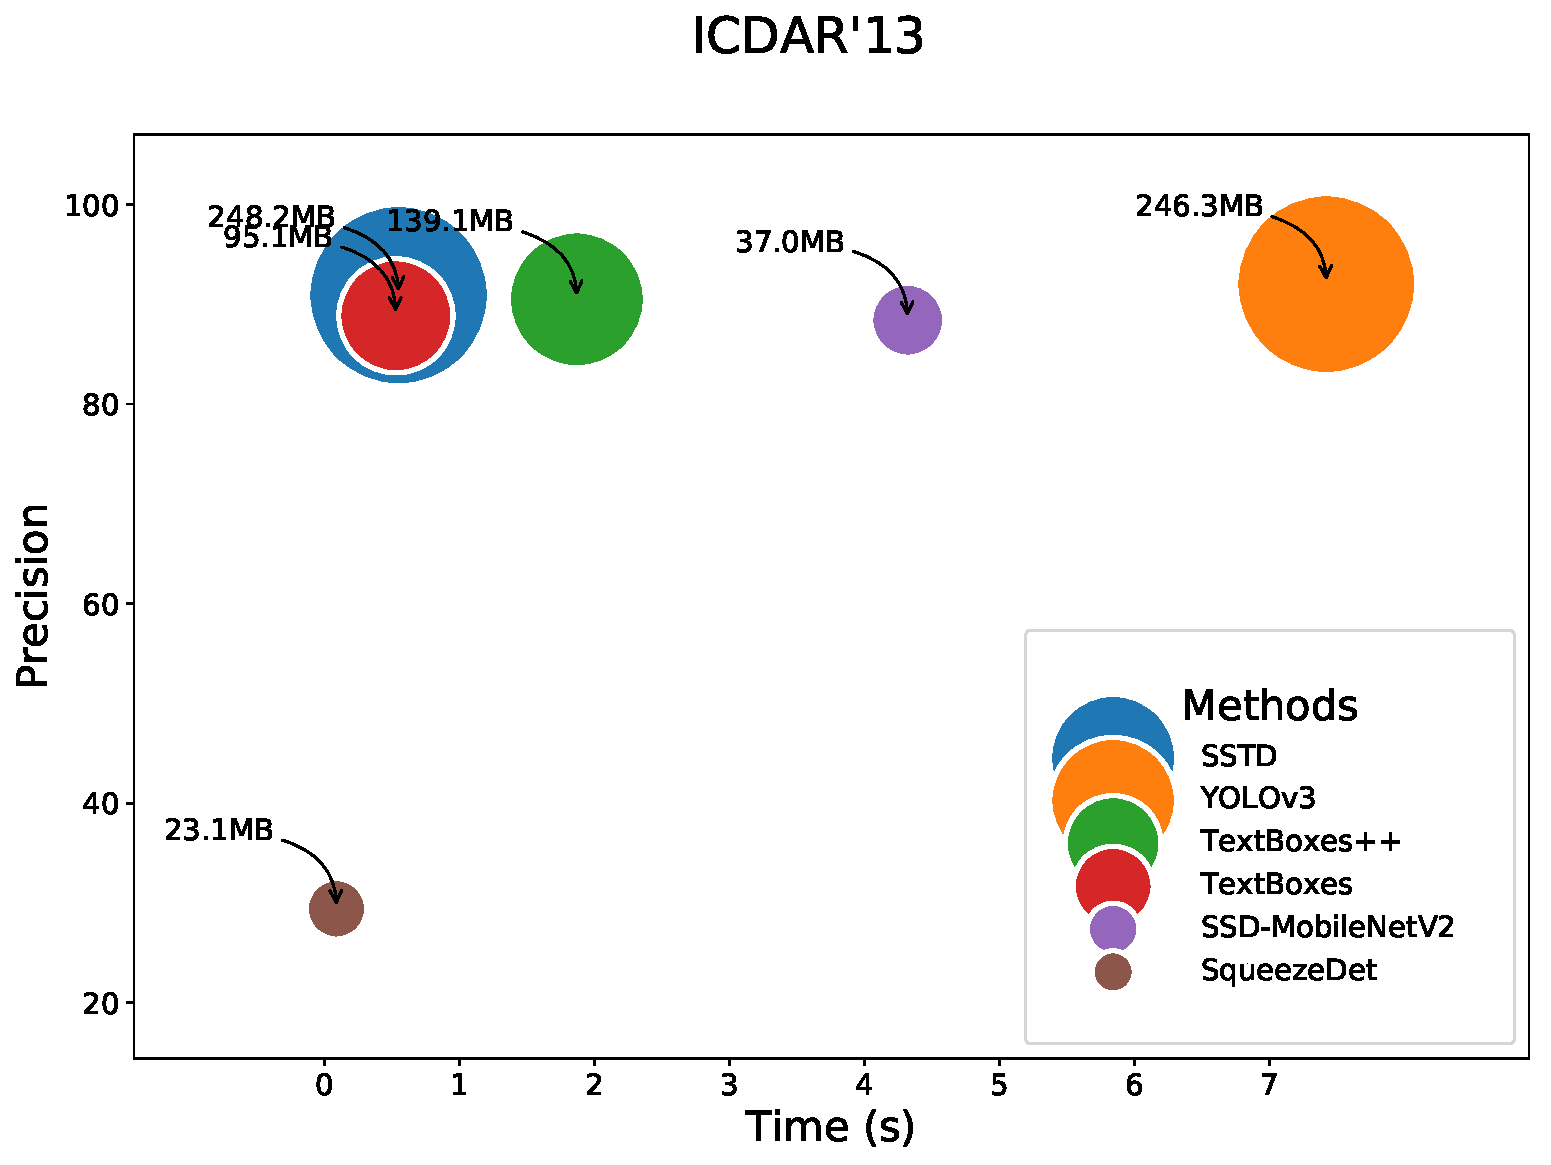
\includegraphics[height=0.25\textheight]{VISAPP/figs/efficacy-and-efficiency/deep-methods-icdar13-precision.pdf} \\
    % 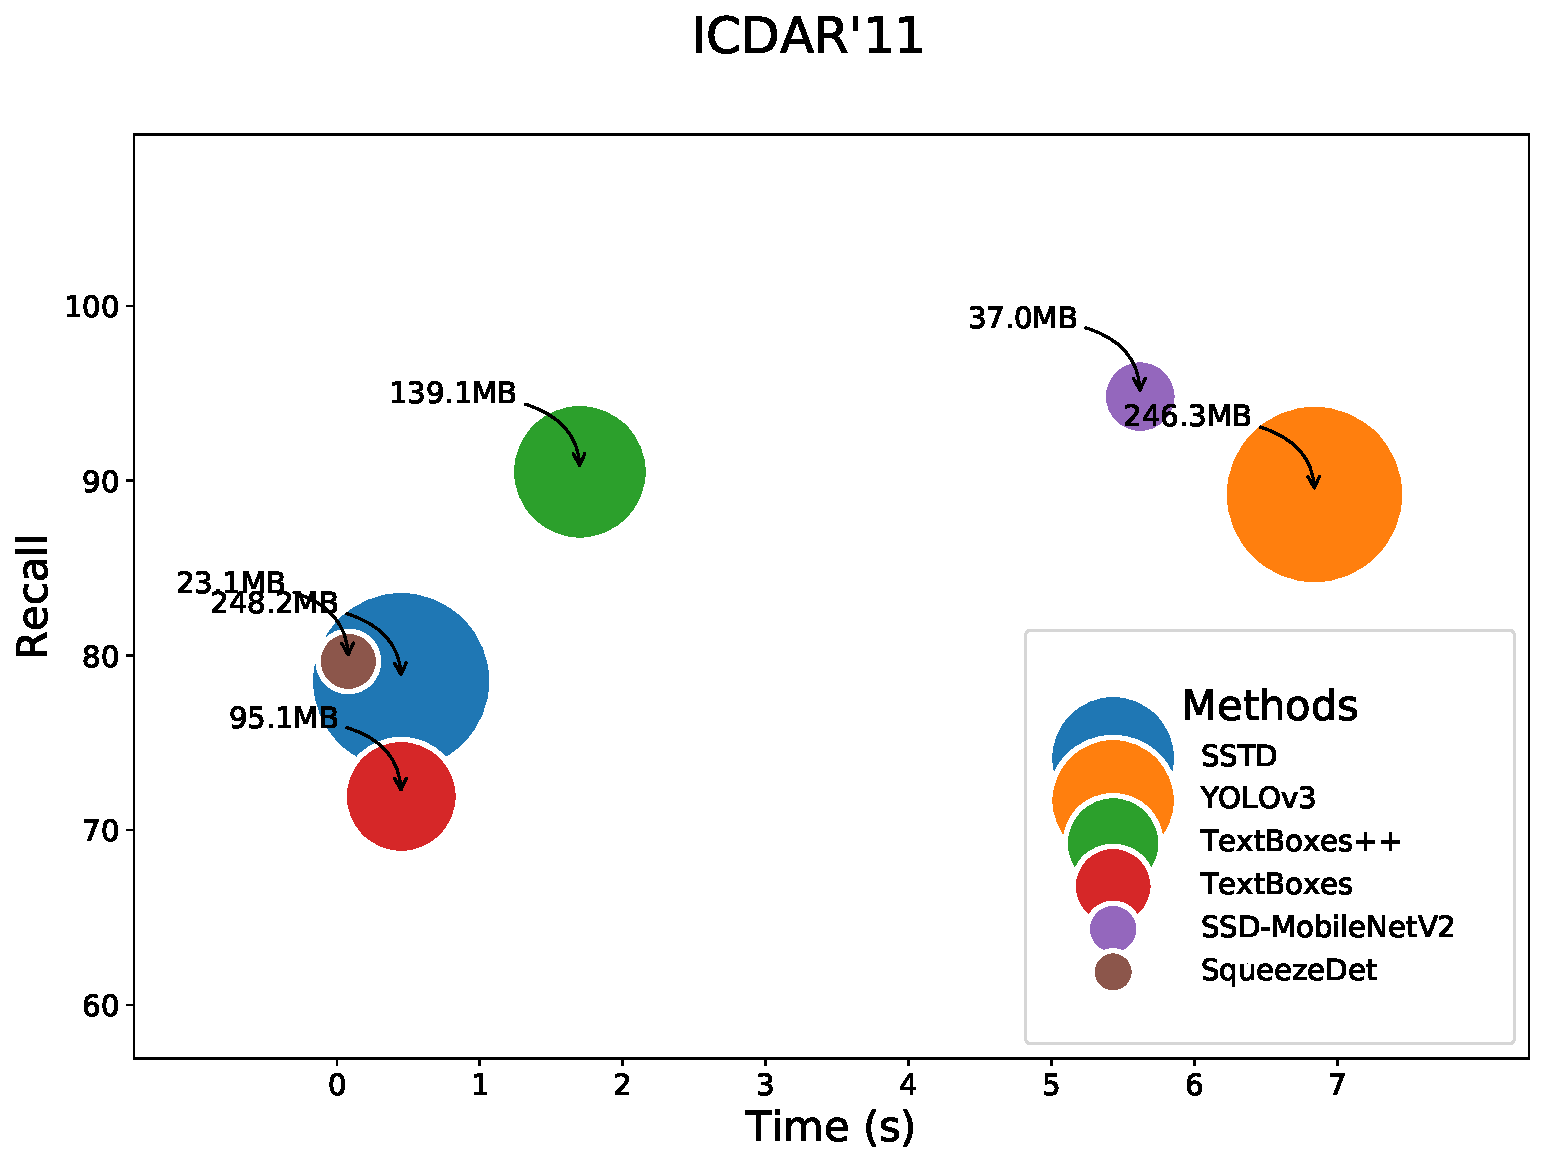
\includegraphics[height=0.25\textheight]{figs/efficacy-and-efficiency/deep-methods-icdar11-recall.pdf}
    % 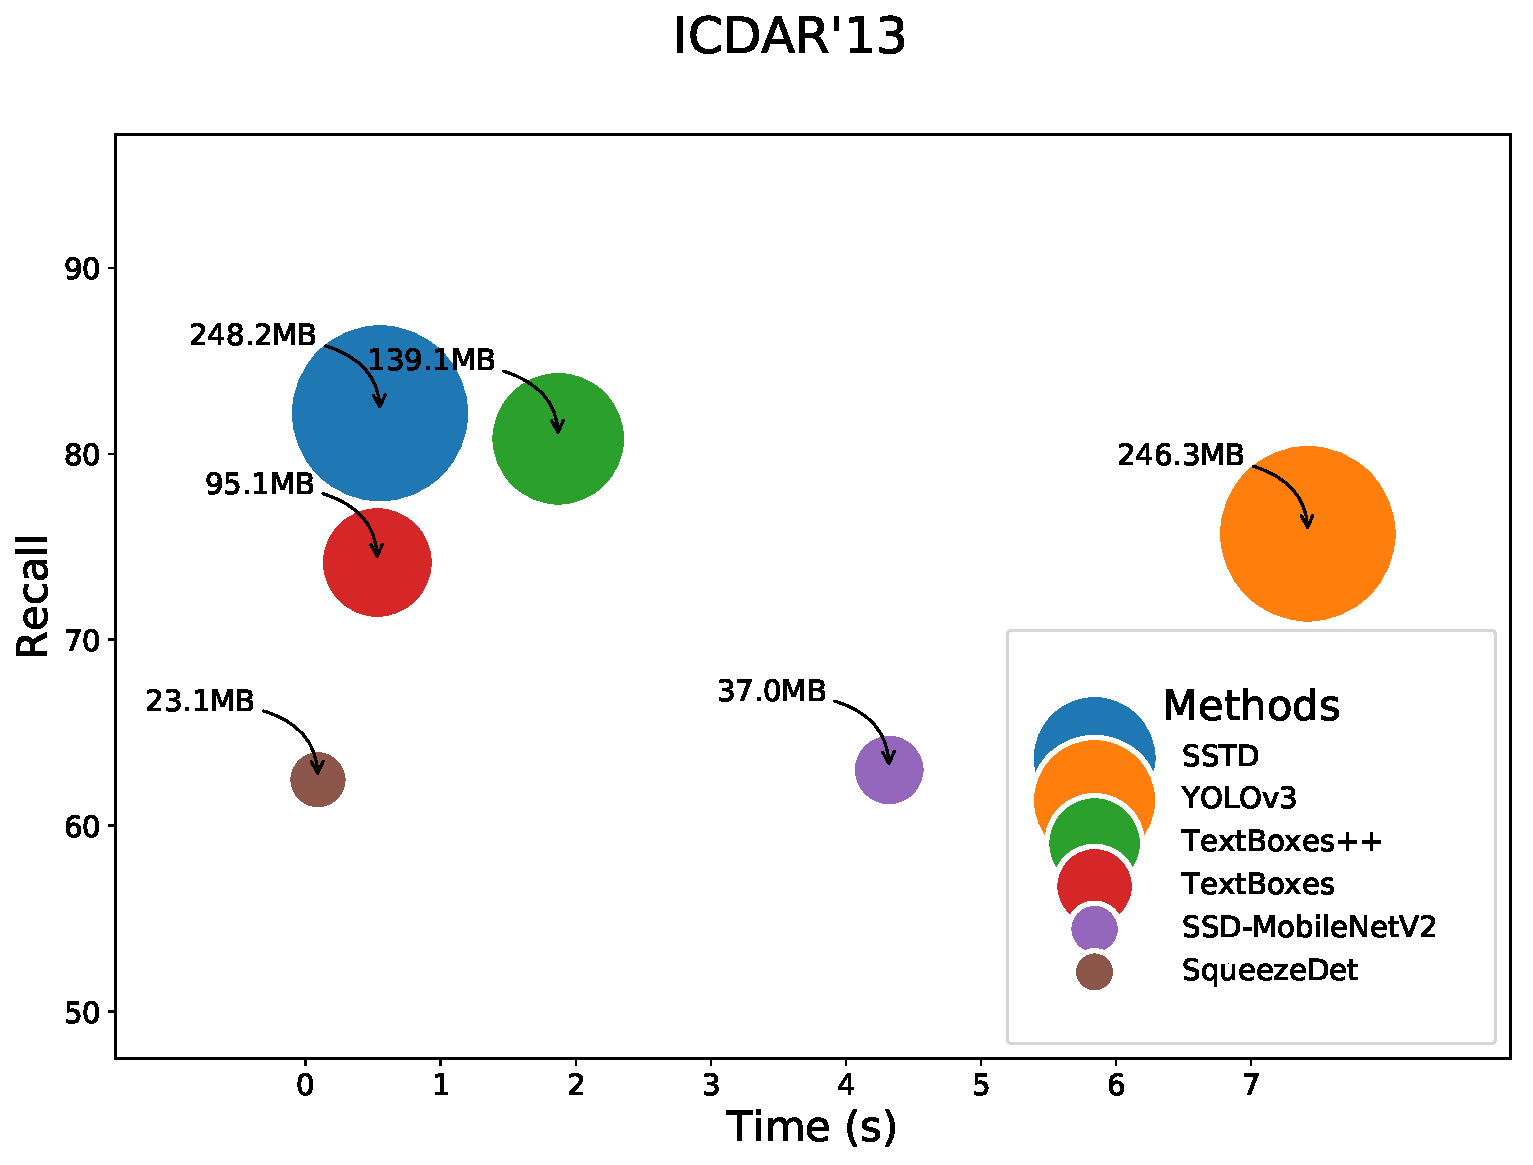
\includegraphics[height=0.25\textheight]{figs/efficacy-and-efficiency/deep-methods-icdar13-recall.pdf} \\
    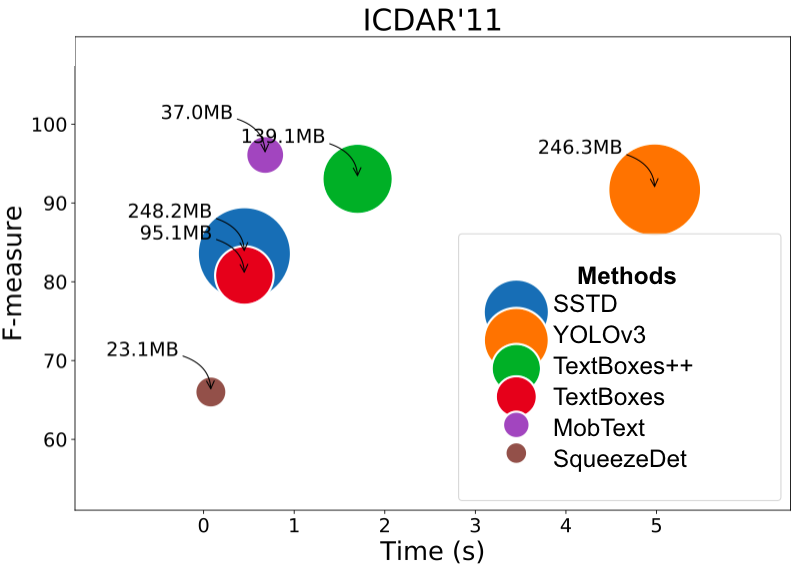
\includegraphics[width=0.80\textwidth]{ICIP_frankenstein/figs/deep-methods-icdar11-f-measure.png} \\
    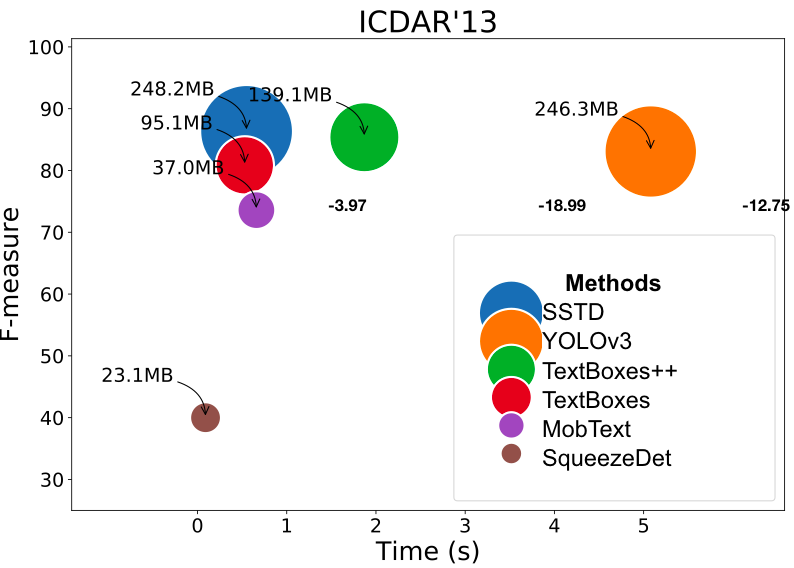
\includegraphics[width=0.80\textwidth]{ICIP_frankenstein/figs/deep-methods-icdar13-f-measure.png}
    \caption{Comparison results among the evaluated methods considering aspects of efficacy and efficiency.}
    \label{fig:deep-methods-efficacy-and-efficiency}
\end{figure}

%Now, we will turn our attention for 
In term of 
%evaluating 
the efficiency of the presented methods, 
Fig.~\ref{fig:deep-methods-efficacy-and-efficiency} summarizes the results considering the metrics used to assess the effectiveness of the evaluated methods, in terms of F-measure, along with the metrics for measuring the efficiency of those methods, considering the ICDAR'11 and ICDAR'13 datasets.

Regarding efficiency (processing time and disk usage), the proposed method (MobText) yielded very competitive results, taking only $0.45$ and $0.55$ seconds per image, considering the ICDAR'11 and ICDAR'13, respectively. Comparing MobText with the baseline methods originally proposed for text localization (TextBoxes, TextBoxes++, SSTD), the proposed method presented very competitive results with a processing time of $0.67$ seconds per image and with disk usage of about $37.0$MB. In contrast, the most effective baseline methods, the SSTD and TextBoxes++ networks, presented competitive results in terms of effectiveness and worse results in terms of processing time in comparison with the proposed method. Regarding the disk usage, MobText also presented the best balance between accuracy and model size.   

Now, when compared with the state-of-the-art approaches for object detection, the proposed method also presented competitive results. In this case, the fastest approach for text localization was the SqueezeDet network, which takes about $0.1$ seconds per image, on average. However, when we take into account the trade-off between efficiency and effectiveness, we can safely argue that the proposed method presented a better compromise between these two measures. Figure~\ref{fig:qualitative-results-good-11} provides some cases of success and Figure~\ref{fig:qualitative-results-bad-11} cases of failure of the proposed method for the ICDAR'11 and Figures~\ref{fig:qualitative-results-good-13} and~\ref{fig:qualitative-results-bad-13} for ICDAR'13 datasets. 


\begin{figure}[!h]
	\centering

    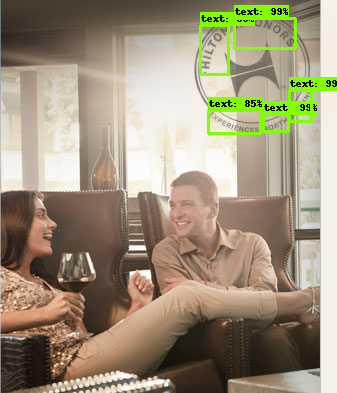
\includegraphics[height=0.29\textheight]{VISAPP/figs/qualitative-results/icdar11/69.png}
    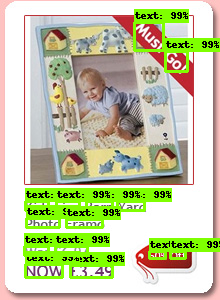
\includegraphics[height=0.29\textheight]{VISAPP/figs/qualitative-results/icdar11/46.png}
    
    \vspace{1.5mm}
    
    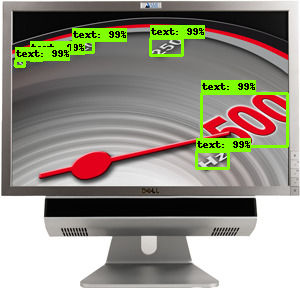
\includegraphics[height=0.20\textheight]{VISAPP/figs/qualitative-results/icdar11/14.png}
    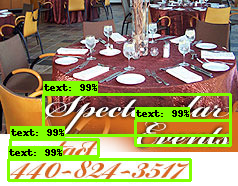
\includegraphics[height=0.20\textheight]{VISAPP/figs/qualitative-results/icdar11/29.png}
    
    \caption{Examples of success cases of the proposed approach for the ICDAR'11 dataset. Green bounding boxes indicate the regions correctly localized.}
	\label{fig:qualitative-results-good-11}
\end{figure}

%includegraphics[width=0.19\textwidth]{VISAPP/figs/qualitative-results/icdar11/117.png} \\

\begin{figure}[!h]
	\centering

    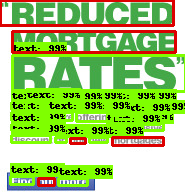
\includegraphics[height=0.20\textheight]{VISAPP/figs/qualitative-results/icdar11/22m.png}
    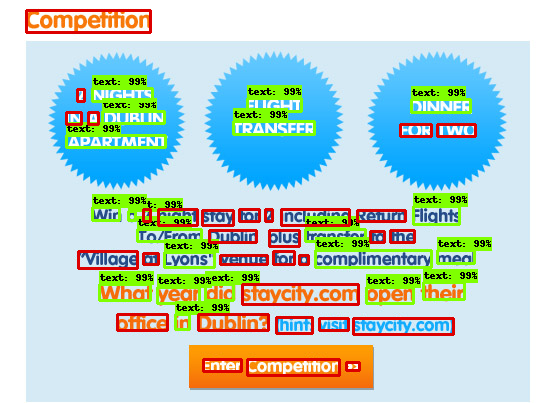
\includegraphics[height=0.20\textheight]{VISAPP/figs/qualitative-results/icdar11/53m.png}

    \vspace{1.5mm}

    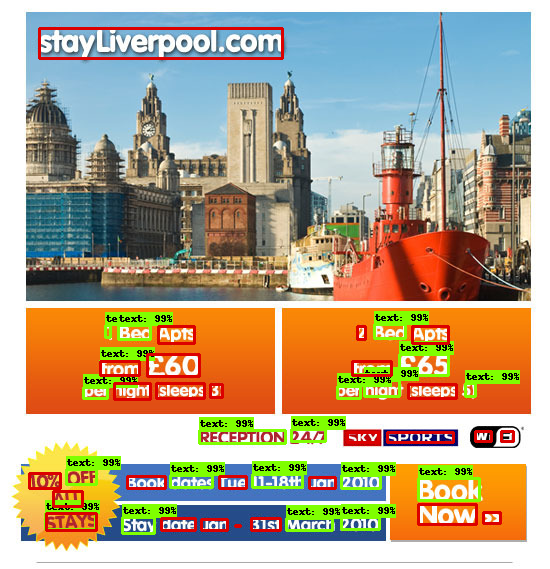
\includegraphics[height=0.25\textheight]{VISAPP/figs/qualitative-results/icdar11/32m.png}
    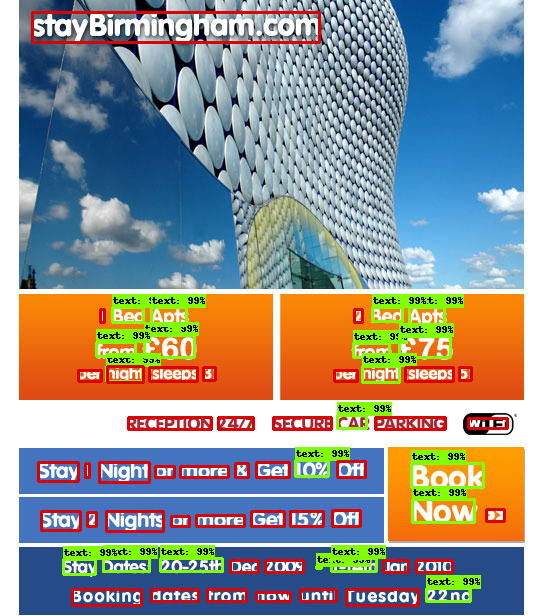
\includegraphics[height=0.25\textheight]{VISAPP/figs/qualitative-results/icdar11/10m.png}

\caption{Examples of failure cases of the proposed approach for the ICDAR'11 dataset. Green bounding boxes indicate the regions correctly localized, while red bounding boxes show candidate regions not detected by our method.}
	\label{fig:qualitative-results-bad-11}
\end{figure}

\begin{figure}[!h]
	\centering

    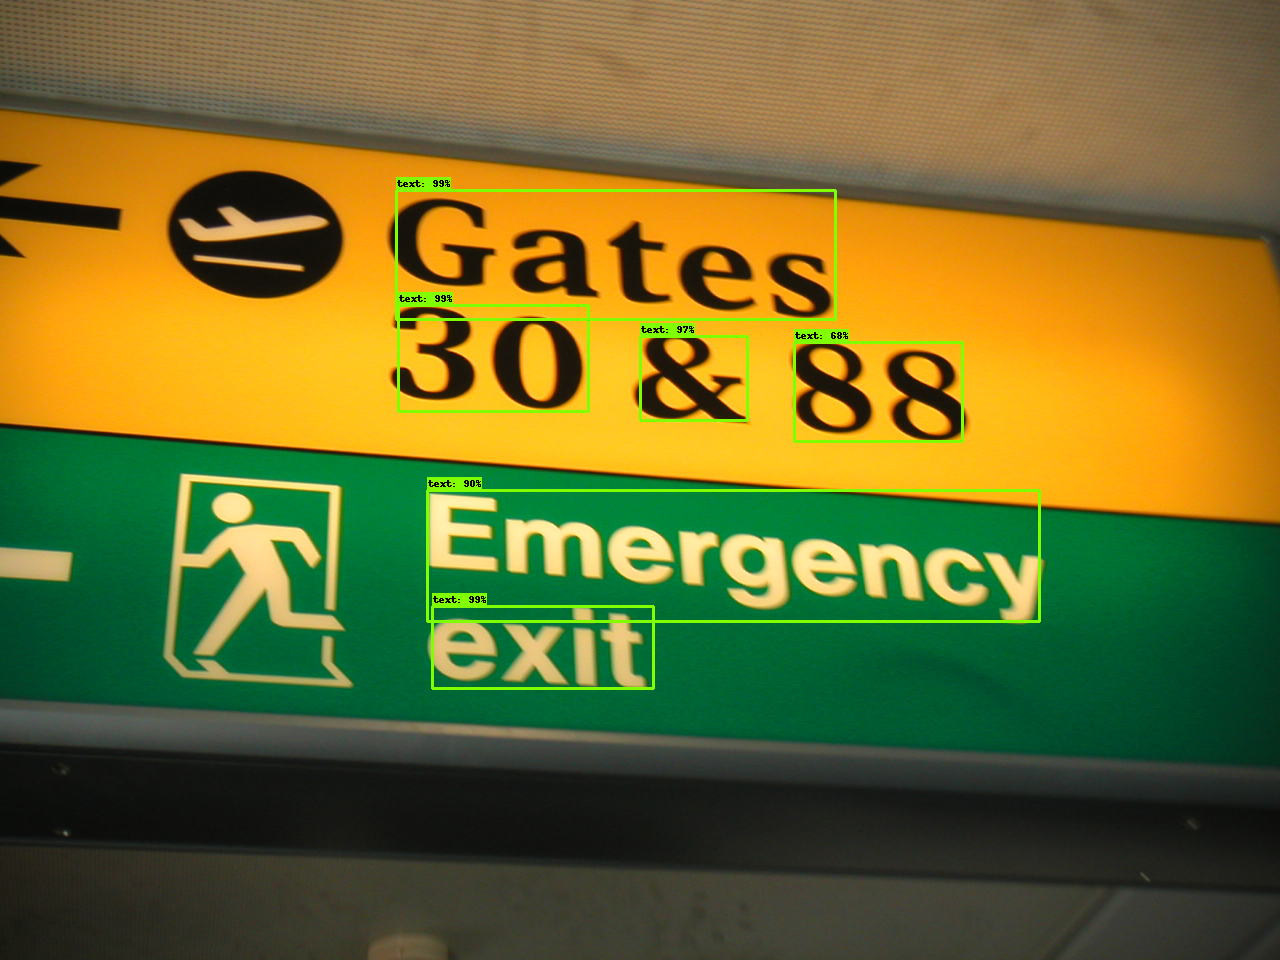
\includegraphics[height=0.20\textheight]{VISAPP/figs/qualitative-results/icdar13/19.png}
    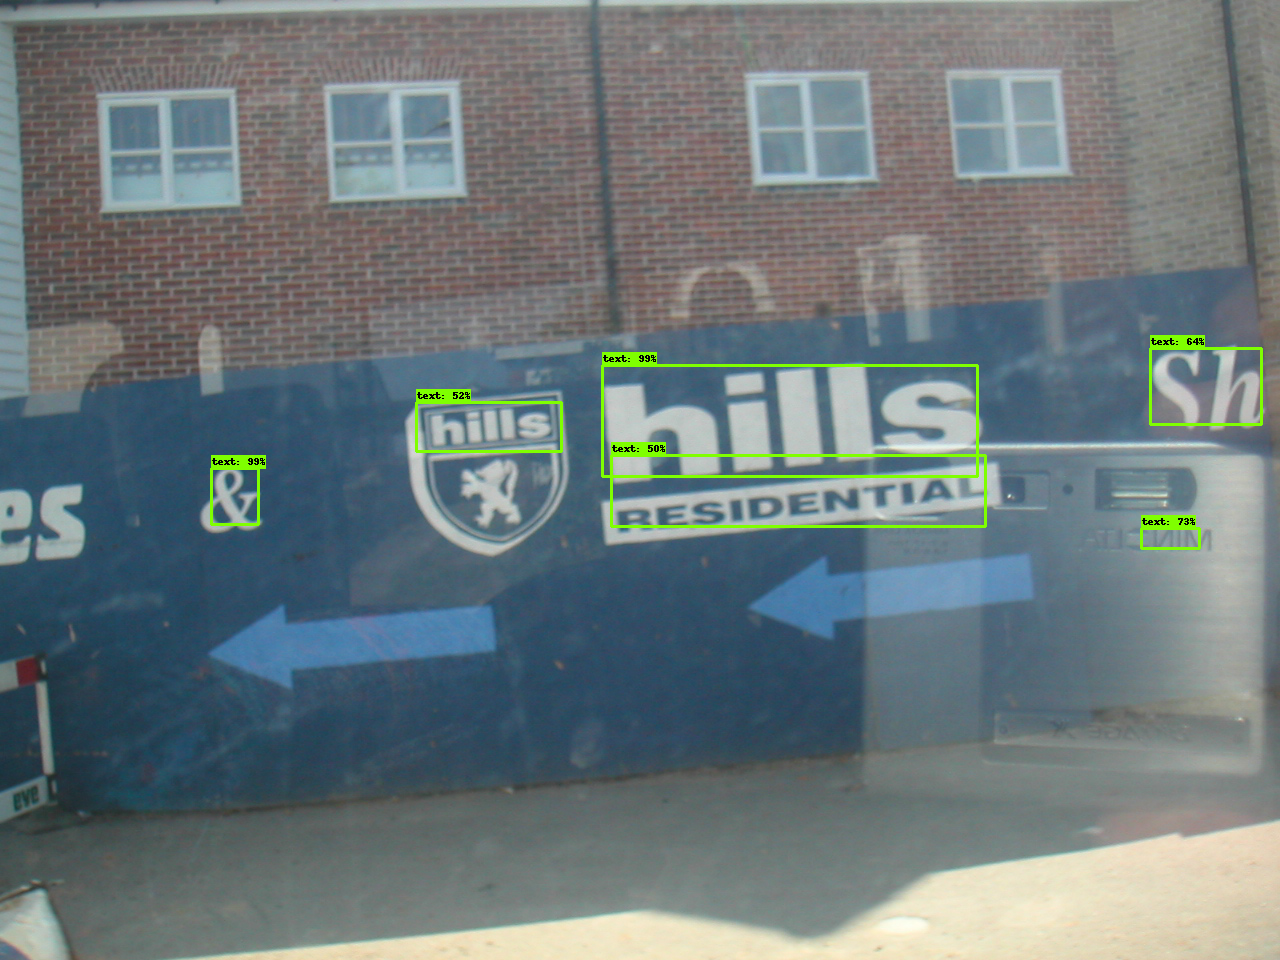
\includegraphics[height=0.20\textheight]{VISAPP/figs/qualitative-results/icdar13/83.png}
    
    \vspace{1.5mm}
    
    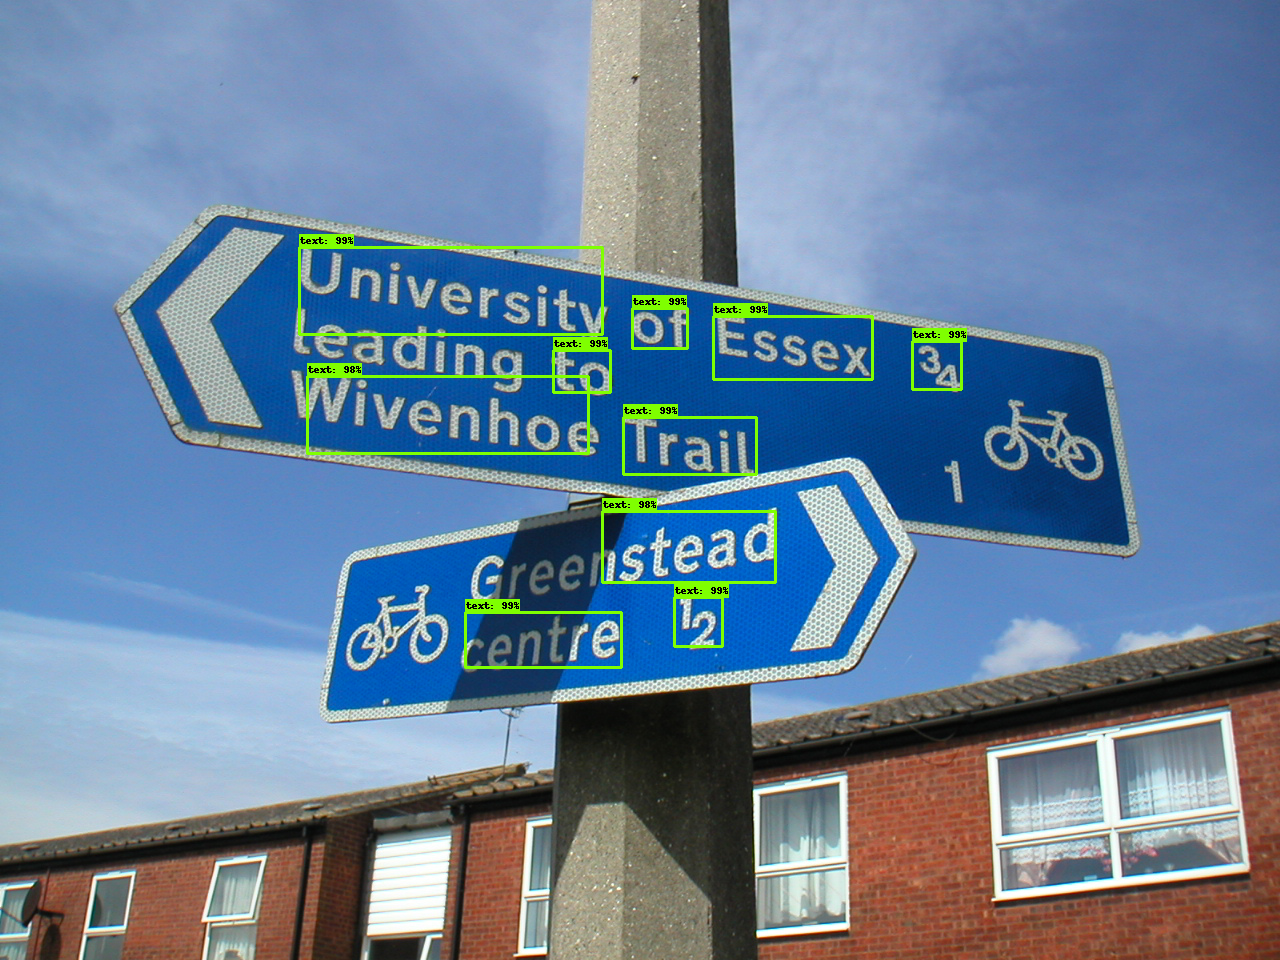
\includegraphics[height=0.20\textheight]{VISAPP/figs/qualitative-results/icdar13/129.png}
    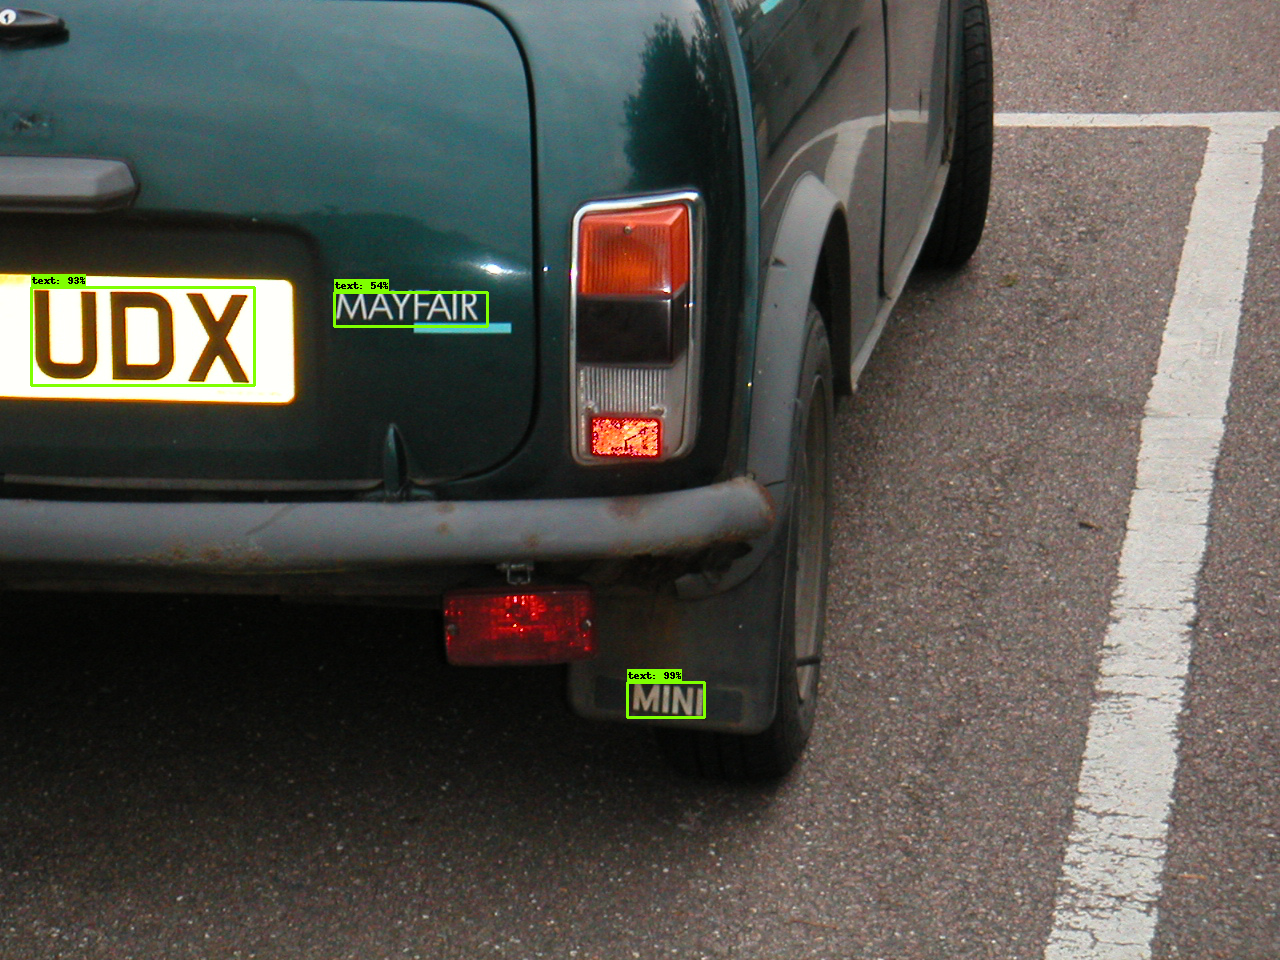
\includegraphics[height=0.20\textheight]{VISAPP/figs/qualitative-results/icdar13/140.png}
	\caption{Examples of success cases of the proposed approach for the ICDAR'13 dataset. Green bounding boxes indicate the regions correctly localized.}
	\label{fig:qualitative-results-good-13}
\end{figure}
\begin{figure}[!h]
	\centering
    
    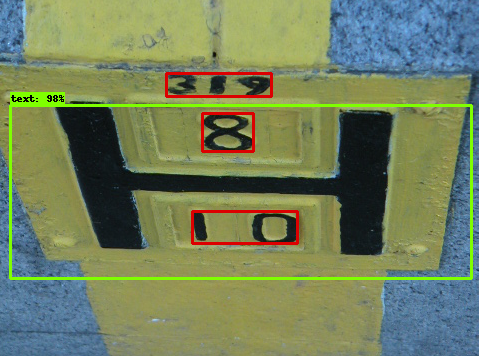
\includegraphics[height=0.20\textheight]{VISAPP/figs/qualitative-results/icdar13/1m_crop.png}
    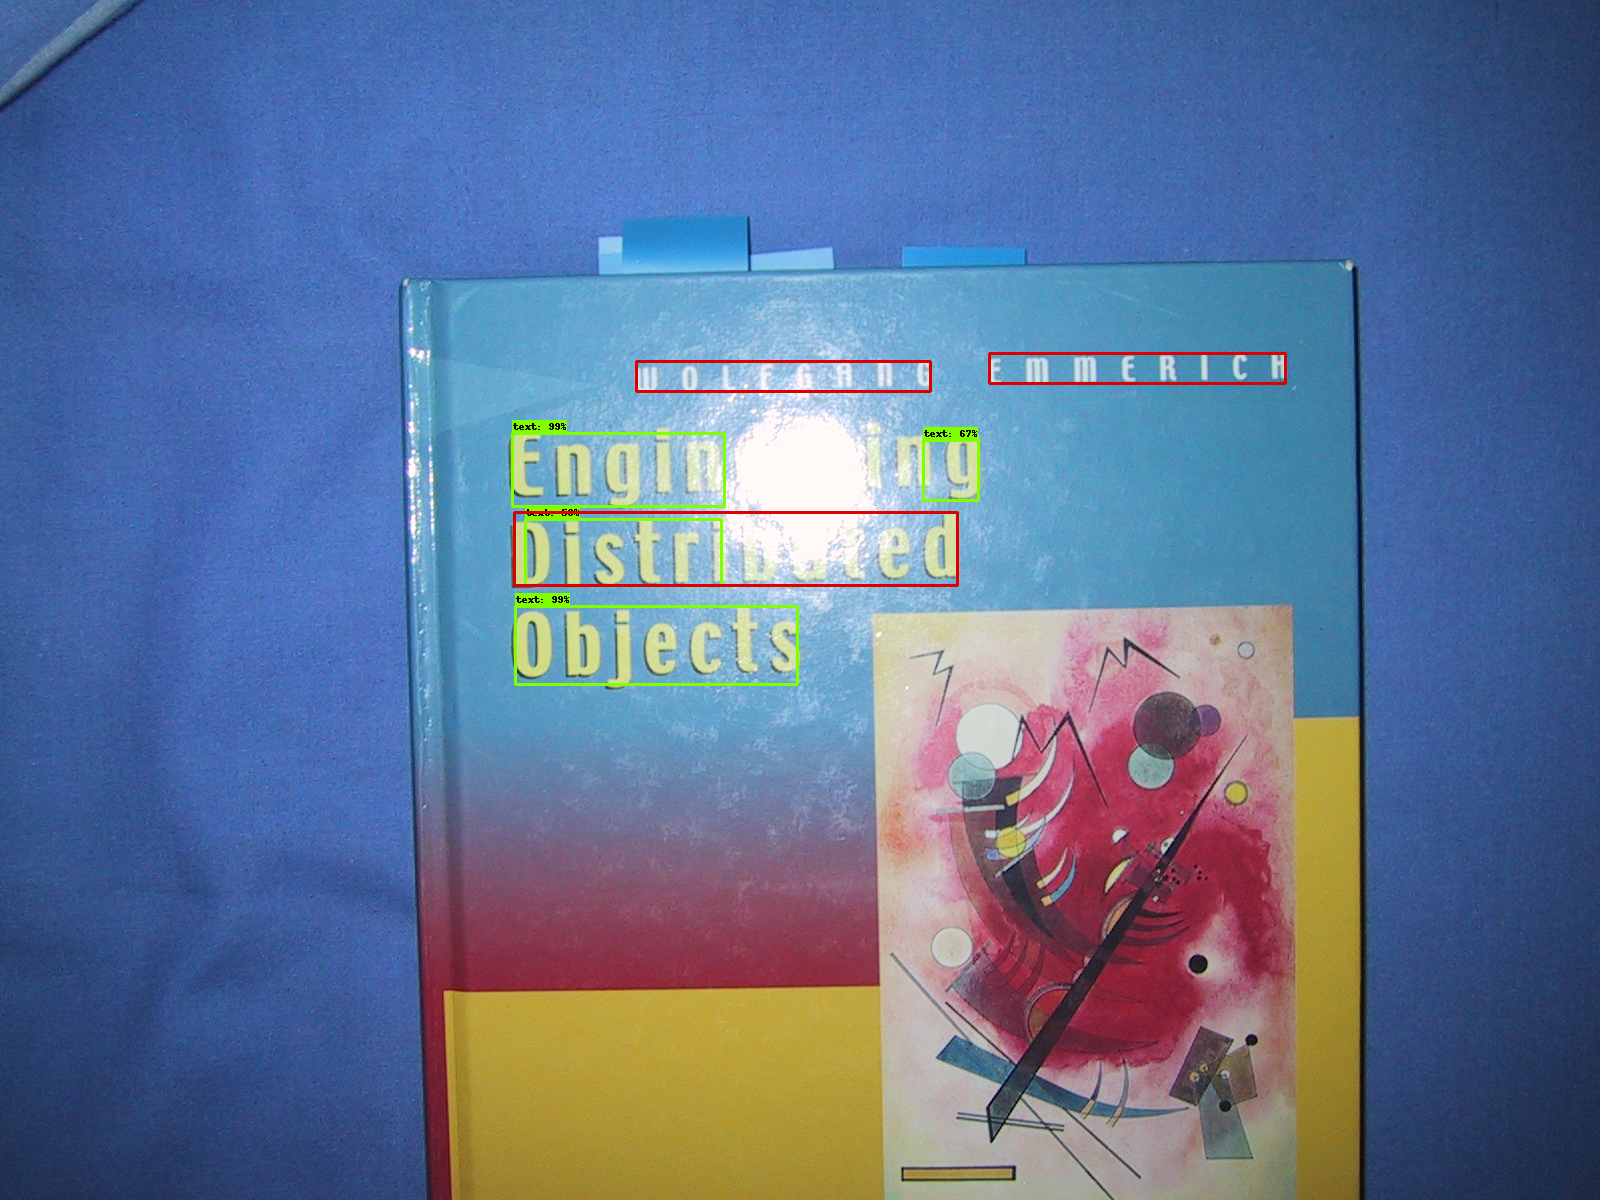
\includegraphics[height=0.20\textheight]{VISAPP/figs/qualitative-results/icdar13/18m.png}

    \vspace{1.5mm}

    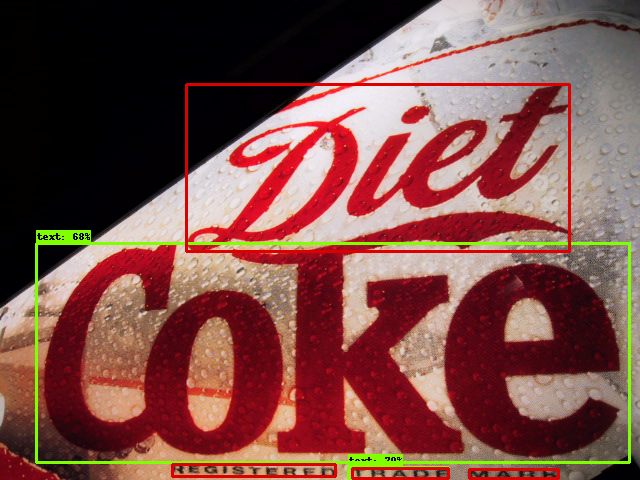
\includegraphics[height=0.20\textheight]{VISAPP/figs/qualitative-results/icdar13/41m.png}
    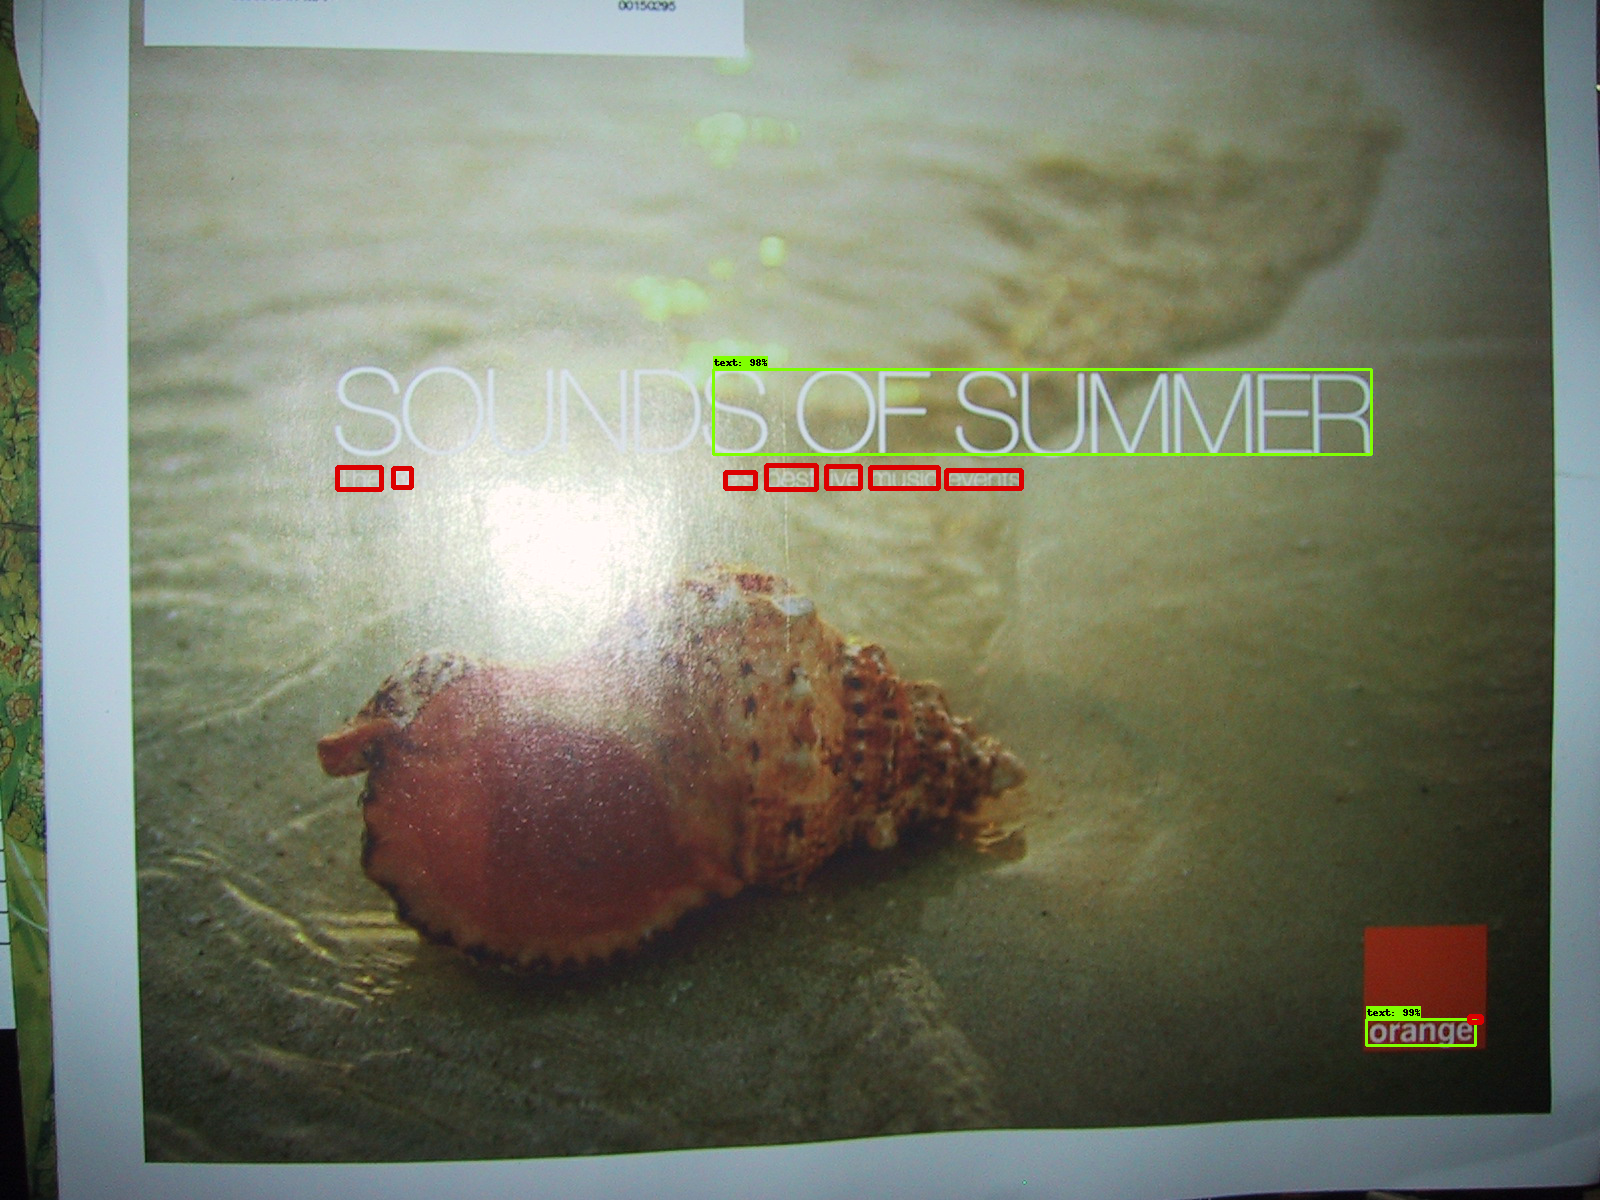
\includegraphics[height=0.20\textheight]{VISAPP/figs/qualitative-results/icdar13/48m.png}
%   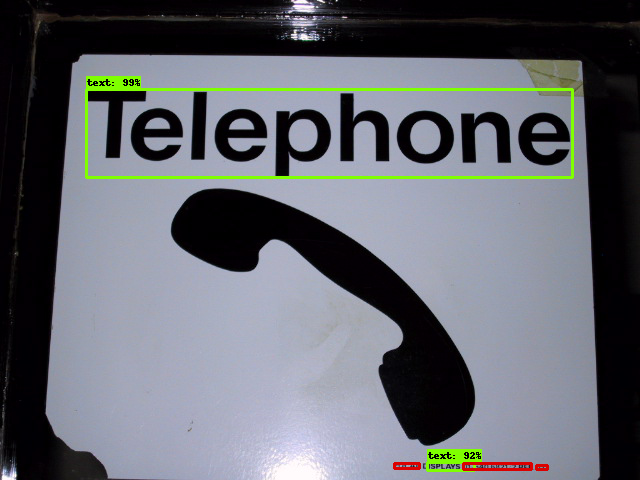
\includegraphics[height=0.20\textheight]{VISAPP/figs/qualitative-results/icdar13/49m.png}

	\caption{Examples of failure cases of the proposed approach for the ICDAR'13 dataset. Green bounding boxes indicate the regions correctly localized, while red bounding boxes show candidate regions were not detected by our method.}
	\label{fig:qualitative-results-bad-13}
\end{figure}

The proposed method is able to detect multi-oriented texts and even texts with textured backgrounds. However, as we could observe, the proposed approach presented some difficulties in localizing scene text in the ICDAR'13 dataset. In comparison with results achieved for the ICDAR'11, the precision and recall rates decreased $9.36$ and $31.61$ percentage points, respectively, which suggest that our network did not localized several candidate regions containing texts.

\begin{figure}[!h]
    \centering
    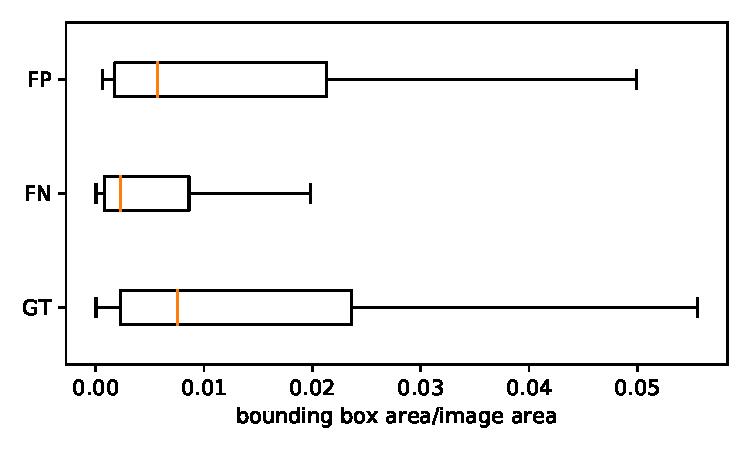
\includegraphics[width=0.75\textwidth]{VISAPP/figs/boxplot_error_icdar13.pdf}
    \caption{Comparison among distributions of relative areas of bounding boxes from Ground-Truth (GT), False Negatives (FN) cases, and False Positive (FP) cases. We omitted the points considered outliers for a better visualization.}
    \label{fig:boxplot}
\end{figure}

To understand the reasons that led the proposed method to have this difficult in localizing text for the ICDAR'13 datasets, we performed an analysis of failure cases taking into account the relative area of missed bounding boxes. Figure~\ref{fig:boxplot} presents a box-plot graph that shows the distribution of the relative area of bounding boxes (i.e., ratio of bounding box area to image area) for the ground-truth, false positive cases, and false negative cases.

\begin{figure}[!h]
    \centering
    %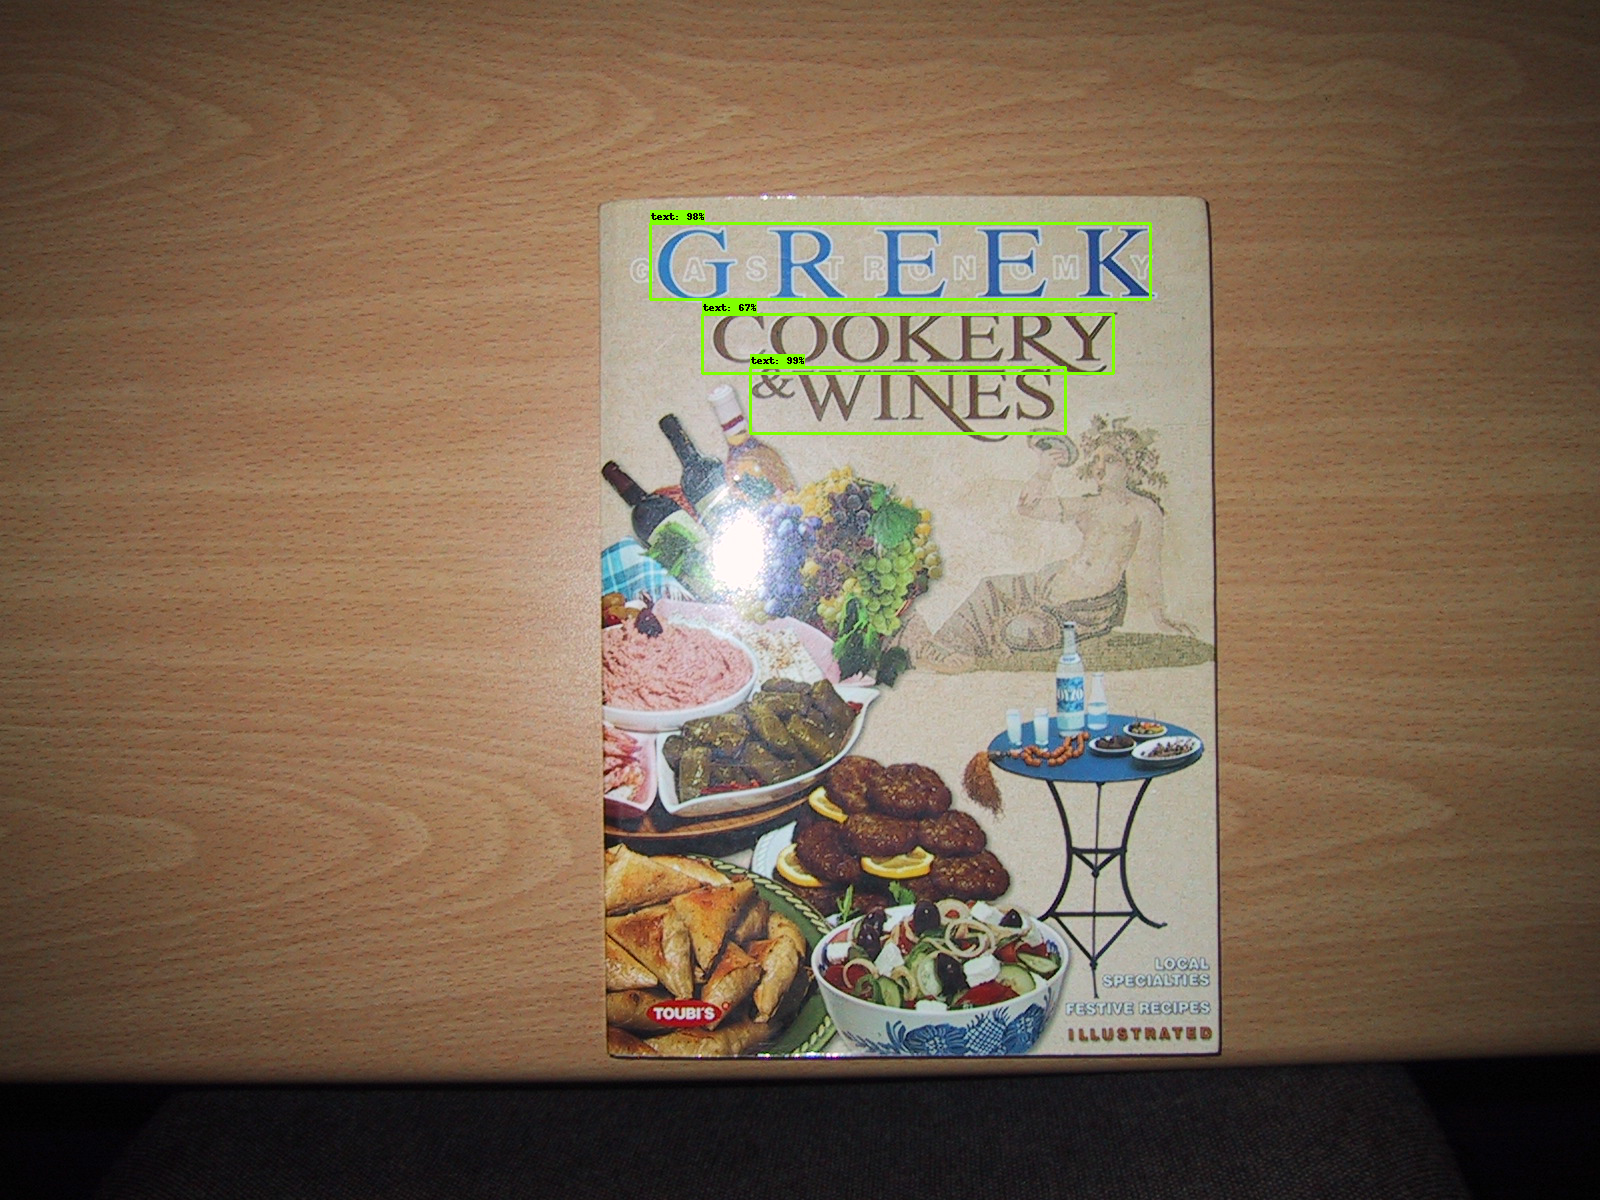
\includegraphics[width=\columnwidth]{version-2/figs/small_box.jpg}
    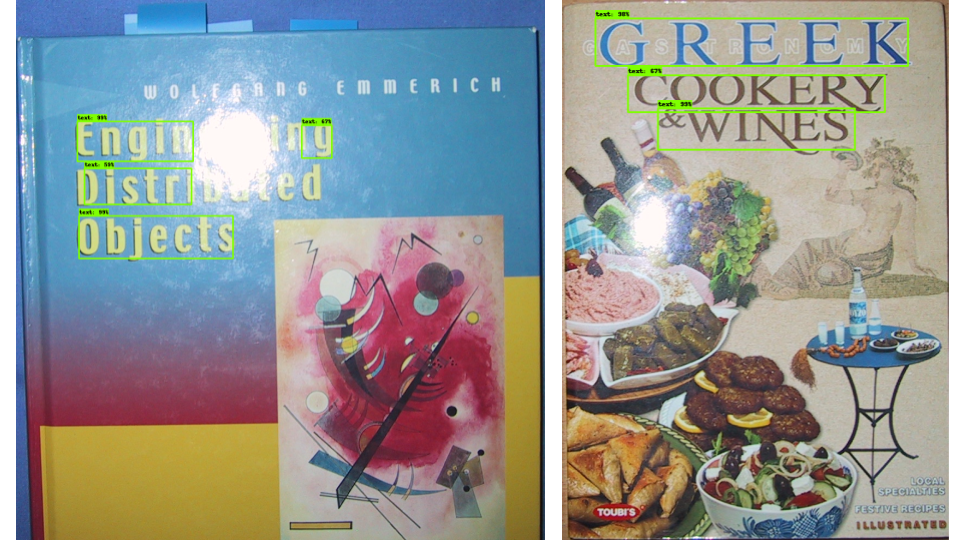
\includegraphics[width=0.99\textwidth]{VISAPP/figs/hires_samples.png}
    \caption{Two high resolution examples of ICDAR'13 dataset with both medium-sized text (detected by our method) and small-sized (not detected).}
    \label{fig:small_example}
\end{figure}

As we can observe, the missed bounding boxes (false negative cases) have a small relative area. More precisely, $75\%$ of false negative cases (third quartile of FN box-plot) have a relative area up to $0.01$ and correspond to $50\%$ of the bounding box present in the ground-truth (median of GT box-plot). This results suggest to us that high resolution images with relatively small text (see Fig.~\ref{fig:small_example}) are specially challenging to our method. To overcome this limitation, future investigations can be conducted to devise an architecture to better localize bounding boxes with multiple scales such as Feature Pyramid Networks (FPNs), as proposed by \citep{Lin2017CVPR}.

\subsection{Results on Mobile-Oriented Environment}

In terms of precision, recall, and F-Measure on ICDAR'11 and ICDAR'13 datasets, the proposal achieved the same results as on the non-restrictive scenario. Table~\ref{tab:times_dataset} shows the efficiency of the network in terms of inference time on both datasets. 

\begin{table}[!h]
    \centering
    \caption{Processing time of the embedded application on ICDAR datasets.}
    \label{tab:times_dataset}
    \begin{tabular}{lrrr}
        \toprule
        \ml{2}{*}{\textbf{Dataset}} & \mcol{3}{c}{\textbf{Processing Time (ms)}}  \\ 
                                    & \textbf{Min.} &  \textbf{Max.} &  \textbf{Average} \\ 
        \midrule
        ICDAR'11                    & $420$         & $524$          & $464$           \\ \hline
        ICDAR'13                    & $449$         & $602$          & $523$           \\
        
       \bottomrule
    \end{tabular}
\end{table}

As we are unable to evaluate the method in a quantitative manner regarding effectiveness on the images captured in the wild, the proposed solution was only evaluated in terms of efficiency, in processing time. A qualitative analysis was performed by taking into account the visual results of the detection on the images. 

 The average time of inference in $250$ images was $425$ms, with a minimum inference time of $343$ms and a maximum of $584$ms.


%%%%%%%%%%%%%%%%%
\begin{figure}[h!]
\centering
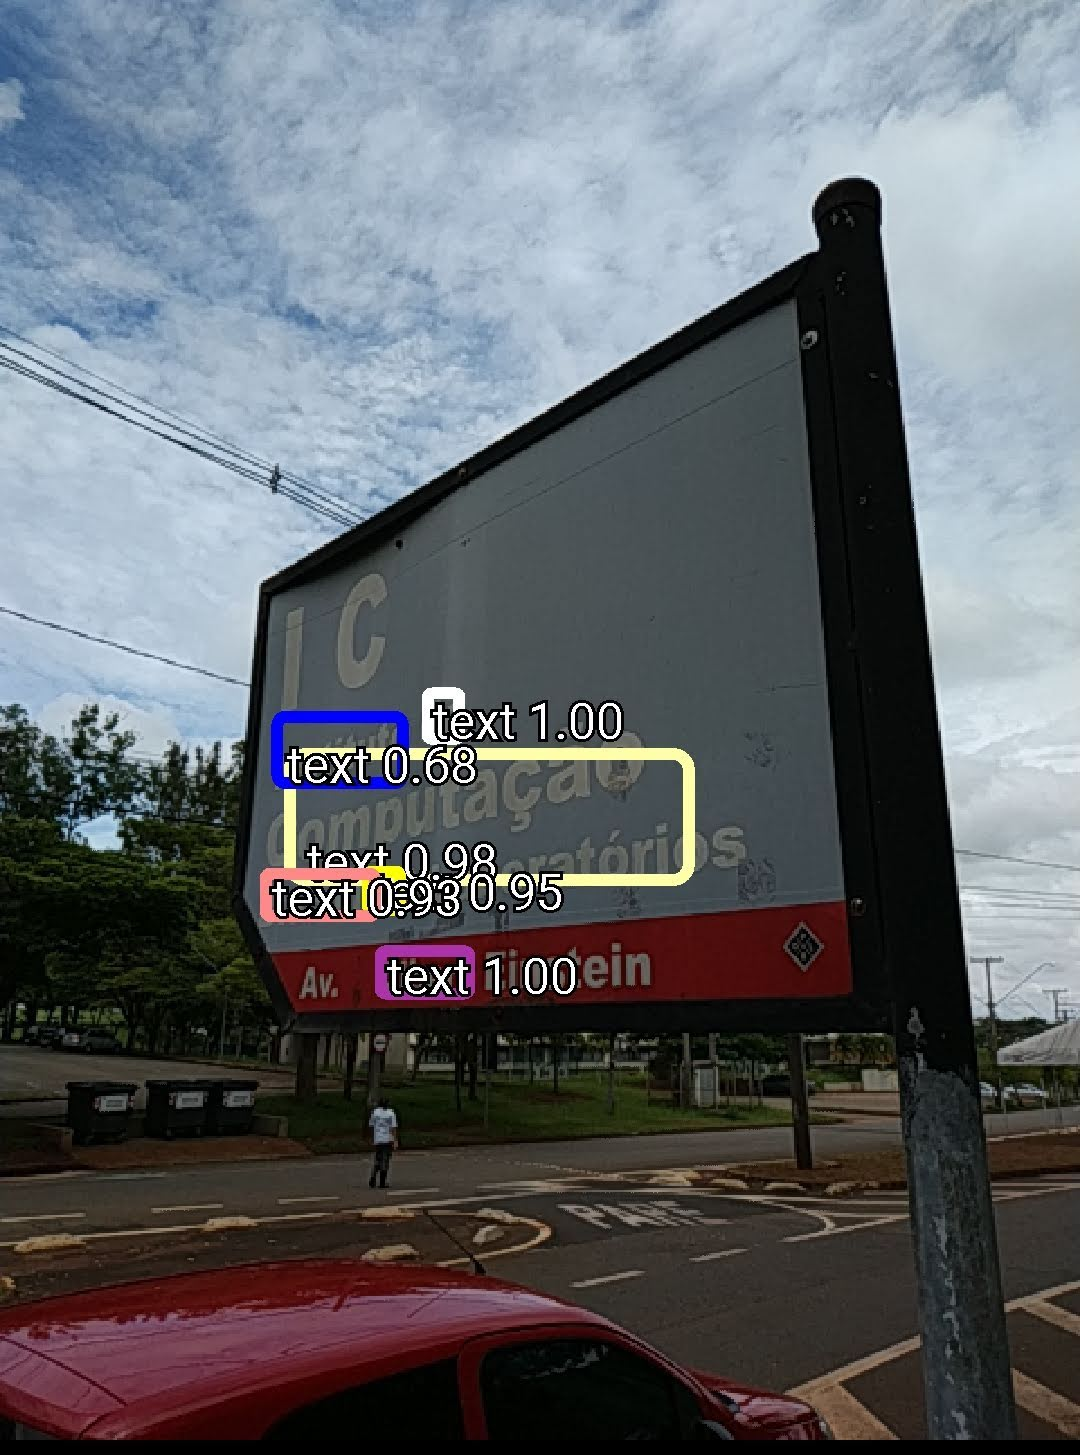
\includegraphics[width=0.49\textwidth]{Mobile/images/app27.jpg}
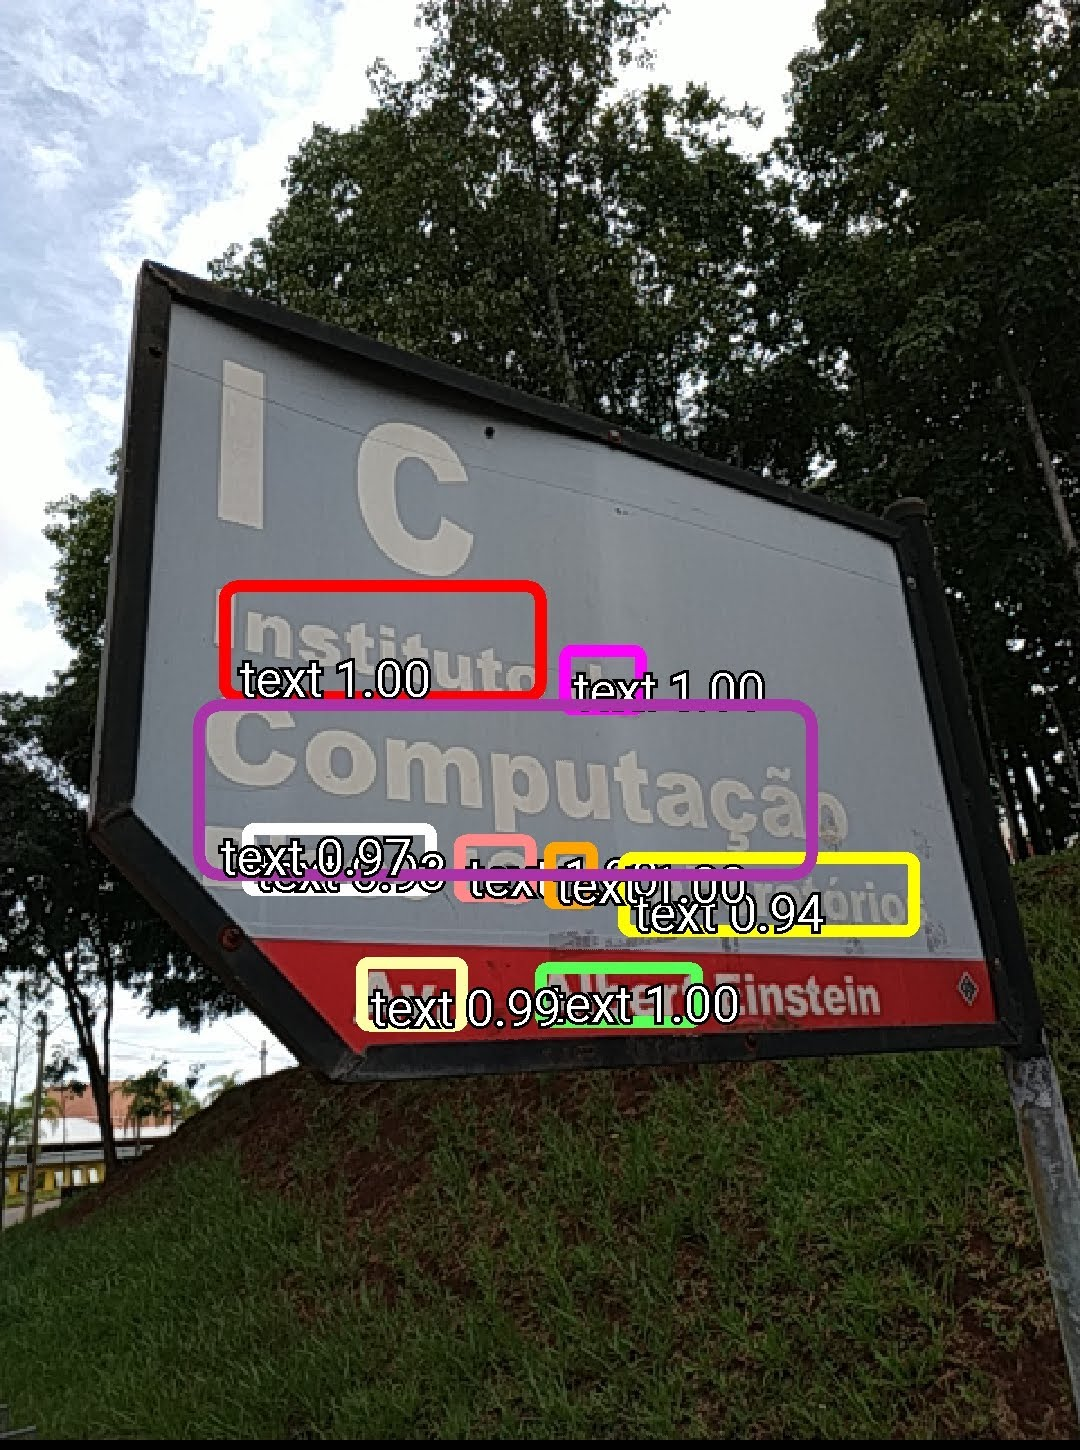
\includegraphics[width=0.49\textwidth]{Mobile/images/app28.jpg}

\caption{Example of scene text images captured with a perspective.}
\label{fig:ic-perspective}
\end{figure}
%%%%%%%%%%%%%%%%%%
Figure~\ref{fig:ic-perspective} shows the effect of the capturing angle of the texts in scene text images. As the system was only trained with horizontal aligned text, this kind of perspective lowers the system effectiveness.


\begin{figure}[h!]
\centering
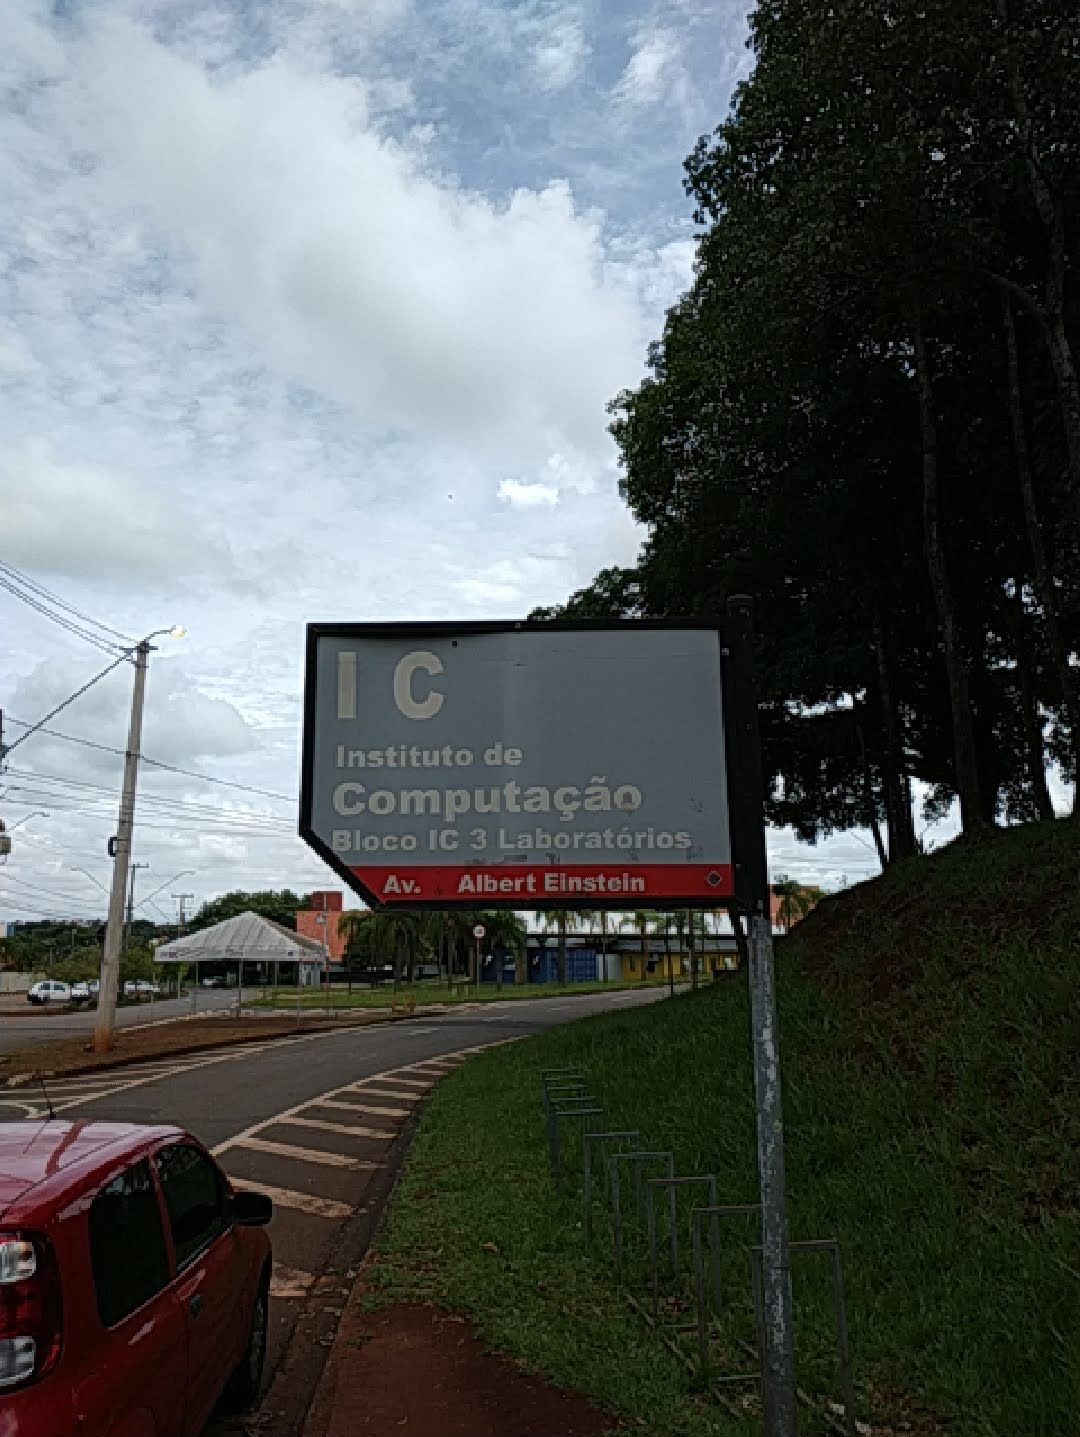
\includegraphics[width=0.49\textwidth]{Mobile/images/app24.jpg}
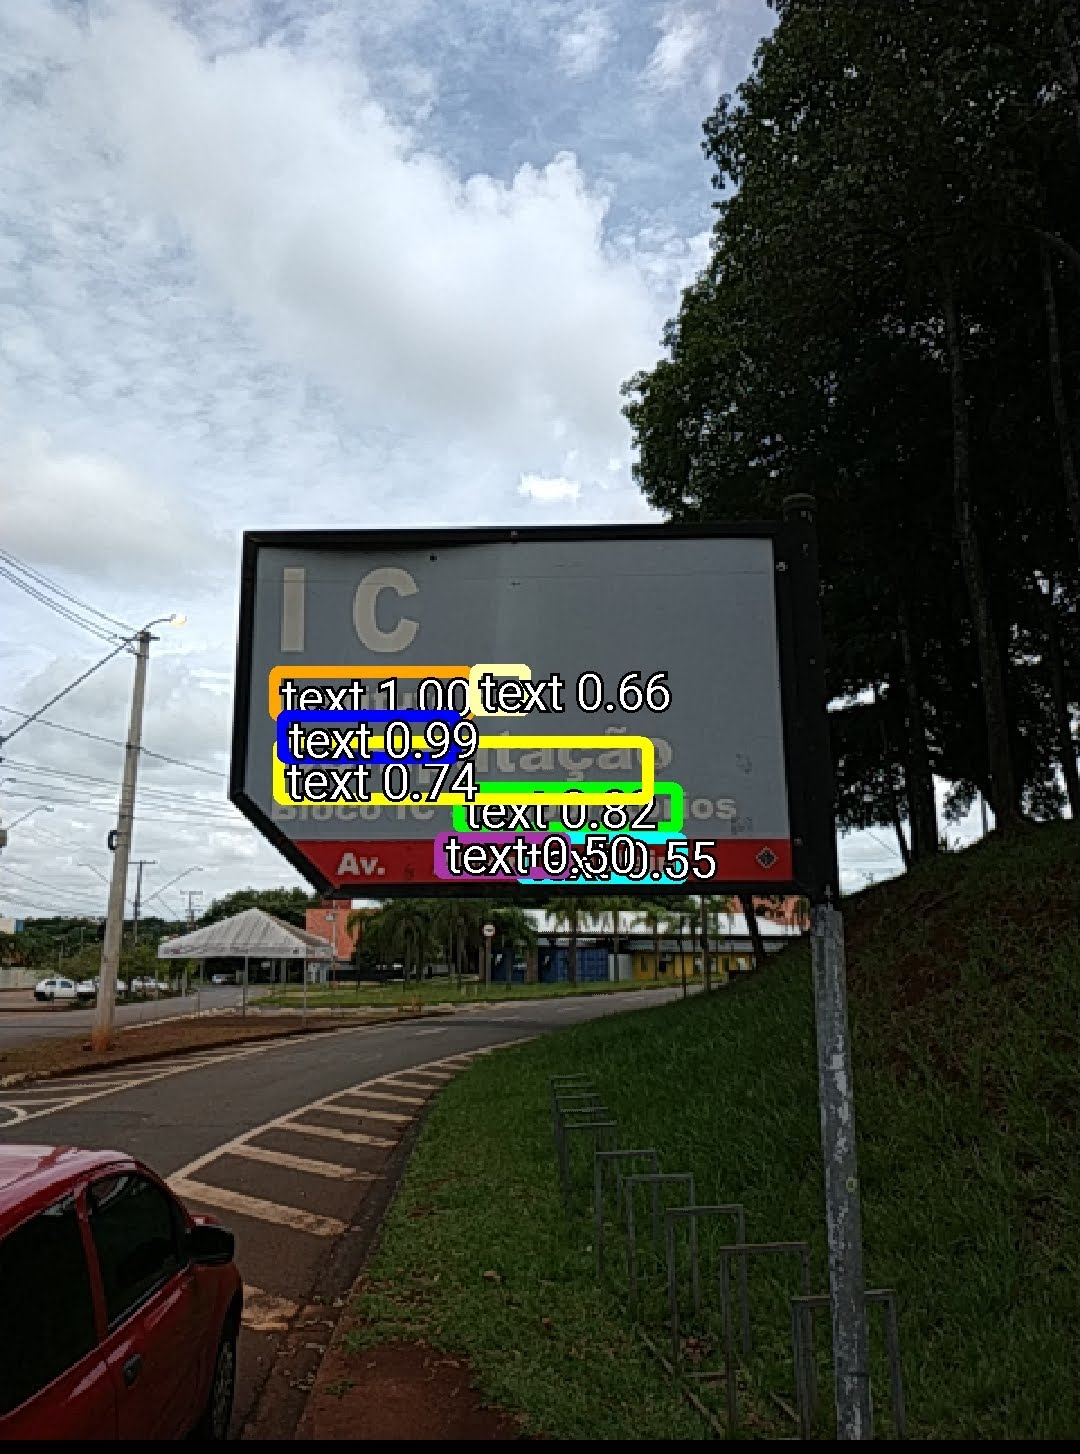
\includegraphics[width=0.49\textwidth]{Mobile/images/app25.jpg}

\vspace{1.5mm}

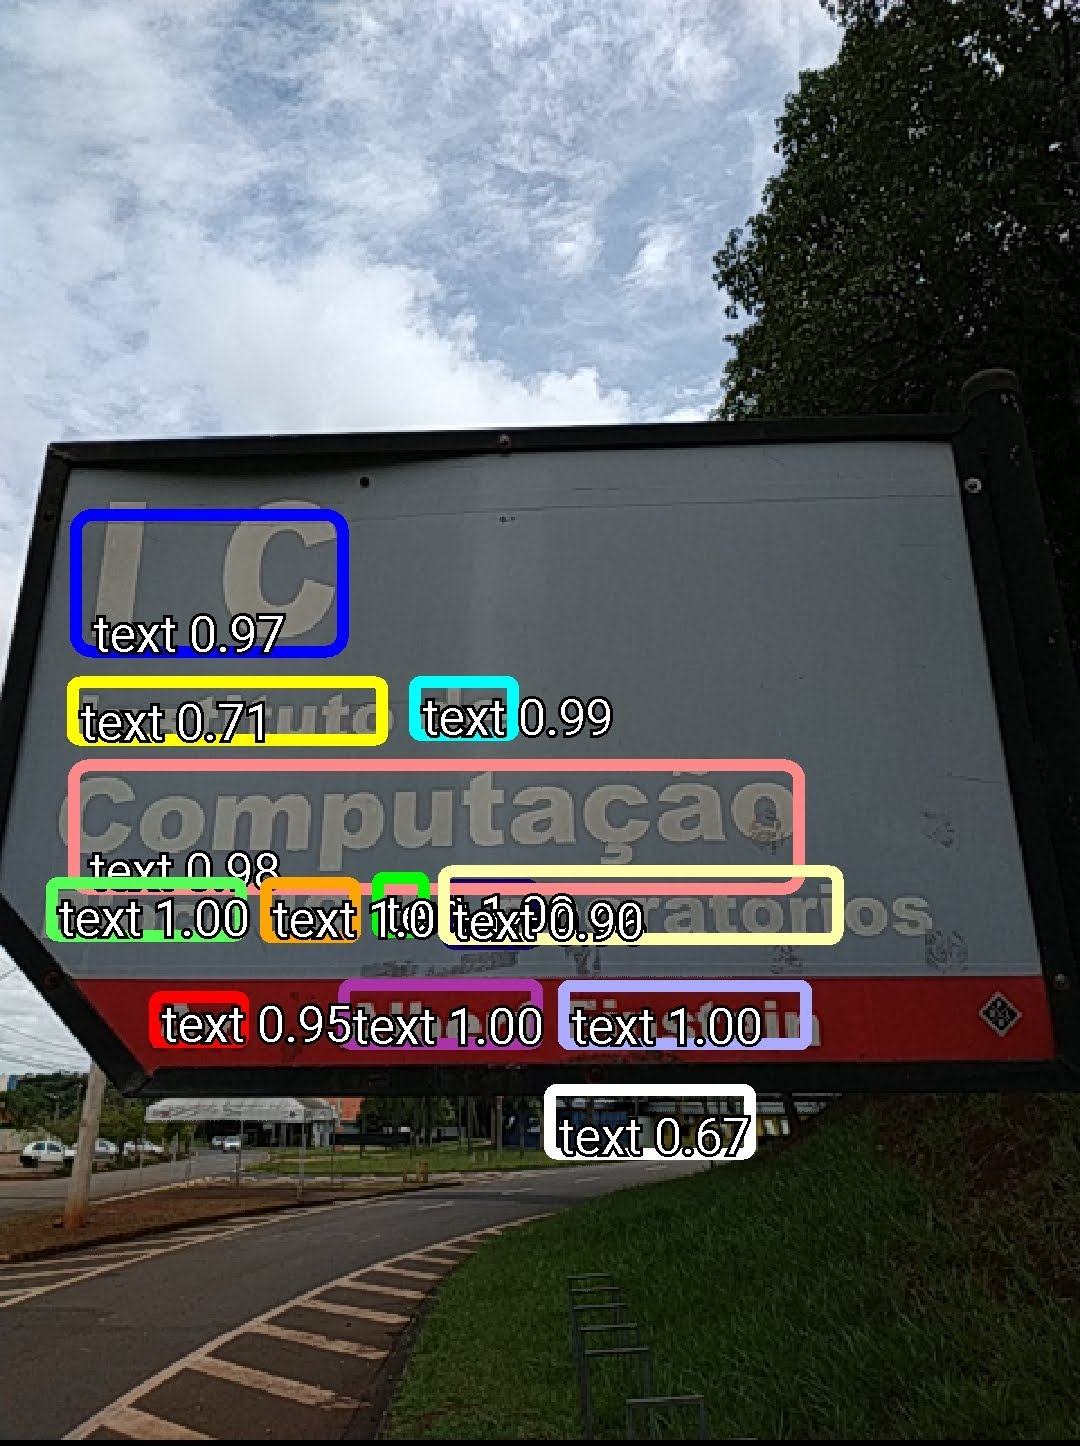
\includegraphics[width=0.49\textwidth]{Mobile/images/app23.jpg}
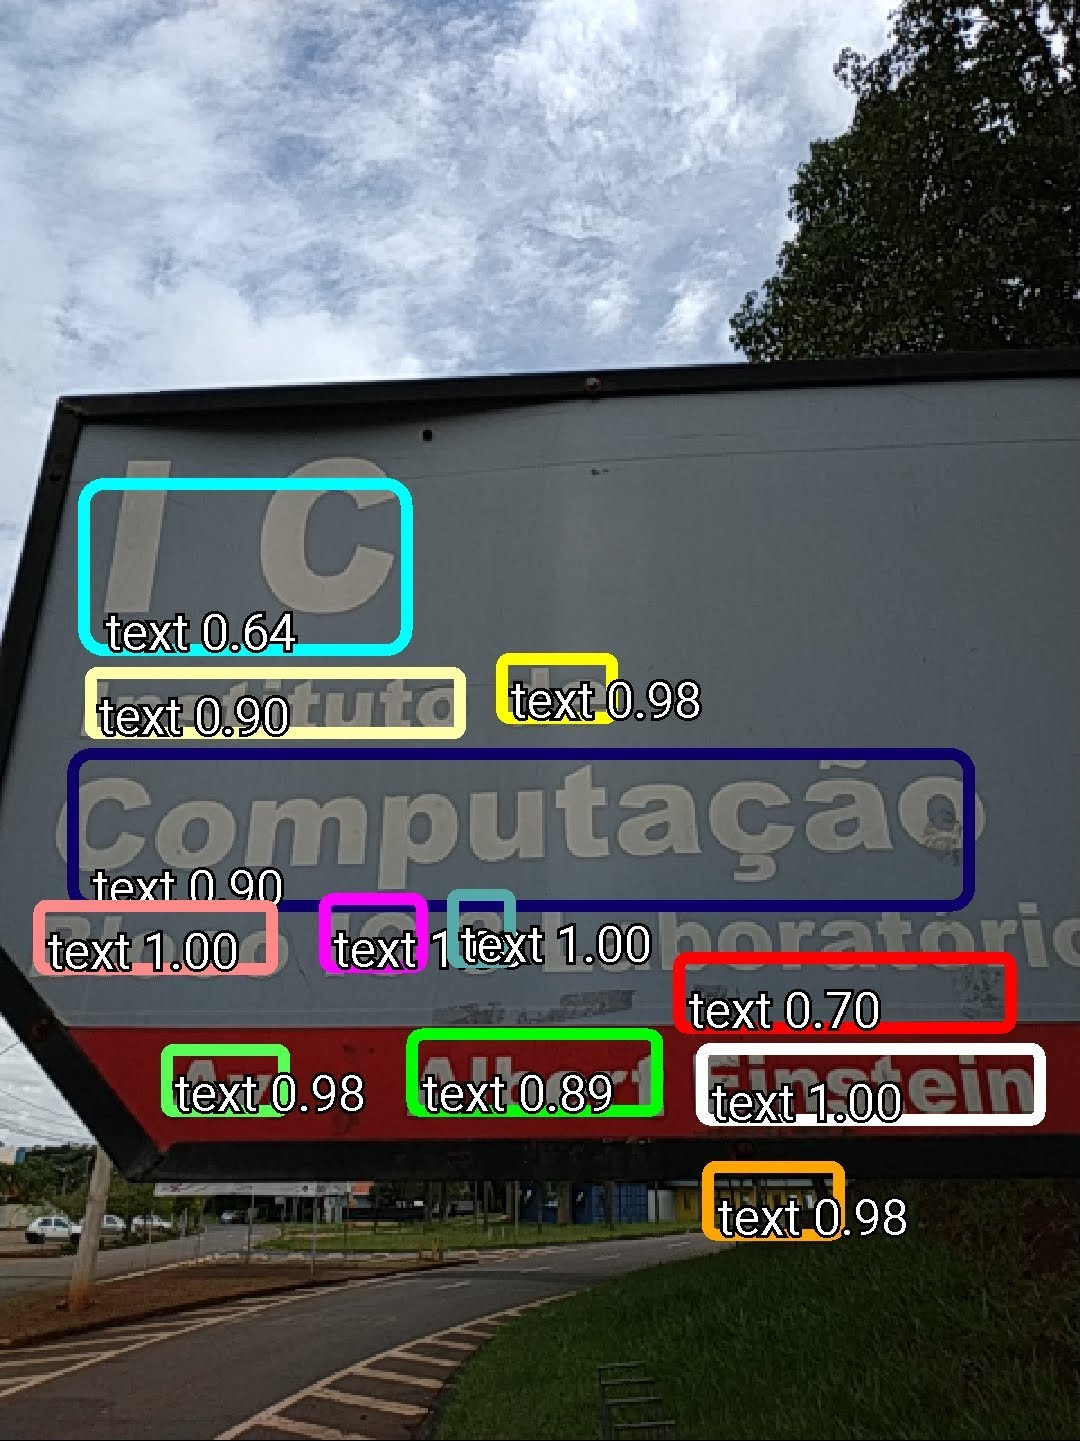
\includegraphics[width=0.49\textwidth]{Mobile/images/app26.jpg}


\caption{Example of scene text images captured with different zoom levels.}
\label{fig:ic-zoom}
\end{figure}
%%%%%%%%%%%%%%%%%
In Figure~\ref{fig:ic-zoom}, the effects of the size of the text on scene text images is shown. Images with smaller text (top left) are more difficult to detect, while image with medium to big text are easier and have better results, as shown in Figure~\ref{fig:sample_good}. 



\begin{figure}[h!]
\centering
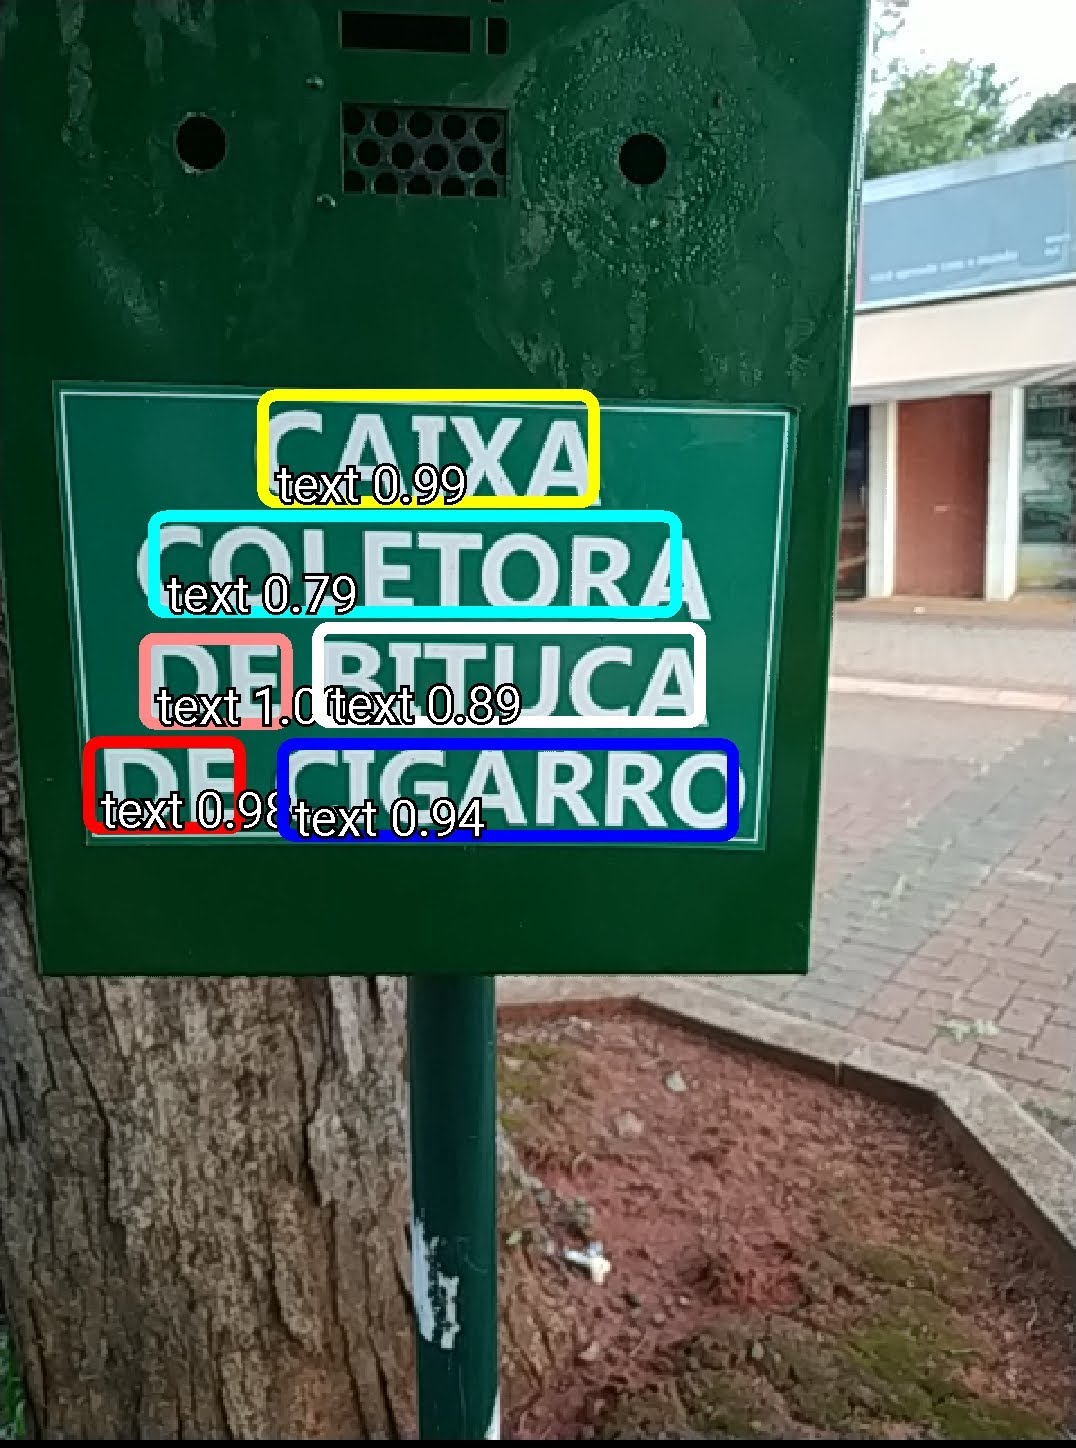
\includegraphics[width=0.49\textwidth]{Mobile/images/app03.jpg}
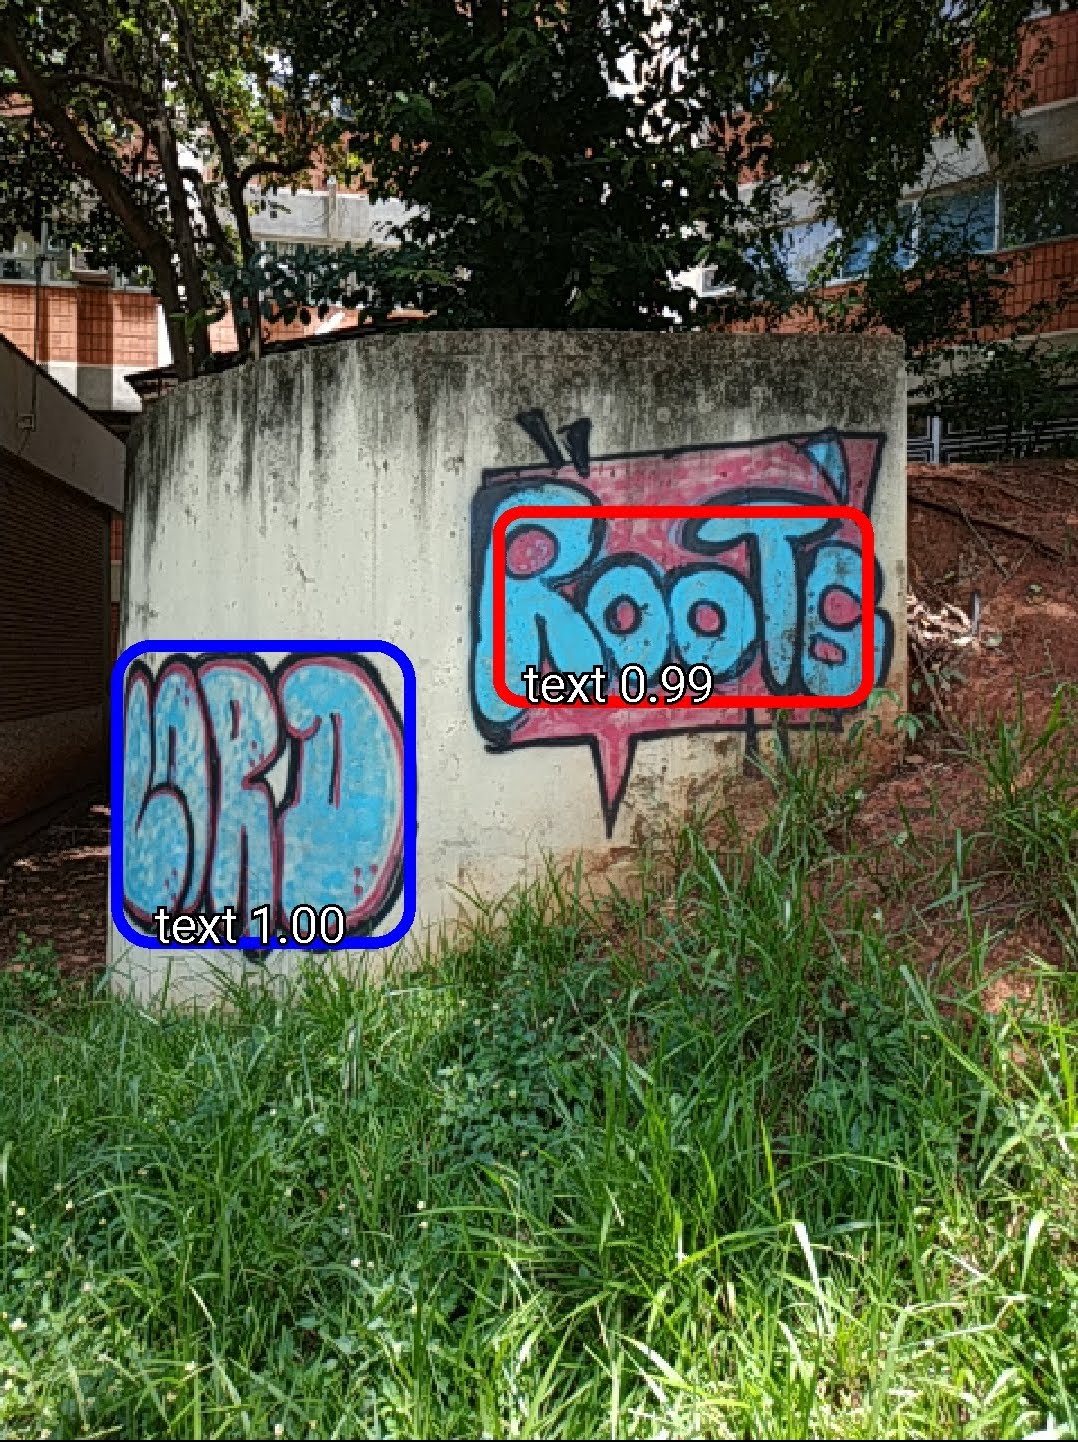
\includegraphics[width=0.49\textwidth]{Mobile/images/app09.jpg}

\vspace{1.5mm}

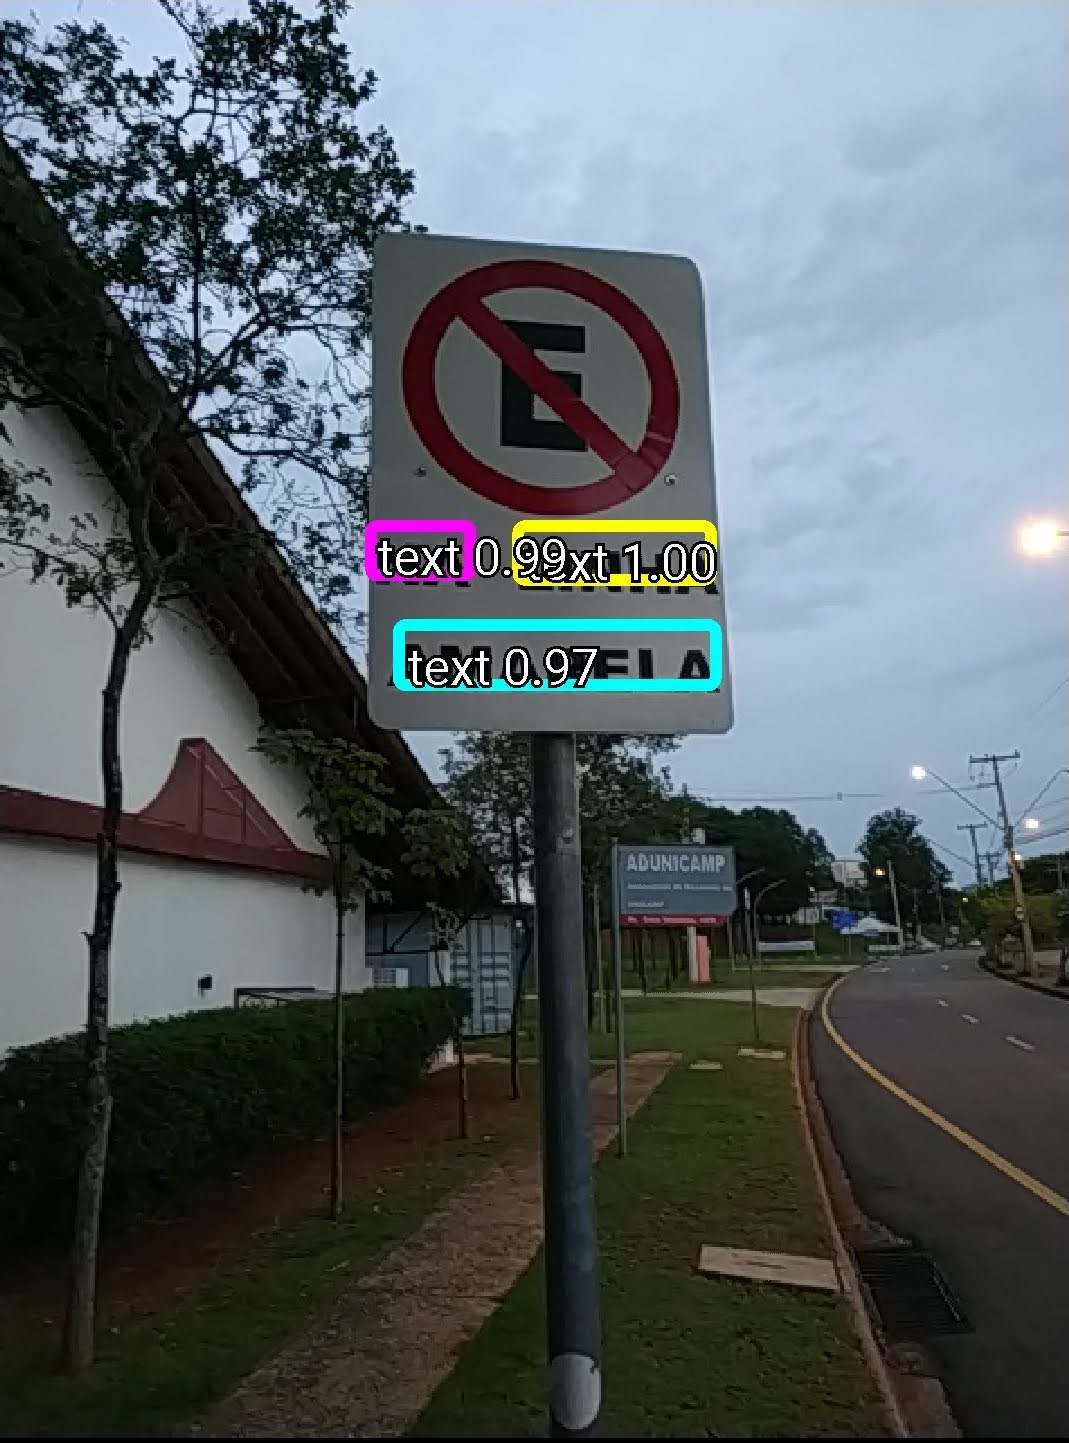
\includegraphics[width=0.49\textwidth]{Mobile/images/app07.jpg}
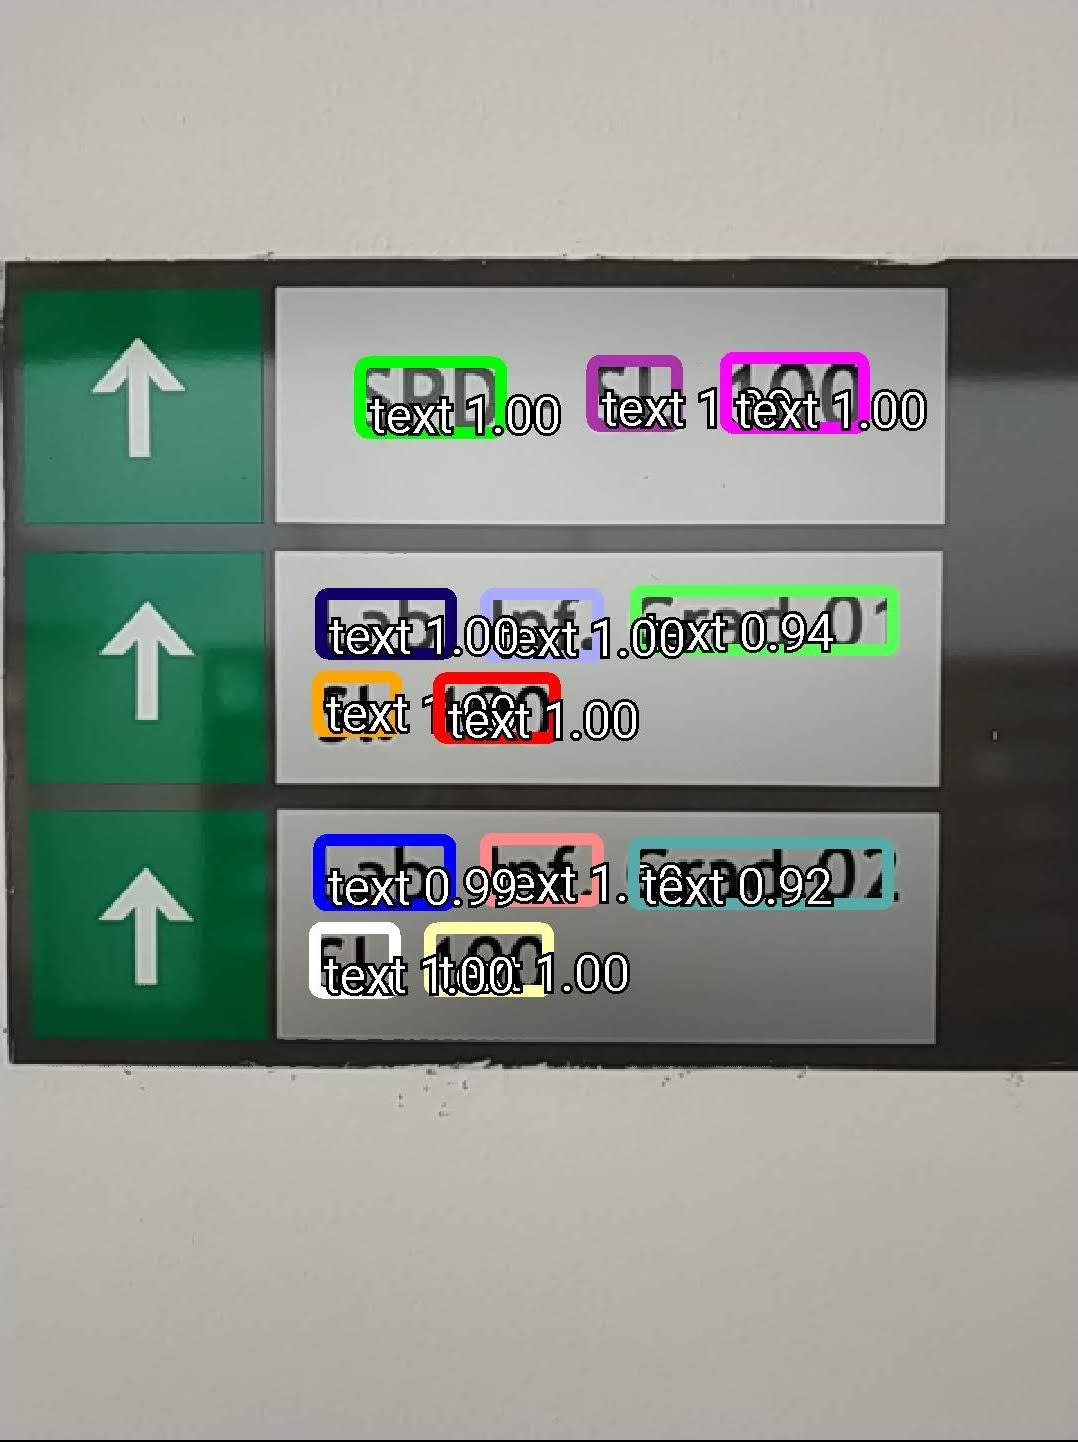
\includegraphics[width=0.49\textwidth]{Mobile/images/app11.jpg}


\caption{Example of scene text images with good results on our application.}
\label{fig:sample_good}
\end{figure}
%%%%%%%%%%%%%%%%%

Even though the system was not trained with handwritten text, the results of text detection on handwritten text, such as in Figure~\ref{fig:handwritten}, are very promising. Good detection results were obtained on handwritten text on a complex background (top left) and even on multilingual text (bottom left). 
\begin{figure}[h!]
\centering
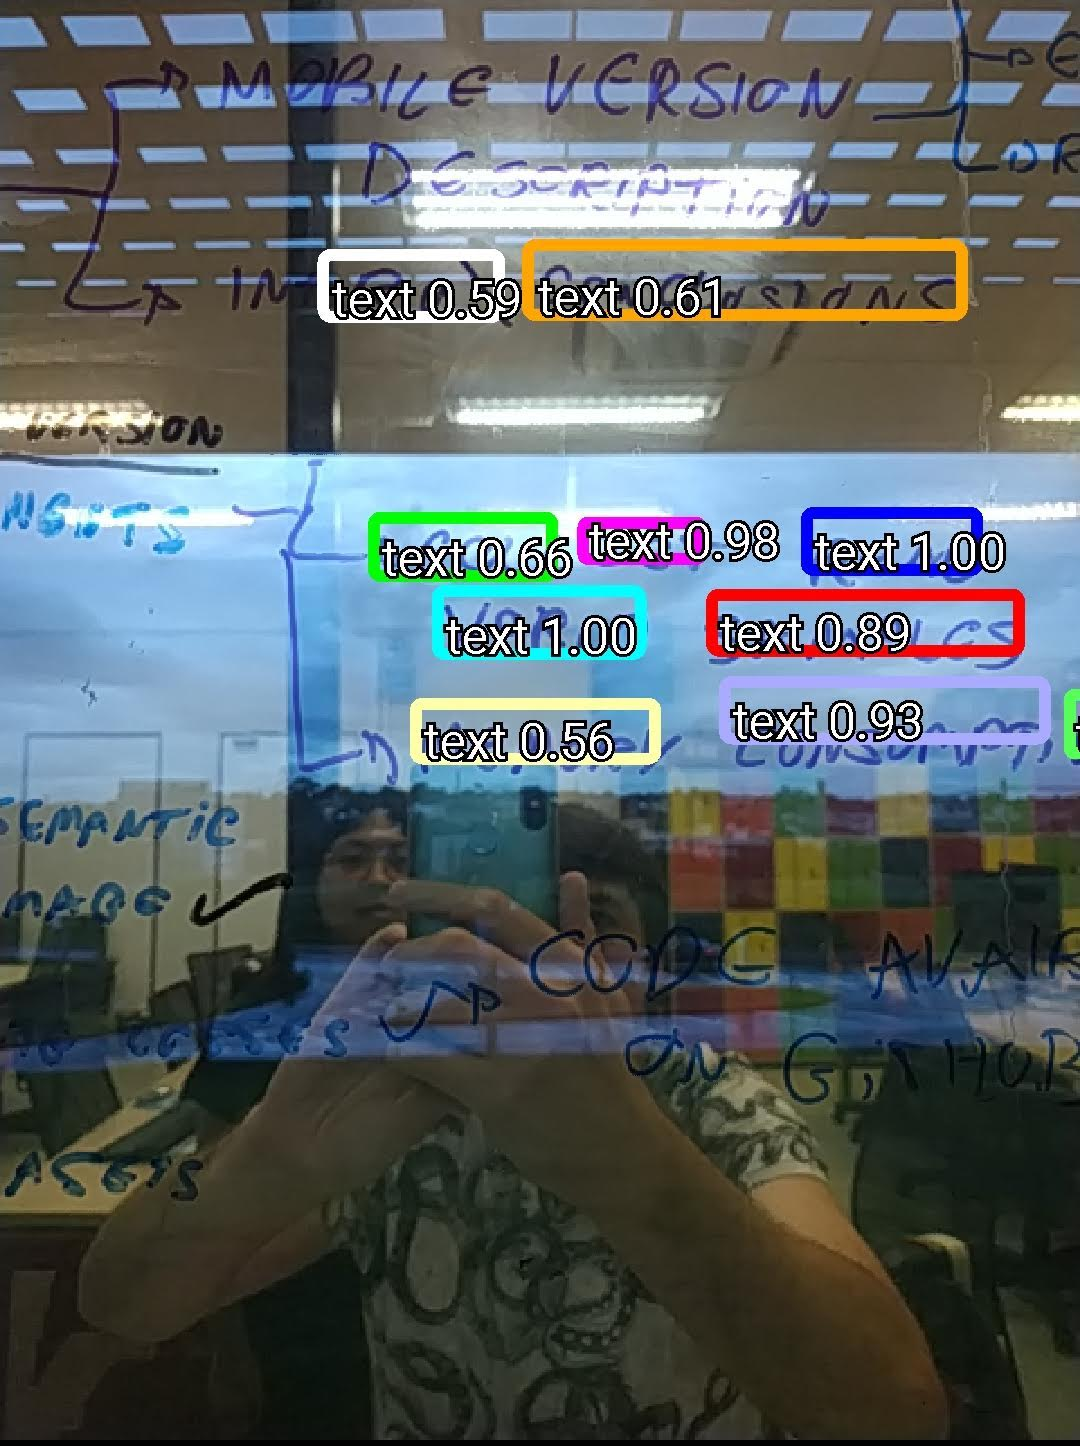
\includegraphics[width=0.49\textwidth]{Mobile/images/app22.jpg}
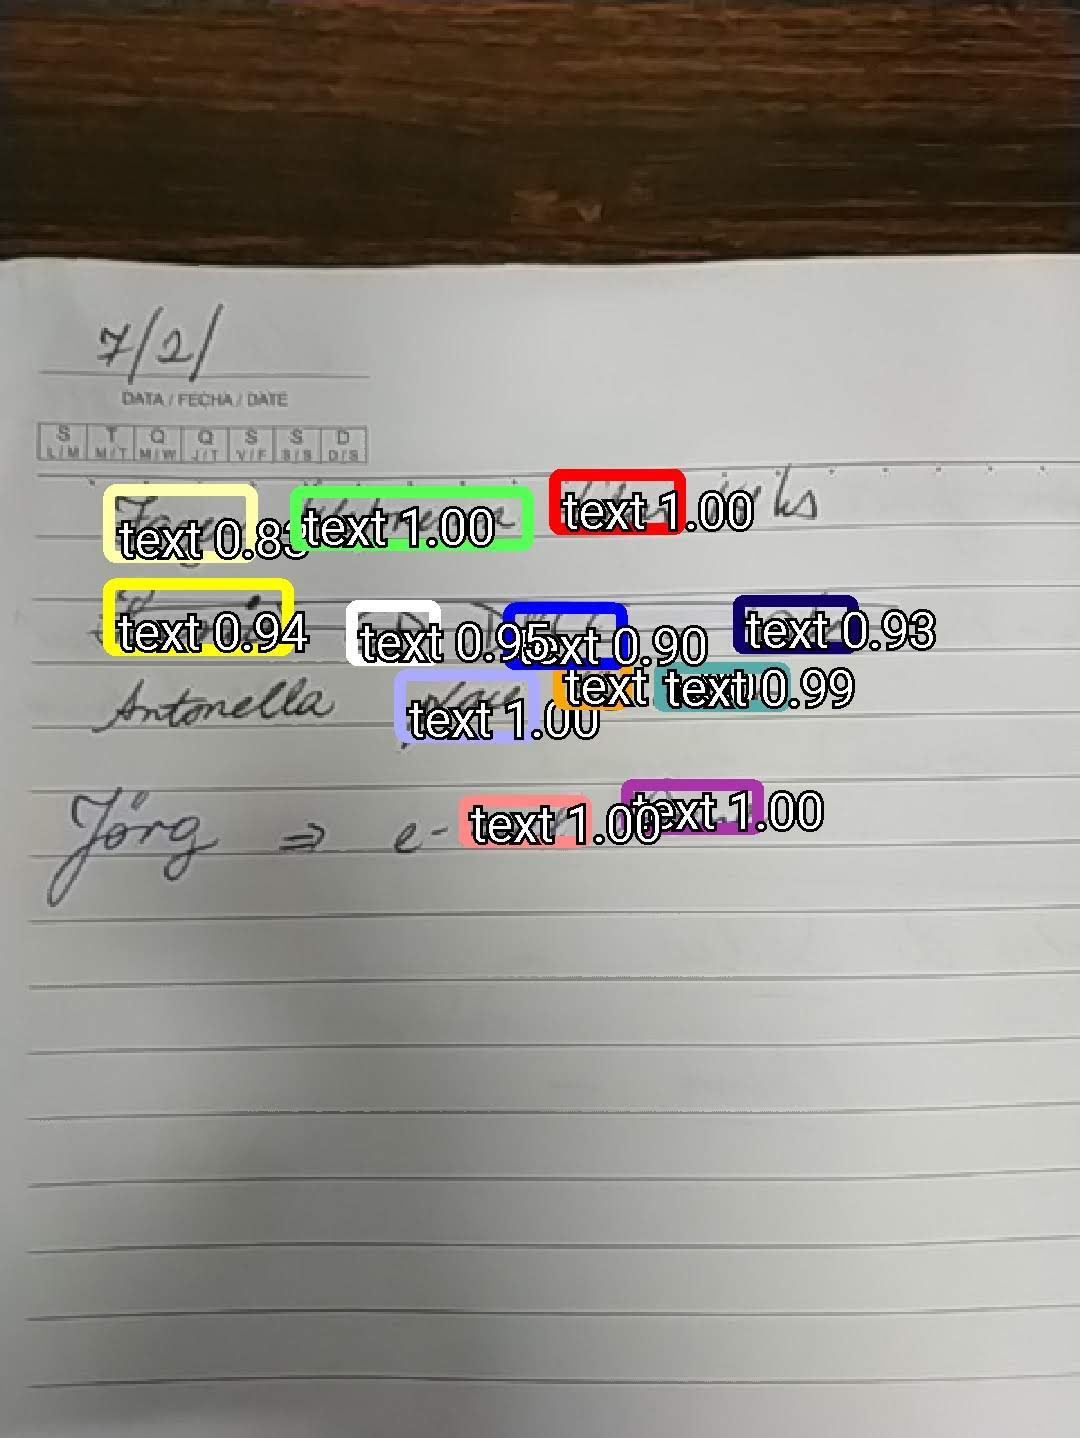
\includegraphics[width=0.49\textwidth]{Mobile/images/app31.jpg}

\vspace{1.5mm}

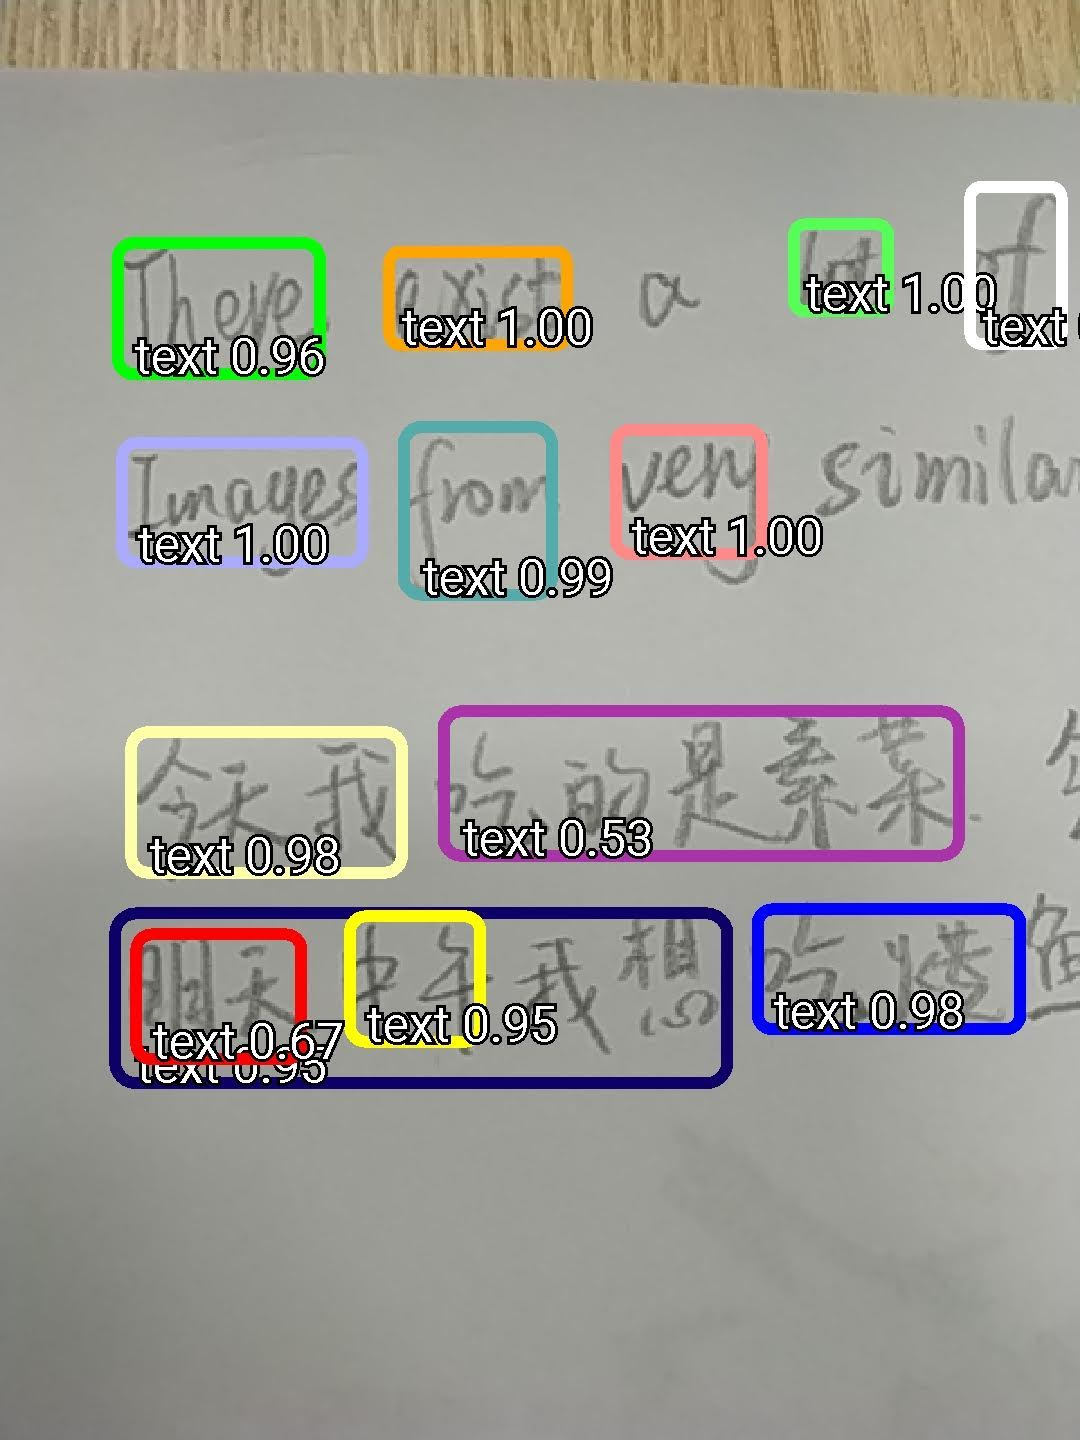
\includegraphics[width=0.49\textwidth]{Mobile/images/app17.jpg}
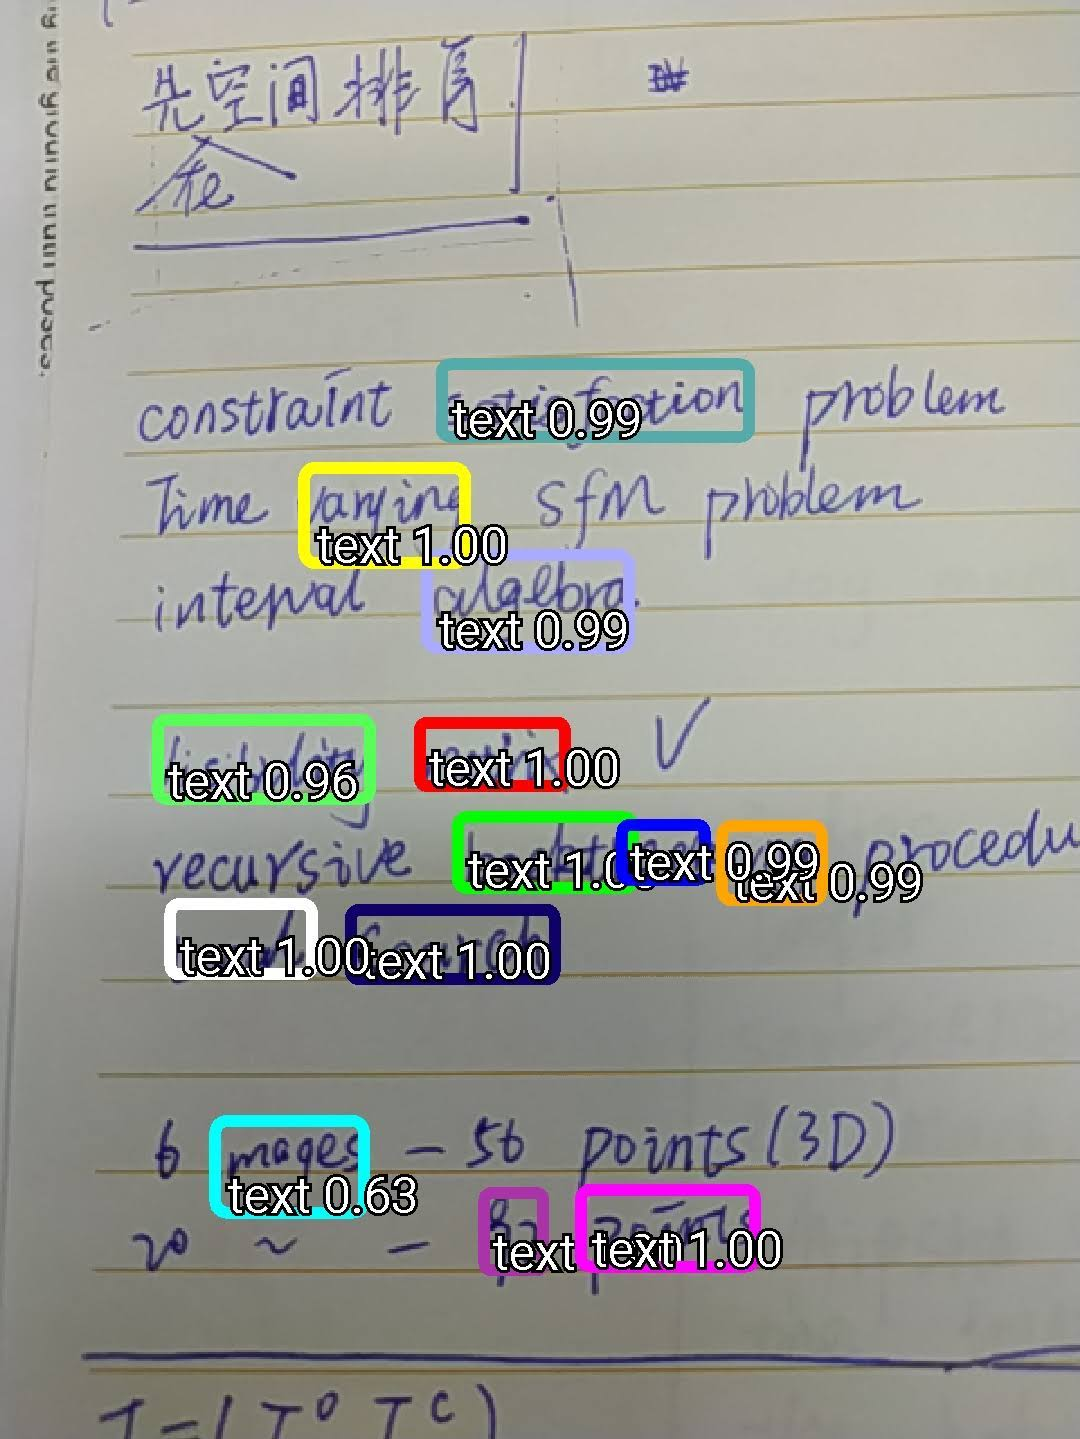
\includegraphics[width=0.49\textwidth]{Mobile/images/app18.jpg}


\caption{Example of handwritten text, with complex backgrounds and multilingual text.}
\label{fig:handwritten}
\end{figure}

%\begin{figure}[!t]
%	\centering
%	\hspace{0.1mm}
%	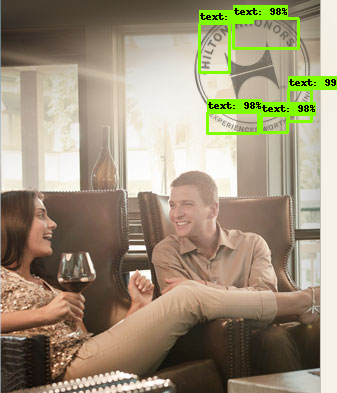
\includegraphics[height=0.27\columnwidth]{ICIP_frankenstein/figs/qualitative-results/icdar11-success-69.png}
%	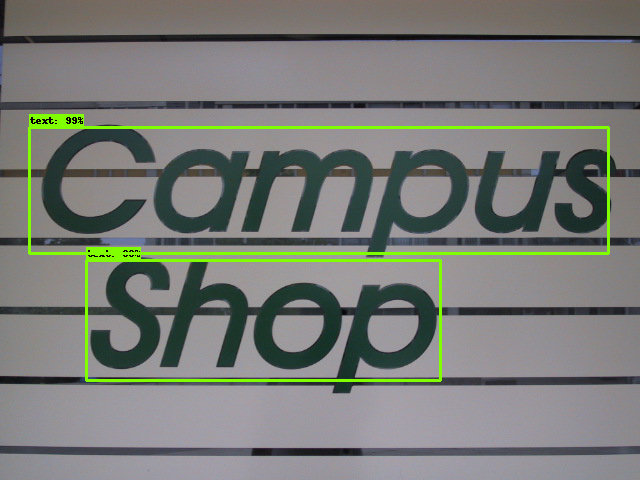
\includegraphics[height=0.27\columnwidth]{ICIP_frankenstein/figs/qualitative-results/icdar13-success-5.png}
%    \\ \vspace{0.5mm}
%	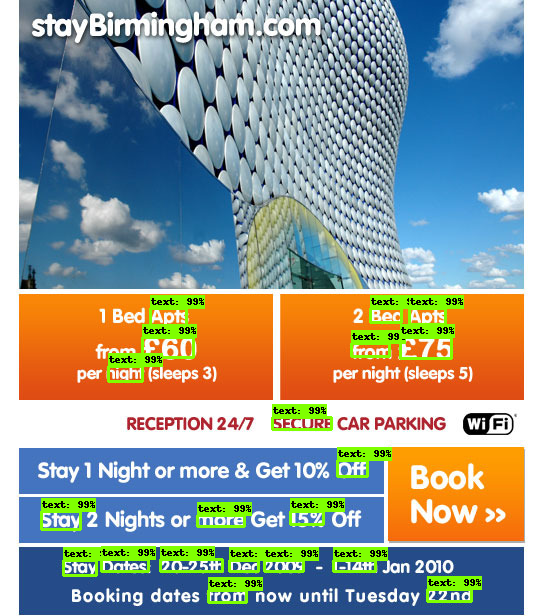
\includegraphics[height=0.27\columnwidth]{ICIP_frankenstein/figs/qualitative-results/icdar11-failure-10.png}
%	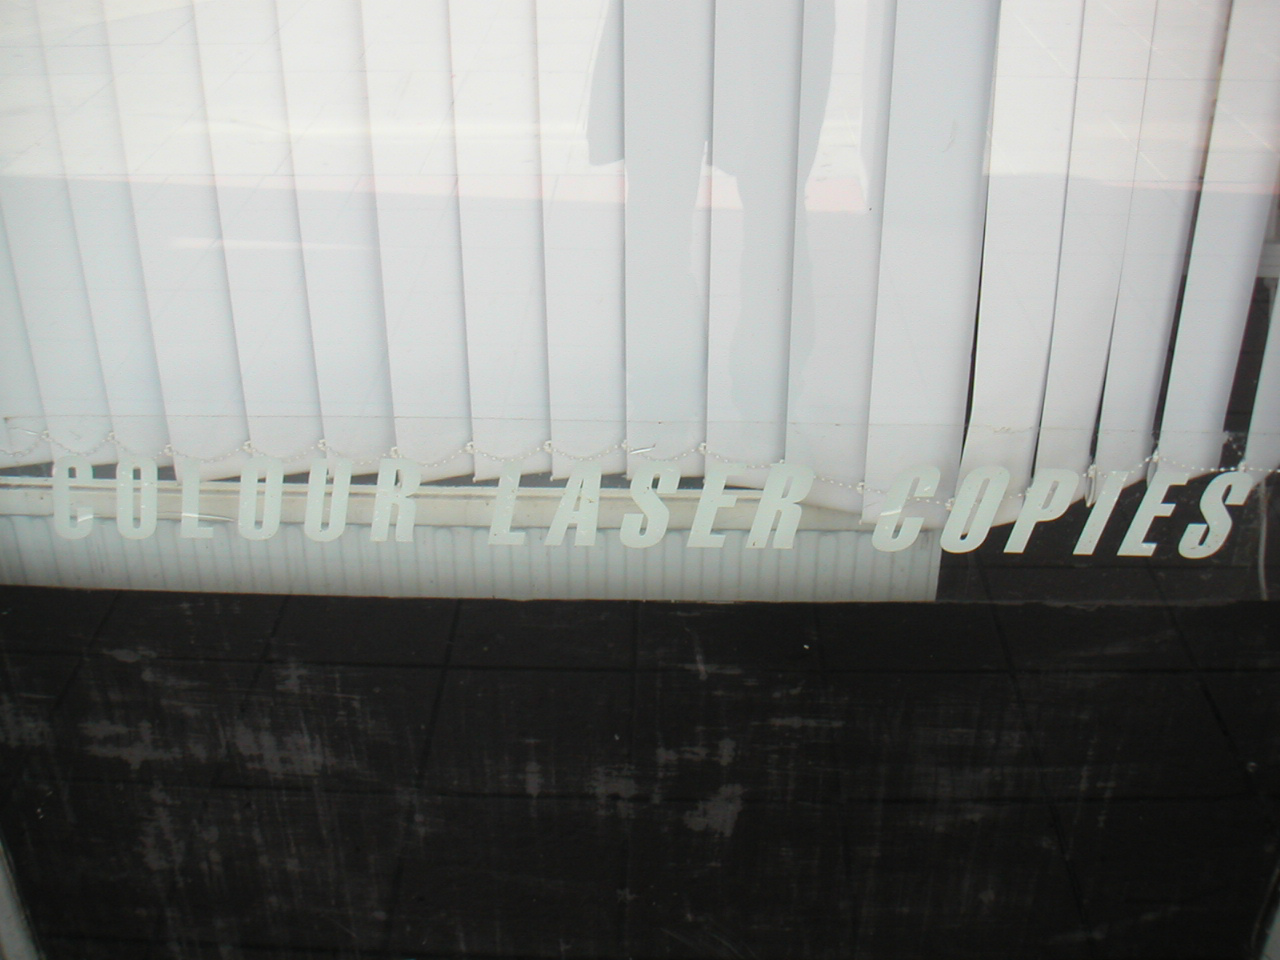
\includegraphics[height=0.27\columnwidth]{ICIP_frankenstein/figs/qualitative-results/icdar13-failure-185.png}
%	\caption{Examples of success (first line) and failure (second line) cases of the proposed approach for the ICDAR'11 (first column) and ICDAR'13 (second column) datasets.}
%	\label{fig:qualitative-results}
%\end{figure}



% Regarding the efficiency, in terms of processing time, the proposed method presented a very competitive results, taking only $0.09$ seconds per image, on average. This obtained processing time meets the results presented by the authors, which reported a computing speed about $0.02$ seconds per frame, considering an input image of $1,242 \times 375$ pixels.  For the disk usage performance, the lighter deep learning-based model was produced by SqueezeDet, with a size of $23.10$MB. On the other hand, the heaviest deep learning-based model was produced by SSTD network, with a size of $248.20$MB.
%
%\todo[inline]{Include the values for YOLOv3 in the table below}
%
% \begin{table}[!t]
%     \centering
%     \caption{Processing time per image, in seconds, for the evaluated deep learning-based methods.}
%     \label{tab:comparison-efficiency-time-proc-deep-methods-icdar11-icdar13}
%     \resizebox{\columnwidth}{!}{ 
%     \begin{tabular}{lrrr}
%         \topline
%         \headcol
%         \headcol \textbf{Methods} & \textbf{ICDAR'11} & \textbf{ICDAR'13} & \textbf{Average} \\
%         \midline
%         SSTD                      & $0.45$               & $0.55$               & $0.50$              \\ \hline
%         TextBoxes                 & $0.45$               & $0.53$               & $0.49$              \\ \hline
%         TextBoxes++               & $1.70$               & $1.87$               & $1.79$              \\ \hline
%         MobText           & $5.62$               & $4.32$               & $4.97$              \\ \hline
%         % YOLOv3                    & $6.84$               & $7.42$               & $7.13$              \\ \hline
%         % SqueezeDet                & $0.08$               & $0.09$               & $0.09$              \\
%       \bottomlinec
%     \end{tabular}}
% \end{table}
% %		
% \begin{table}[!t]
%     \centering
%     \caption{Comparison of efficiency, in terms of disk usage, among the evaluated deep learning-based methods.}
%     \label{tab:comparison-efficiency-disk-usage-deep-methods}
%     \begin{tabular}{lr}
%         \topline
%         \headcol \textbf{Methods} & \textbf{Disk usage (MB)}    \\
%         \midline
%         SSTD                      & $248.20$                    \\ \hline
%         TextBoxes                 & $95.10$                     \\ \hline
%         TextBoxes++               & $139.10$                    \\ \hline
%         MobText           & $37.00$                     \\ \hline
%         % YOLOv3                    & $246.30$                    \\ \hline
%         % SqueezeDet                & $23.10$                     \\
%       \bottomlinec
%     \end{tabular}
% \end{table}

%    \section{Discussion}
\label{sec:discussion}

The experimental results presented in Section~\ref{sec:results}  provided to us an overview of the performance results of evaluated methods, in terms of their effectiveness and efficiency, which are discussed in this section.

Figures~\ref{fig:non-deep-methods-efficacy-and-efficiency} and~\ref{fig:deep-methods-efficacy-and-efficiency} summarize, for non-deep and deep methods, respectively, the obtained results considering the metrics used to evaluate the effectiveness of the evaluated methods (i.e., Precision, Recall, and F-measure), along with
the metrics for measuring the efficiency of these methods, considering the ICDAR'11 and ICDAR'13 datasets. 

As we can observe in Figure~\ref{fig:non-deep-methods-efficacy-and-efficiency}, the SnoopText method presented several limitations in terms of efficiency,  although it has achieved very competitive results in terms of effectiveness.  When we take a look at the SnoopText's implementations, we can see that several improvements can be done towards minimizing the computer resources required for this method. For instance, the authors saved the pre-trained models without using any data compression. Also, the re-implementation of this method considering a faster programming language (C/C++) can potentially improve considerably the time consumption.

The Scene Text Recognition method also achieved very competitive results for the ICDAR'11 dataset, as well as impressive results concerning the processing time and disk usage, in both datasets. However, the major limitation of this method concerns the low precision achieved in the experimental results, from which we glimpse some further investigation such as the use of moderns visual descriptors in replacement of descriptors proposed in the original paper. In fact, the Canny Text Detection presented competitive results by adopting the mean LBP to build a second-stage pruning classifier.

Regarding the deep learning-based methods, we also identify several limitations in terms of effectiveness and efficiency (Fig.~\ref{fig:deep-methods-efficacy-and-efficiency}). Firstly, the most accurate networks, in terms of precision and recall, obtained the lowest results in terms of processing time (SSD-MobileNetV2) or disk usage (SSTD). On the other hand, the SqueezeDet network was the most efficient network, which obtained a very impressive result considering the processing time and disk usage. But, at the same time, this network achieved poor results, in comparison with other networks, mainly in terms of its precision. These findings suggest  that further investigation is needed towards improving the efficiency of the most accurate networks.

Finally, different from to what was pointed out by~\cite{Ye2015PAMI}, experimental results with deep learning architectures proposed for object detection problems (e.g., MobilenetV2 and YOLOv3) suggest that adapting those networks for text detection is a promising research venue. Along with these networks, the TextBoxes++ presented a good balance between effectiveness and efficiency and also it seems to be a promising method for further investigation.

% The performed comparative study allows us to point out the following considerations:
% \begin{enumerate}
%     \item Different from to what was pointed out by~\cite{Ye2015PAMI}, experimental results with deep learning architectures proposed for object detection problems (e.g., MobilenetV2 and YOLOv3) suggest that adapting those networks for text detection is a promising research venue.
% \end{enumerate}
%
\begin{figure}[H]
    \centering
    \begin{subfigure}[t]{0.98\textwidth}
        \centering
        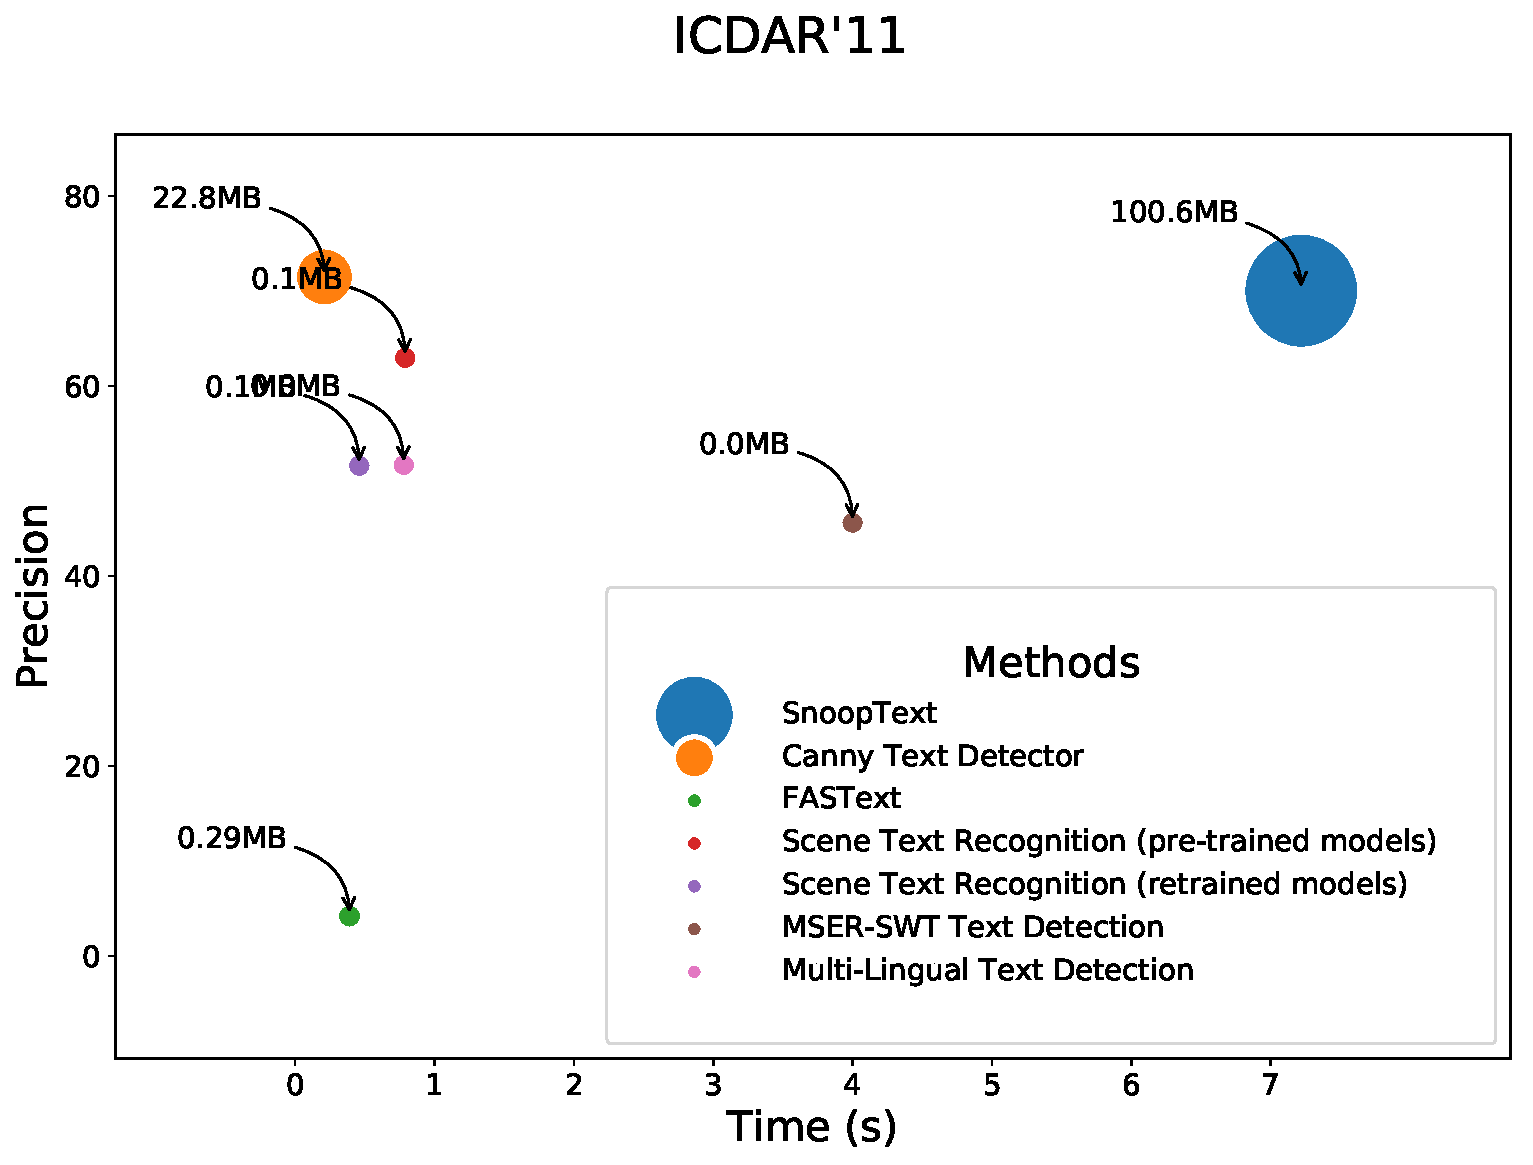
\includegraphics[height=0.25\textheight]{figs/efficacy-and-efficiency/non-deep-methods-icdar11-precision.pdf}
        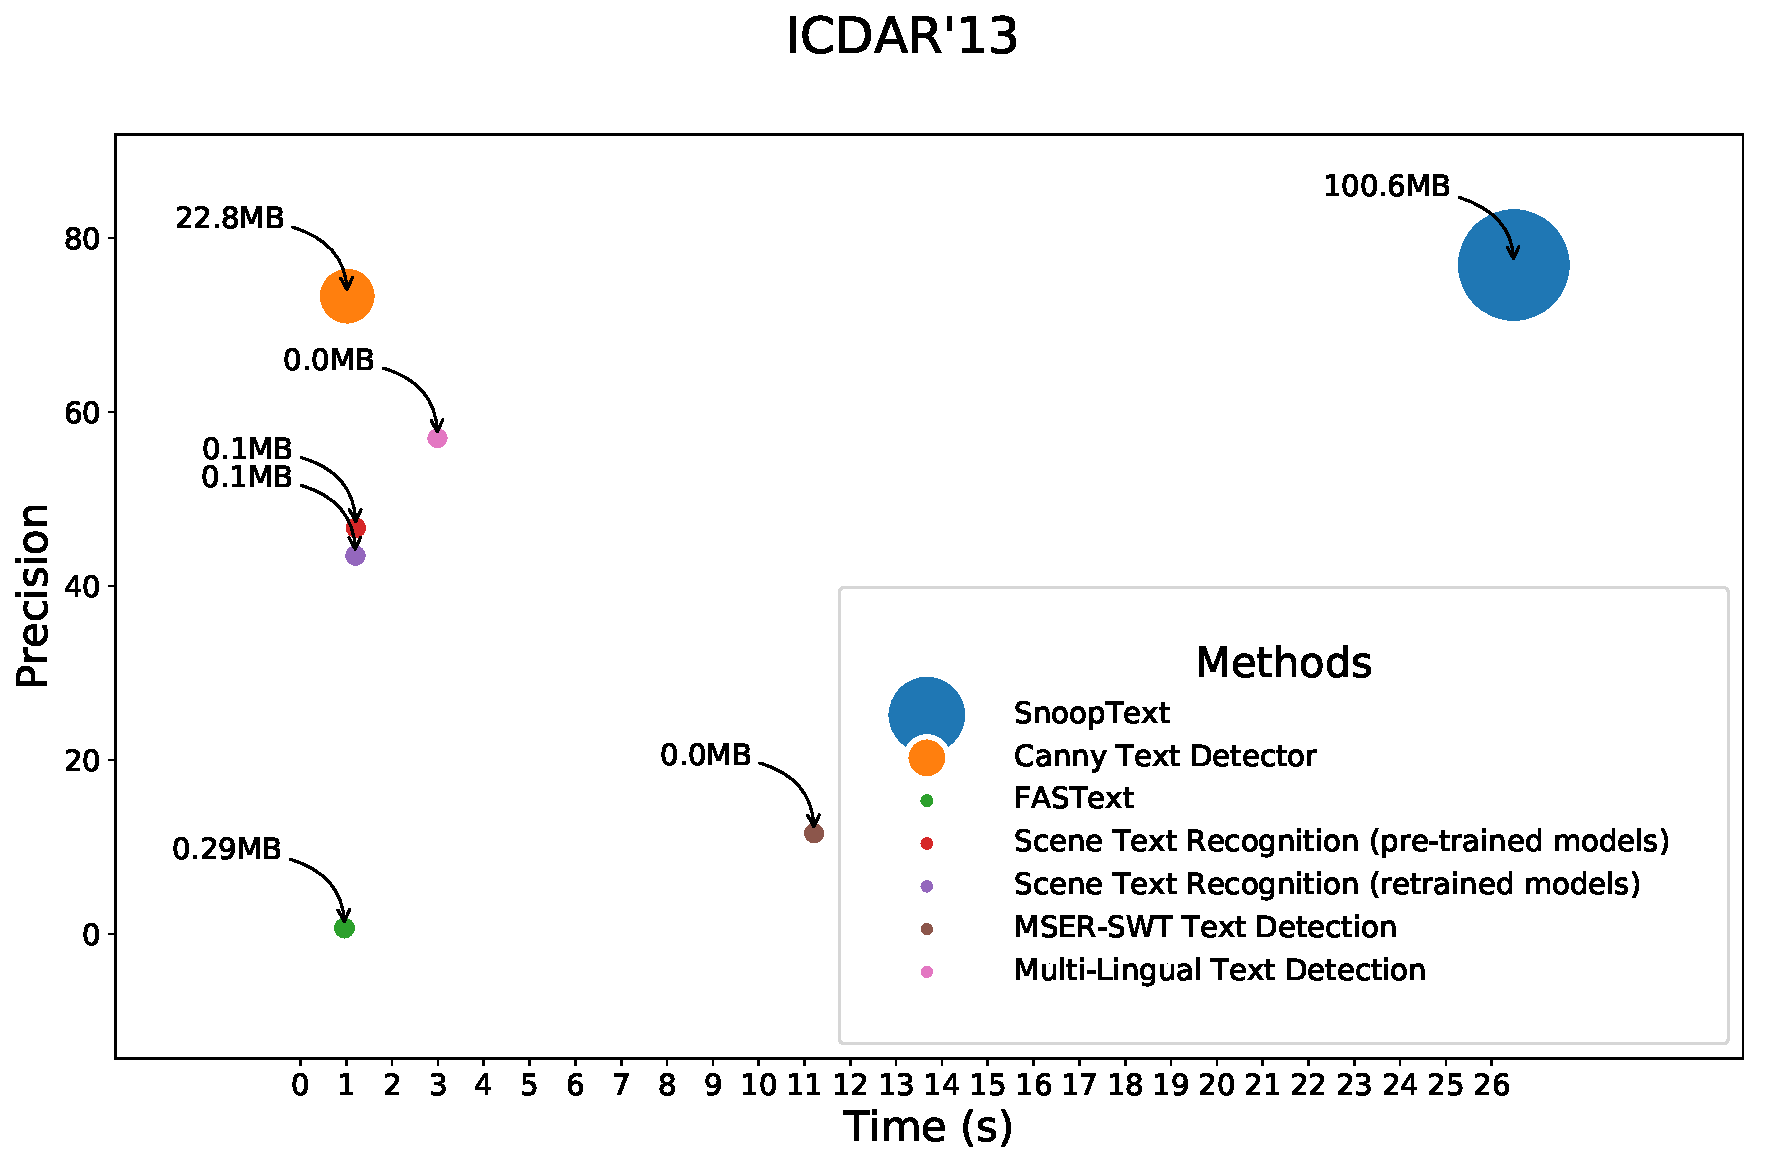
\includegraphics[height=0.25\textheight]{figs/efficacy-and-efficiency/non-deep-methods-icdar13-precision.pdf} \\
        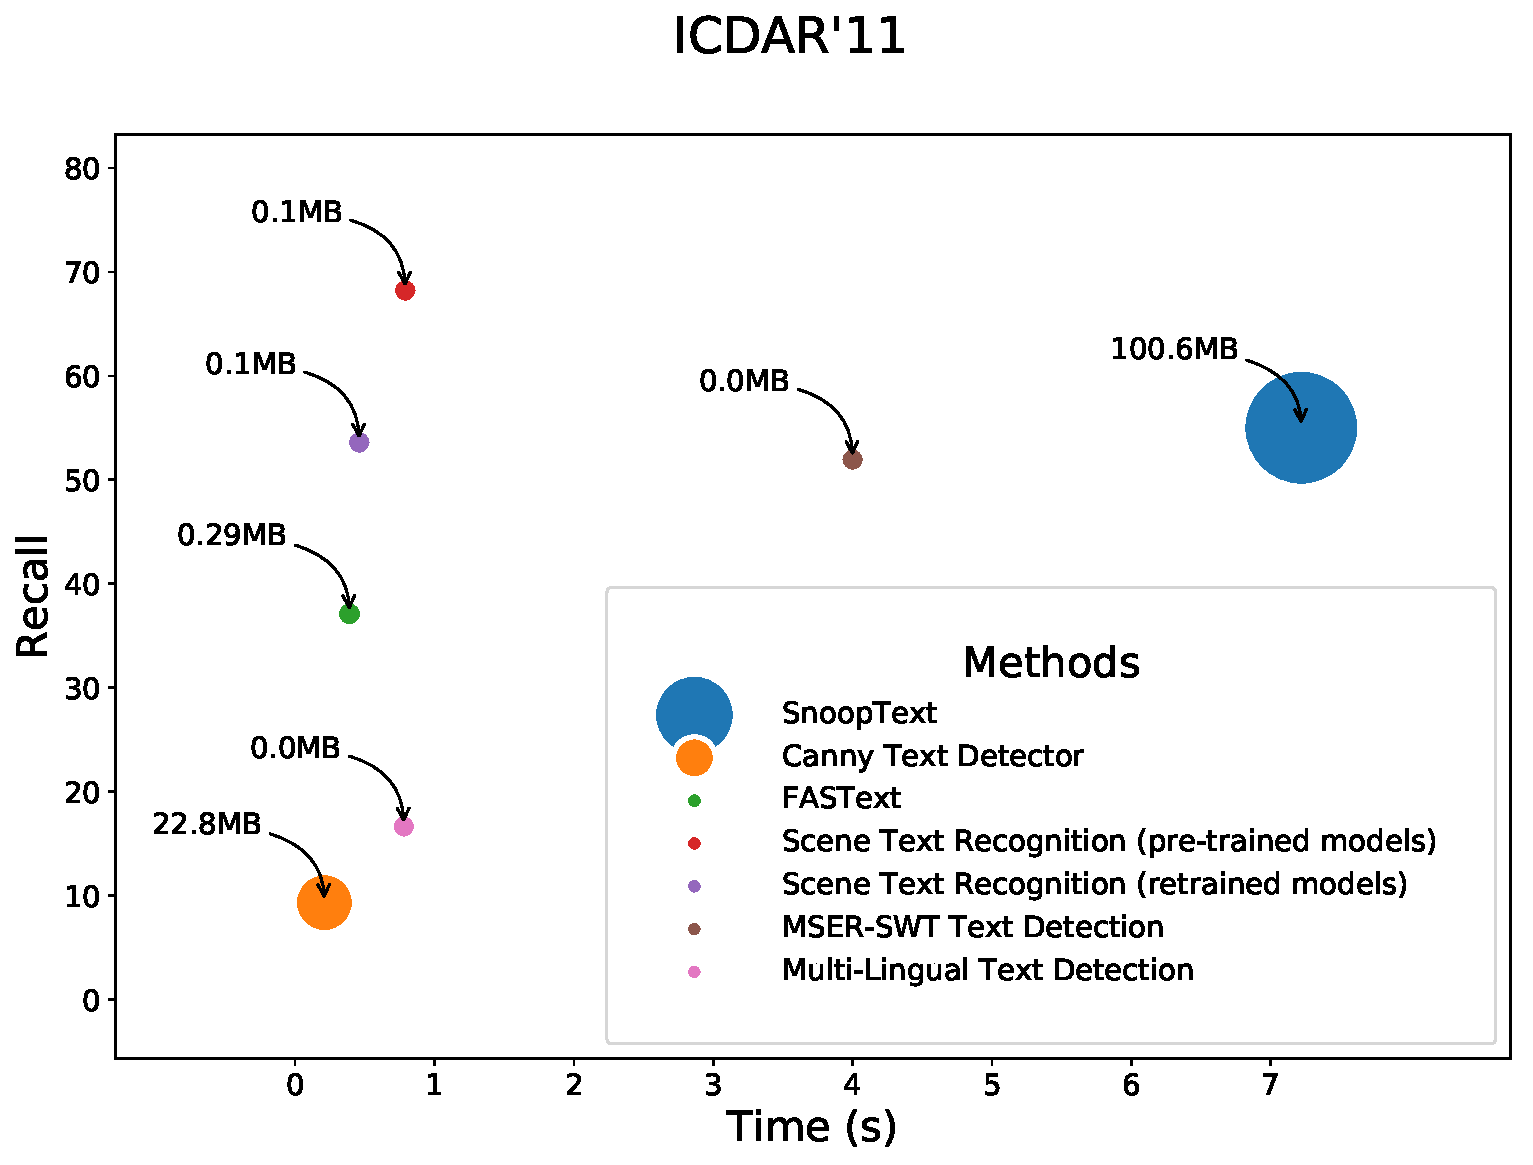
\includegraphics[height=0.25\textheight]{figs/efficacy-and-efficiency/non-deep-methods-icdar11-recall.pdf}
        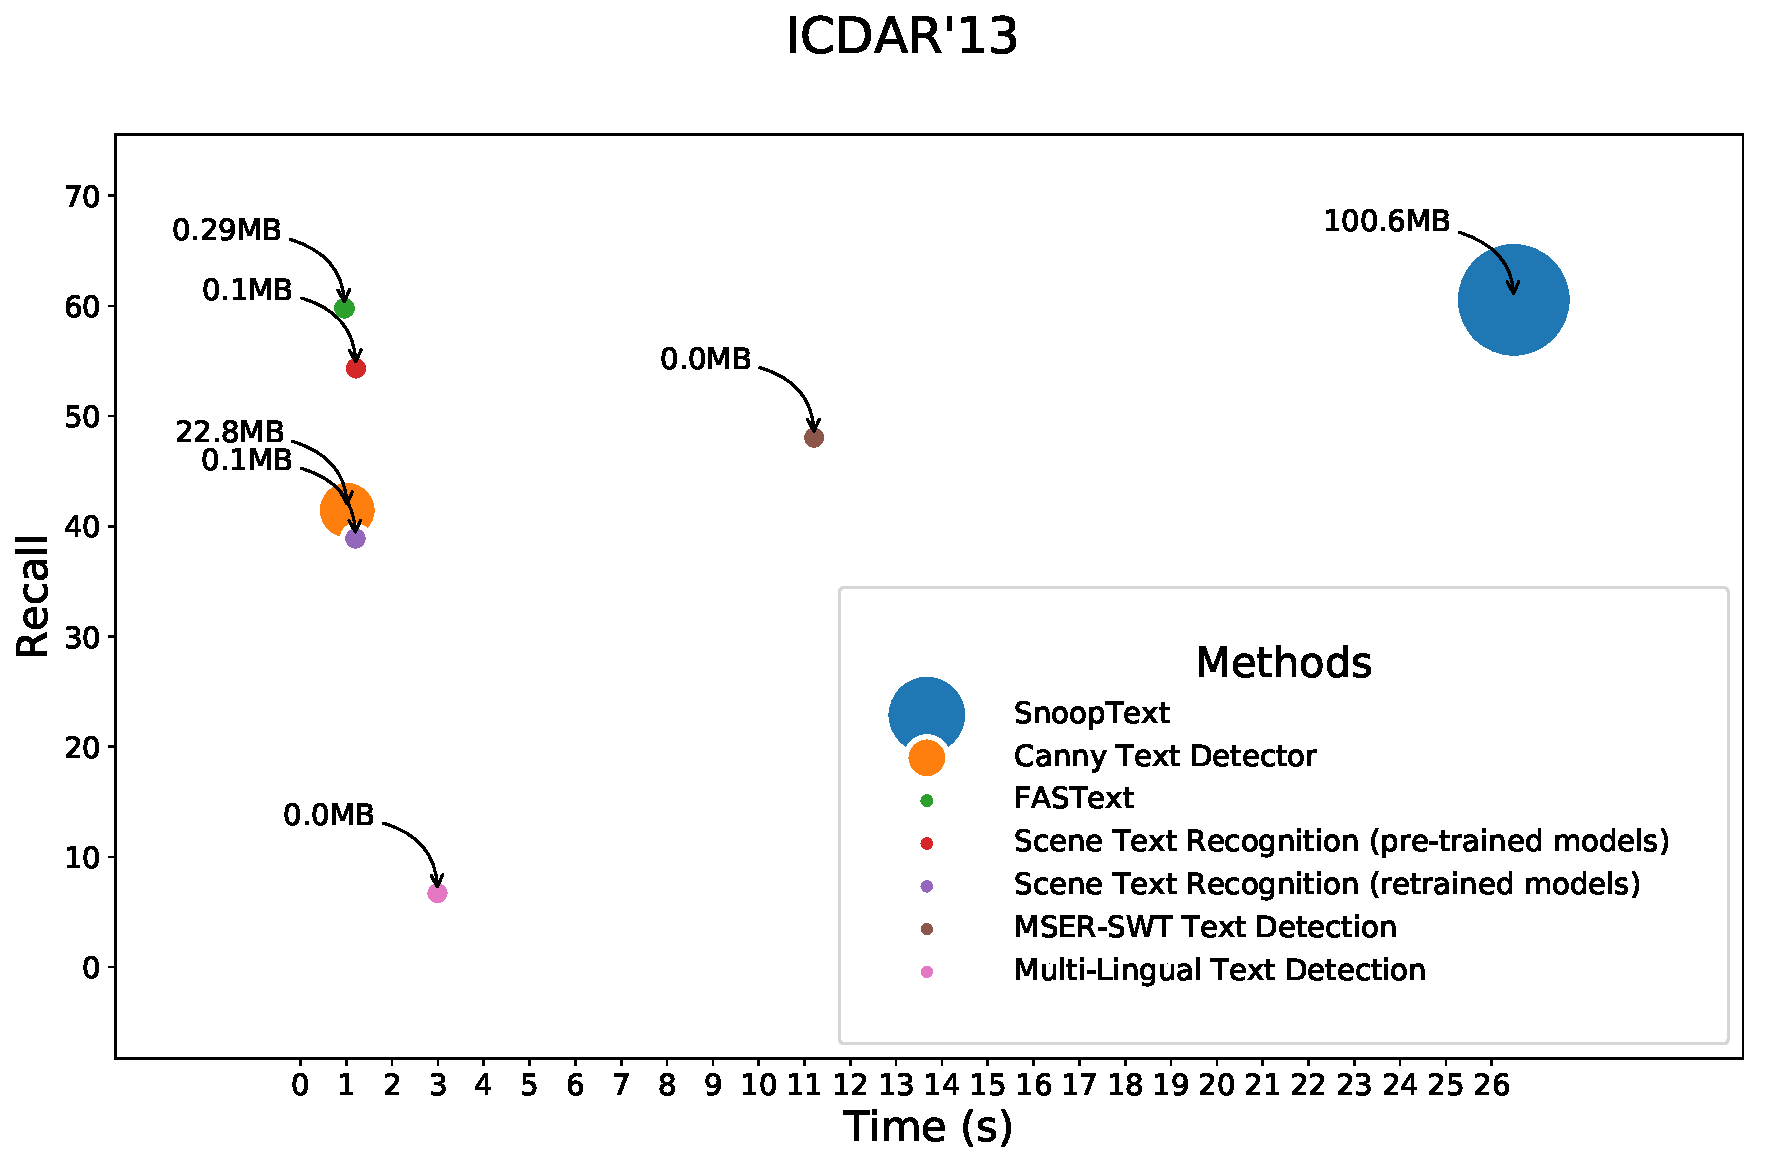
\includegraphics[height=0.25\textheight]{figs/efficacy-and-efficiency/non-deep-methods-icdar13-recall.pdf} \\
        \includegraphics[height=0.25\textheight]{figs/efficacy-and-efficiency/non-deep-methods-icdar11-f-measure.pdf}
        \includegraphics[height=0.25\textheight]{figs/efficacy-and-efficiency/non-deep-methods-icdar13-f-measure.pdf}
    \end{subfigure}
    \caption{Comparison results among the non-deep-based methods considering aspects of efficacy and efficiency.}
    \label{fig:non-deep-methods-efficacy-and-efficiency}
\end{figure}
%
\begin{figure}[H]
    \centering
    \begin{subfigure}[t]{0.98\textwidth}
        \centering
        \includegraphics[height=0.25\textheight]{figs/efficacy-and-efficiency/deep-methods-icdar11-precision.pdf}
        \includegraphics[height=0.25\textheight]{figs/efficacy-and-efficiency/deep-methods-icdar13-precision.pdf} \\
        \includegraphics[height=0.25\textheight]{figs/efficacy-and-efficiency/deep-methods-icdar11-recall.pdf}
        \includegraphics[height=0.25\textheight]{figs/efficacy-and-efficiency/deep-methods-icdar13-recall.pdf} \\
        \includegraphics[height=0.25\textheight]{figs/efficacy-and-efficiency/deep-methods-icdar11-f-measure.pdf}
        \includegraphics[height=0.25\textheight]{figs/efficacy-and-efficiency/deep-methods-icdar13-f-measure.pdf}
    \end{subfigure}
    \caption{Comparison results among the deep-learning-based methods considering aspects of efficacy and efficiency.}
    \label{fig:deep-methods-efficacy-and-efficiency}
\end{figure}



%    \section{Conclusions}
\label{sec:conclusions}

This report refers to the second deliverable related to the project Multi-Lingual Text Spotting and Recognition (MLTSR). The report describes performed experiments aiming to evaluate text detection solutions. Two types of approaches were considered: methods that do not rely on deep learning strategies; and methods that take advantage of deep-learning-based architectures. Those methods were evaluated in terms of effectiveness and efficiency. The effectiveness evaluation considered the capacity of the method in properly locating texts within images; while efficiency aspects were evaluated in terms of processing time, and storage requirements. Performed experiments considered widely used benchmarks (evaluation metrics and datasets). 

As expected, the deep-learning-based methods presented top-performance results in terms of effectiveness, while the non-deep methods showed to be very efficient options for text detection. However, we noticed some exceptions to which we could pay attention in our future investigations. In opposite directions, we found some efficient deep learning methods (SqueezeDet, SSD-MobilenetV2, and TextBoxes), and effective non-deep methods (SnoopText, Scene Text Recognition methods, and Canny Text Detection). Further investigation to find the mechanisms responsible for these unexpected results might be a good source of inspiration towards achieving fast and accurate models for text detection in constrained processing scenarios.

The conducted comparative study provides insights about traditional and recently proposed approaches for the text detection problem, opening promising research directions for the MSTSR project.
Achieved results suggest that some of the evaluated methods are good candidates to be further improved, in terms of both efficiency and effectiveness, in future work. The goal is to have proper methods for prototyping and deploying in restrictive computing devices. 
Some of those research venues include:

%\todo[inline]{Revise the list of possible research venues below.}

\begin{enumerate}

    \item Extend the evaluation protocol to consider:
    \begin{itemize}
        \item Other datasets, such as those related to Focused Scene Text (2013-2015) -- Word Recognition, and End to End; Incidental Scene Text (2015) -- Word Recognition, and End to End; and MLT (2017) -- Text Detection, Word Identification, and both;
        \item Evaluation protocols suitable for the evaluation of methods targeting end-to-end recognition scenarios.\footnote{Experiments involving those datasets and considering the most promising non-deep and deep solutions will be described in Deliverable E6.}
    \end{itemize}

    \item Improve the efficiency and effectiveness of the SnoopText method: SnoopText yielded competitive effectiveness results for both ICDAR'11 and ICDAR'13 datasets. We believe that its effectiveness may be further improved by investigating deeply the impact of its parameter setting. Regarding efficiency, one alternative would be to re-implement (some of) its components in another, possibly, faster language.
    
    \item Use other descriptors, such as LPQ, HOG, LBP, and M-LBP to train the classifiers (first and second ones) of the Scene text detection implementation proposed by Neumann and Matas~\cite{Neumann2012CVPR}\cite{Neumann2016TPAMI}. The classifiers of the Scene text detection implementation use only binary descriptors to classify if a ER is a candidate character. However, a lot of research initiatives have been using texture descriptors because they are also very efficient to extract different discriminative features (see Fig.~\ref{fig:new_pipeline}).
    
    \item Improve the effectiveness of the FASText method by investigating other possibilities for the post-processing stage to detect multi-oriented bounding boxes.

    \item Investigate the use of the double thresholding strategy~\cite{Cho2016CVPR}, instead of using two classifiers, to extract candidate characters and remove false positives, as well as use tracking by hysteresis to increase the confidence of the characters classified as weak using OCR.
    %\todo[inline]{Add a reference for ``double thresholding''}
    
    \item Investigate other descriptors (e.g., LPQ and T-Hog) to build a pruning classifier for the Canny Text Detection method. Results of MSER and SWT are promising, but they demonstrated that suffer from a high rate of false positives. We will use a text/non-text classifier in order to eliminate false positives and observe the impact of this alternative in the final F-measure.
    
    \item Perform experiments for text detection using blocks of a Discrete Cosine Transform (DCT) along with grouping methods as geometric features (size of blocks, distance between blocks, etc.) given that some preliminary experiments showed promising results of DCT.
    
    \item Investigate the possibility of merging the best features of TextBoxes++ and SSD-MobilenetV2, i.e., take advantage of the adapted layers of TextBoxes++ to recognize oriented text along with the structure and final model size of SSD-MobilenetV2.
    
    \item Train an object-detection network like SSD-Mobilenetv2 to detect characters (a-Z,0-9) and use a grouping method to create word-level predictions. As we gonna have the value of each char, we can convert this to an end-to-end model.
\end{enumerate}
%
\begin{figure}[H]
    \centering
    \includegraphics[width=0.75\textwidth]{figs/new-pipeline-scene-text-recognition.pdf}
    \caption{Possible pipeline to be considered in further investigations to improve the Scene Text Recognition method.}
    \label{fig:new_pipeline}
\end{figure}

%    \appendices

\input{appendix_textboxesplusplus}
\input{appendix_ssd_mobilenetv2}
\input{appendix_descriptors_library}

    \section*{Acknowledgment}
We thank SRBR for the financial support.


    


   % \listoftodos
    
    % Can use something like this to put references on a page
    % by themselves when using endfloat and the captionsoff option.
    \ifCLASSOPTIONcaptionsoff
    \newpage
    \fi
    
    
    % trigger a \newpage just before the given reference
    % number - used to balance the columns on the last page
    % adjust value as needed - may need to be readjusted if
    % the document is modified later
    %\IEEEtriggeratref{8}
    % The "triggered" command can be changed if desired:
    %\IEEEtriggercmd{\enlargethispage{-5in}}
    
%    % references section
%    \bibliographystyle{IEEEtran}
%    %\bibliography{bib/IEEEabrv,bib/others-abbrev,bib/references,bib/sample,bib/maestro-samsung,bib/tese}
%    \bibliography{bib/references,bib/maestro-samsung,bib/maestro-samsung-recognition}
    
\end{document}

